\input kpreambleprep

\def\ba{{\bf a}}
\def\bb{{\bf b}}
\def\bc{{\bf c}}
\def\bp{{\bf p}}
\def\br{{\bf r}}
\def\bu{{\bf u}}
\def\bv{{\bf v}}
\def\bx{{\bf x}}
\def\bA{{\bf A}}
\def\bB{{\bf B}}
\def\bC{{\bf C}}
\def\bE{{\bf E}}
\def\cE{{\cal E}}
\def\bF{{\bf F}}
\def\bN{{\bf N}}
\def\bR{{\bf R}}
\def\bL{{\bf L}}
\def\bP{{\bf P}}
\def\ext{^{\rm ext}}
\def\sol#1{{\em\tiny #1}}
\def\sol#1{}

\usepackage{subcaption}
%\usepackage{physics}
\graphicspath{ {./images/} }
\newcommand{\be}{\begin{equation*}}
\newcommand{\ee}{\end{equation*}}
\newcommand{\thus}{\quad\rightarrow\quad}

\begin{document}
\sf

\title{Chem 231b, Fall 2020}
\author{Problems}
\date{\today}
\begin{abstract}
A collection of problems, starting from basic review of 231a,
that make up the important work in Chem 231b.
\end{abstract}
\maketitle
\tableofcontents

\newpage
\part{Review of basic quantum mechanics}
\newpage
\sec{Trial wavefunctions}

Given 3 standard trial wavefunctions:
{\em [Levine 1.6,3.8]}
\begin{align}
   \phi_{\text{T}}(x) = & (1 - |x|) \theta(1-x^2) \\
   \phi_{\text{G}}(x) = & e^{-\frac{x^2}{2}} \\
   \phi_{\text{E}}(x) = & e^{-|x|}
\end{align}
where x is the distance in atomic units.

a) Normalize each wavefunction.

b) Calculate and plot their densities

c) Calculate their kinetic energies from $\langle\phi|-\frac{1}{2}\frac{d^2}{dx^2}|\phi\rangle$

d) Repeat c), using $\frac{1}{2}\int dx\, (\frac{d\phi}{dx})^2$, reconciling
any differences.

e) Calculate the overlap $\langle\phi_{\text{T}}|\phi_{\text{E}}\rangle$

f) Use your answer in e) to find a normalized basis function
orthogonal to $\phi_{\text{E}}(x)$.

\newpage

\sec{One-dimensional Hydrogenic atoms}

Use atomic units and consider the potential
\be
   V(x) = -\delta(x)
\ee
{\em [Levine 7.7]}

a) For $x\neq 0$ and $x > 0$, write the general solution to the Schr{\"o}dinger equation
and eliminate one solution using the  boundary conditions.

b) Either repeat a) for $x<0$ or use symmetry to deduce the solution on the left

c) Write down the jump (or cusp) condition on the wavefunction, and use it to find the
eigenvalue

d) Normalize your wavefunction

e) Repeat problem for $V(x) = -Z\delta(x)$, where $Z$ is the atomic number

f) Deduce the values of $\langle \hat{T} \rangle$ and $\langle \hat{V} \rangle$ from your
solutions

\newpage
\sec{Variational principle}
Consider an electron in potential $$V(x) = \frac{1}{2}x^2$$
{\em [Levine 4.2]}

a) Calculate $V[\phi_{\text{T}}] = \langle\phi_{\text{T}}|\frac{1}{2}x^2|\phi_{\text{T}}\rangle$

b) Use your answer in a) along with $T[\phi_{\text{T}}]$ to extimate the ground-state
energy of the oscillator. What is the error (approx $-$ exact), the $\%$ error, and
why does it have its specific sign (i.e. positive or negative)?

c) Calculate $\%$ errors for $T$ and $V$ separately, and explain which one is
larger. What is the value of $T/V$ and what should it be?

d) Define $\phi_{\text{T}\gamma} = \sqrt{\gamma}\phi_{\text{T}}(\gamma x)$ where
$0 < \gamma < \infty$. Either calculate or deduce $T[\phi_{\text{T}\gamma}]$

e) Find $V[\phi_{\text{T}\gamma}]$

f) Add your two answers to get $E[\phi_{\text{T}\gamma}]$. Plot as a
function of $\gamma$ and explain the shape.

g) Deduce the best value of $\gamma$ and corresponding E. Is
it better or worse than before? Explain.

h) Find $\%$ errors in $E$, $T$, and $V$, and the ration $T/V$. Compare
with exact answer

\newpage
\sec{Virial theorem}
For a single particle in 1d, for any eigenstate:
\be
   2\langle\hat{T}\rangle = \langle x \frac{dV}{dx} \rangle
\ee
{\em [Levine 14.4]}

a) Show that, if $V(\gamma x) = \gamma^{p}V(x)$, then $2T = pV$

b) Deduce $p$ for the oscillator, and the ratios $T/V$, $T/E$, and $V/E$.
Repeat for the $\delta$ well.

c) Is the virial theorem satisfied when using $\phi_{\text{T}}$ as a trial wavefunction
in $\frac{1}{2}x^2$? (see variational principle problem)

d) Repeat c) when $\phi_{\text{T}\gamma}$ is used, and $\gamma$ chosen to be
optimal. Does satisfaction of the virial theorem guarantee the answer is
correct?

e) Give the expected ratios of energies for a quartic oscillator ($x^4$) and a
linear well ($|x|$)

f) Check the virial theorem for the first excited state of a harmonic oscillator.

\newpage
\sec{Parity and the particle in a box}
Consider a particle in a box running from $-L/2$ to $L/2$.
{\em [Levine 7.5]}

a) Give a formula for the eigenvalues, but label them $j=0,1,2,...$

b) Give formulas for the odd and even eigenfunctions. (You can shift the standard
ones, or just find the solution that obey the new boundary conditions.)

c) Show that
\be
   \phi_j(-x) = (-1)^j\phi_j(x)
\ee

d) Without doing any calculations, say which integrals must vanish:
\begin{align*}
   \langle 0|x|0\rangle,\,\langle 0|x|1 \rangle,\,\langle 0|x^2|0 \rangle,
   \,\langle 0|x^2|1 \rangle,\\
   \,\langle 0|p|0 \rangle,\,\langle 0|p|1 \rangle,\,\langle 0|p^2|0 \rangle,
   \,\langle 0|p^2|1 \rangle,\\
   \,\langle j|x|j+1 \rangle, \,\langle j+1|p|j+1 \rangle,
\end{align*}

e) What is the parity of the harmonic oscillator eigenstates?

f) What is the exact value of $\langle 0|x^4| 1\rangle$ for a quartic oscillator?
\newpage
\sec{Perturbation theory and polarizability}
Consider harmonic oscillator of frequency $\omega$, $k=\sqrt{\omega}$ and add
$\Delta V(x) = -\cE x$.
{\em [Levine 9.1,14.2]}

a) Show, using parity, that the change in ground state energy vanishes in first order

b) Find the change in energy to 2nd order

c) Use a coordinate transformation $x' = x - c$ to eliminate the linear term in
\be
   V(x) = -\cE x + \frac{1}{2}kx^2
\ee
to get the exact energy when $\Delta V$ is turned on. Check if it agrees with b)

d) Find the change in dipole moment $\langle\psi|x|\psi\rangle = p$ to first order in
$\Delta V$. Polarizability is $\alpha = \frac{dp}{dz}$.

e) Show that $E_0 = E_0^{(0)} - \frac{1}{2}\alpha \cE^2$

\newpage
\sec{Fun with commutators}
{\em [Levine 3.1]}

a) Show $[A,B] = -[B,A]$

b) Rewrite $CBA$ in alphabetical order using $[A,B] = C$, $[B,C]=A$, and $[C,A]=B$.

c) Calculate $[x,p^2]$, $[x^2,p]$, $[p,V(x)]$

d) Check that $\langle\psi|[\hat{H},\hat{A}]|\psi\rangle = 0$ if
$\psi$ is an eigenstate of $\hat{H}$

e) Use $\hat{A} = xp$ in d) to prove the virial theorem.

\newpage
\sec{Degeneracy and separable potentials}
{\em [Levine 3.5]}

a) Show that if $V(\mathbf{r}) = V_{\text{x}}(x) + V_{\text{y}}(y) + V_{\text{z}}(z)$, then
\begin{align*}
   E_{ijk} & = E_{xi} + E_{yj} + E_{zk} \\
   \Psi_{ijk}(\mathbf{r}) & = \phi_{xi}(x)\phi_{yi}(y)\phi_{zi}(z)
\end{align*}  

b) Give a formula for the energy levels of a 3d cubic box of width 1 in au

c) Give the lowest 10 energy levels and their degeneracies. Sketch the spectrum.

d) Can you estimate the energy and degeneracy of the $10,000$-th level?

e) Repeat problem for an isotropic oscillator with $\omega=1$ in au. Combine the $3$
quantum numbers into $1$, and deduce a general formula for degeneracy.

\newpage
\sec{Gaussian basis functions}
Consider potential $V(x) = -\delta(x)$.
{\em [Levine 8.5]}

a) Use $e^{-\frac{x^2}{2}}$ as a trial wavefunction to estimate ground state energy.
Check virial theorem and give $\%$ errors.

b) Repeat a) but using $e^{-2x^2}$, i.e. with scale factor $\gamma = 2$. Deduce
all expectation values rather than recalculating them. Which of these is a better
trial wavefunction for this problem?

c) Now consider a linear combination of these two:
\be
   \phi(x) = \alpha\phi_{\text{G}}(x) + \beta\phi_{\text{G\,2}}(x)
\ee
Write the Hamiltonian and overlap matrices for this basis

d) Solve the generalized eigenvalue problem to find the lowest energy solution. Give
the energy and plot the wavefunction, along with $\phi_{\text{G}}(x)$ and $\phi_{G\,2}(x)$

e) Check variational principle is satisfied compared to answers in a) and b), and see
if the virial theorem is satisfied.

f) Extra credit: Can you deduce the BEST two Gaussians for this potential?

\newpage
\sec{Delta-function in a box (hard)}
Consider potential $V(x) = \lambda\delta(x)$ inside an infinite box well of width $1$ centered
at the origin. Estimate the ground state energy as a function of $\lambda$, for $-\infty < \lambda < \infty$.
Give estimates for value of $\lambda$ at which $E=0$.

a) Give $E$ for the three cases where you know the answer: $\lambda \rightarrow -\infty$,
$\lambda=0$, and $\lambda \rightarrow +\infty$. Sketch $E(\lambda)$ using these.

b) Use perturbation theory to find $\frac{dE}{d\lambda}\Bigg|_{\lambda=0}$ and $\frac{d^2E}{d\lambda^2}\Bigg|_{\lambda=0}$

c) Use the ground-state wavefunction for the box as a trial wavefunction, and calculate
$E_{\text{T}}(\lambda)$. Add to plot. Make a definite statement about the exact $E(\lambda)$.
Estimate $\lambda_0$ from $E_{\text{T}}(\lambda)$.

d) Use the ground-state wavefunction for a box of width $L$ ($L \leq 1$) to improve
your answer in c), repeating all parts.

e) Make a linear combination of the lowest 2 relevant levels as a basis set, and repeat
c) in all parts

f) What is your best esimate of $\lambda_0$?

\newpage
\part{Angular momentum and the H atom}
\newpage
\sec{Harmonic Oscillator with \lowercase{$a$} and \lowercase{$a^{\dagger}$}}
{\em [Levine prob 5.36]}
Defining

\be
a^{\dagger} = \sqrt{\frac{\omega}{x}}(\hat{x} - i\frac{\hat{p}}{\omega})
\ee

for Harmonic Oscillator of frequency $\omega$.

a) Find $a$, its Hermitian conjugate.

b) Find $[a,a^{\dagger}]$

c) Write $\hat{H}$ in terms of $a$ and $a^{\dagger}$ and constants.

d) Find $[\hat{H},a^{\dagger}]$ and $[\hat{H},a]$

e) Use answer above to show that if $\ket{\phi_{+}} = a^{\dagger}\ket{n}$ where
$\hat{H}\ket{n}=E_n\ket{n}$, then $\hat{H}\ket{\phi_+} = (E_n+\omega)\ket{\phi_+}$.
Also show $\ket{\phi_-}=a\ket{n}$ has $\hat{H}\ket{\phi_-} = (E_n-\omega)\ket{\phi_-}$

f) Since there must be a ground state $\ket{0}$, and $a\ket{0}=0$,
Show $E_0=\frac{\omega}{2}$ and by induction $E_{\text{n}}=(n+\frac{1}{2})\omega$

g) Show $aa^{\dagger}=\hat{N}$, $\hat{a}\ket{n} = \sqrt{n+1}\ket{n+1}$, $a\ket{n} = \sqrt{n}\ket{n-1}$
and writing $a$ in differential form, check

\be
a \phi_0(x) = 0
\ee

is satisfied by the known solution

h) Find $\bra{0}x\ket{j}$ and $\bra{0}x^2\ket{j}$ without doing integrals

i) Calculate the polarizability of the oscillator directly from perturbation theory

j) Calculate $\bra{0}x^4\ket{0}$ without integrals

\newpage
\sec{Particle on a Ring}
{\em [Levine pg 105]}
Consider particle on a ring of length 1, $\hat{H}=-\frac{1}{2}\frac{\partial^2}{\partial\phi^2}$
and periodoc boundary conditions $\psi(\phi+2\pi)=\psi(\phi)$
\begin{center}
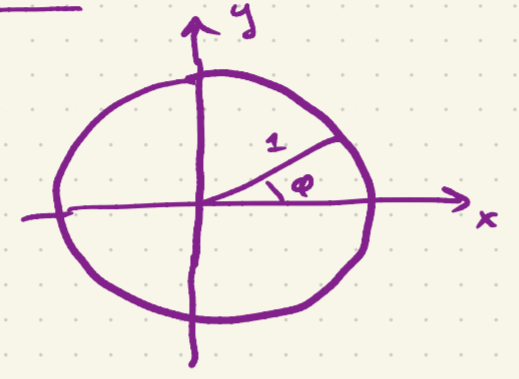
\includegraphics[scale=0.5]{particle_ring}
\end{center}

a) Show that $e^{\pm ikx}$ satisfies the Schr{\"o}dinger equation and $E=\frac{k^2}{2}$

b) Show boundary conditions ... $k\in\mathbf{1}$ i.e. $k=m=0,\pm1,,\pm2,...$

c) Sketch the spectrum for the first 4 energy levels, marking degeneracies

d) Show that, for $m\neq0$, the eigenfunctions can be chosen to be real
and give their forms.

\newpage
\sec{Angular Momentum and Spherical Harmonics}
{\em [Levine pg 101]}
Using $\mathbf{L} = \mathbf{r} \times \mathbf{p}$

a) Show (in Cartesians) $\hat{L}_x = -i(x\frac{d}{dz}-z\frac{d}{dy})$ and find
$\hat{L}_y$ and $\hat{L}_z$

b) Show $[\hat{L}_x,\hat{L}_y]=i\hbar \hat{L}_z$ and find $[\hat{L}_x,\hat{L}_z]$
and $[\hat{L}_y,\hat{L}_z]$

c) Show $[\hat{L}^2,\hat{L}_x] = 0$ and repeat for $[\hat{L}^2,\hat{L}_y]$
and $[\hat{L}^2,\hat{L}_z]$

d) If
\begin{align*}
\mathbf{L}^2 & = -\hbar\mathbf{\Lambda}^2 \\
\mathbf{\Lambda}^2 & = \frac{1}{\text{sin}\theta} \frac{\partial}{\partial\theta}(\text{sin}\theta\frac{\partial}{\partial\theta})
            + \frac{1}{\text{sin}^2\theta}\frac{\partial}{\partial \phi^2}
\end{align*}

show that
\begin{align*}
\hat{L}^2Y^m_n(\Omega) = \hbar^2l(l+1)Y^m_l(\Omega)
\end{align*}

where
\begin{align*}
Y^m_n(\Omega) = \sqrt{\frac{2l+1}{4\pi}\frac{l-|m|!}{l+|m|!}}
            P^{|m|}_e(\text{cos}\theta)e^{im\phi}
\end{align*}

and $P^{|m|}_e(x)$ satisfy differential equations for associated Legender
polynomials

e) Show $\hat{L}_zY^m_n(\Omega) = \hbar m Y^m_n(\Omega)$

f) Defining $\hat{L}_{\pm} = \hat{L}_x \pm i\hat{L}_y$, show
\begin{align*}
\hat{L}_+\hat{L}_- = \hat{L}^2 - \hat{L}^2_z + \hbar\hat{L}_z
\end{align*}

g) Show
\begin{align*}
\hat{L}_{\pm}\ket{l,m} = \sqrt{l(l+1)-m(m\pm1)}\ket{l,m\pm1}
\end{align*}

h) Calculate $\bra{l,m}\hat{L}^2_x\ket{l,m}$ without doing an integral
\newpage
\sec{Coupling Constant Trick}
If $\hat{H}=\hat{T} + \lambda\hat{V}$, $V = \frac{dE(\lambda)}{d\lambda}\bigg|_{\lambda=1}$

a) Check this result for the harmonic oscilator, $\delta$-well, and
even the particle in a box

b) Show that this yields the same result as first-order perturbation
theory

c) If $\hat{H}=\hat{H}_0+\lambda\Delta\hat{V}$, show $E = E_0 + \int^1_0 d\lambda\Delta V(\lambda)$
wher $\Delta V(\lambda) = \bra{\psi_{\lambda}}\Delta\hat{V}\ket{\psi_{\lambda}}$ ({\em Hellmman-Feynman trick})

d) Check c) for harmonic oscillator and $\delta$-well

\newpage
\part{Spin statisics and many-electron atoms}
\newpage
\part{Diatomics and quantum theorems}
\newpage
\part{Electronic stucture theory}
\label{page:end}
\end{document}

\part{Newton for one particle in one dimension: basics}
\newpage
\sec{Harmonic oscillator}

A particle of mass $m$ is subject to a restoring force $-kx$.
\benu
\item What is the potential?
\sol{
\be
F = -kx = -\frac{d V(x)}{d x} \thus V(x) = \frac{1}{2}kx^2
\ee
}
\item What is the equation of motion?
\sol{
\be
F = m\ddot{x} = -kx
\ee
}
\item What is the angular frequency?
\sol{
\be
\omega = \sqrt{\frac{k}{m}}
\ee
}
\item What is the period?
\sol{
\be
\tau = \frac{2\pi}{\omega} = 2\pi\sqrt{\frac{m}{k}}
\ee
}
\item Assuming the particle begins with
velocity $v_0$ at the origin, give its equation of motion.
\sol{
\newline Newton's Second Law for the harmonic oscillator may be written as:
\be
m\ddot{x} = -kx \thus \ddot{x} = -\frac{k}{m}x = -\omega^2 x
\ee
The general solution to this differential equation is a combination of $\sin$ and $\cos$:
\be
x(t) = A\sin{(\omega t)} + B\cos{(\omega t)}
\ee
The particular solution is then found, first using initial position:
\be
x(0) = 0 = A(0) + B(1) = B \thus x(t) = A\sin{(\omega t)}
\ee
Then initial velocity:
\be
v(t) = \frac{d x(t)}{d t} = \omega A \cos{(\omega t)}
\ee
\be
v(0) = v_0 = \omega A (1) \thus A = \frac{v_0}{\omega}
\ee
Therefore:
\be
x(t) = \frac{v_0}{\omega}\sin{(\omega t)} \quad \& \quad v(t) = v_0\cos{(\omega t)}
\ee
}
\item Give formulas for the kinetic and potential energies
as a function of time.
\sol{
\be
T(t) = \frac{1}{2}mv^2 = \frac{m v_0^2}{2}\cos^2{(\omega t)} \quad\quad\quad V(t) = \frac{1}{2}kx^2 = \frac{m v_0^2}{2}\sin^2{(\omega t)}
\ee
}
\item Give a formula for the turning points.  What are the potential and kinetic energies here?
\sol{
\newline At turning points, the position function is at its minimum/maximum. Minimization/maximization of the position function is achieved when $\omega t = \frac{\pi}{2}, \frac{3\pi}{2}, \frac{5\pi}{2}...$ so that the turning point locations, velocity, and times are:
\be
x(t) = \pm \frac{v_0}{\omega} \quad\quad\quad v(t) = 0 \quad\quad\quad t = \frac{\pi}{2\omega}, \frac{3\pi}{2\omega}, \frac{5\pi}{2\omega}...
\ee
The kinetic energy at a turning point is 0 (since the velocity there is 0), while the potential energy is given by:
\be
V = \frac{1}{2}kx^2 = \frac{kv_0^2}{2\omega^2} = \frac{m v_0^2}{2}
\ee
\item Plot $x(t)$, $v(t)$, and both energy components.
\newline All constants were set equal to 1 in the following plots:
\begin{figure*}[h!]
\begin{center}
\begin{subfigure}[h]{.46\textwidth}
    \begin{center}
    \includegraphics[width=0.9\linewidth]{f/1_8_1.png}
    \end{center}
\end{subfigure}
\begin{subfigure}[h]{.46\textwidth}
    \begin{center}
    \includegraphics[width=0.9\linewidth]{f/1_8_2.png}
    \end{center}
\end{subfigure}
\end{center}
\end{figure*}
}
\item If the particle begins instead at $x_0$ with zero
speed, how do all your answers above change?
\sol{
\newline Your answers to 1-4 should remain unchanged. The new equations of motion are:
\be
x(t) = x_0\cos{(\omega t)} \quad \& \quad v(t) = - x_0\omega\sin{(\omega t)}
\ee
The energy expressions:
\be
T(t) = \frac{1}{2}mv^2 = \frac{k x_0^2}{2}\sin^2{(\omega t)} \quad\quad\quad V(t) = \frac{1}{2}kx^2 = \frac{k x_0^2}{2}\cos^2{(\omega t)}
\ee
The turning point expressions:
\be
x(t) = \pm x_0 \quad\quad\quad v(t) = 0 \quad\quad\quad t = \frac{\pi}{\omega}, \frac{2\pi}{\omega}, \frac{3\pi}{\omega}... \quad\quad\quad T(t) = 0 \quad\quad\quad V(t) = \frac{1}{2}kx_0^2
\ee
\newpage
Again, all constants were set equal to 1:
\begin{figure*}[h!]
\begin{center}
\begin{subfigure}[h]{.46\textwidth}
    \begin{center}
    \includegraphics[width=0.9\linewidth]{f/1_9_1.png}
    \end{center}
\end{subfigure}
\begin{subfigure}[h]{.46\textwidth}
    \begin{center}
    \includegraphics[width=0.9\linewidth]{f/1_9_2.png}
    \end{center}
\end{subfigure}
\end{center}
\end{figure*}
}
\enu

%==============================================================================%
\newpage
\sec{Simple functions and complex numbers}
\benu
\item Give a expressions for $\sinh(x)$, $\cosh(x)$, and $\coth(x)$ in terms of
exponentials.
\be
    \sinh{(x)} = \frac{e^x - e^{-x}}{2} \quad\quad \cosh{(x)} = \frac{e^x + e^{-x}}{2} \quad\quad \coth{(x)} = \frac{\cosh{(x)}}{\sinh{(x)}} = \frac{e^x + e^{-x}}{e^x - e^{-x}}
\ee
\item If $x=-\ln(y)/3$, what is $y(x)$?
\be
x(y) = -\frac{\ln{y}}{3} \thus y(x) = e^{-3x}
\ee
\item If $z= (1+i)/(2-i)$, what is $z^3$?  What is $|z|^2$?  What is $z^*$?
\be
z^3 = \frac{(1+i)^3}{(2-i)^3} = \frac{-2+2i}{2-11i} = -\frac{26}{125} - \frac{18}{125}i
\ee
\be
z = \frac{1+i}{2-i} = \frac{1}{5} + \frac{3}{5}i \thus |z| = \sqrt{\frac{10}{25}} = \sqrt{\frac{2}{5}} \thus |z|^2 = \frac{2}{5}
\ee
\be
z^* = \frac{1}{5} - \frac{3}{5}i
\ee
\item What are the cube roots of $i$?  How does your answer change if its $-i$ instead?
\newline Using Euler's formula: $e^{i\theta} = \cos\theta + i\sin\theta$
\be
i = 0 + i(1) = \cos{\left(\frac{\pi}{2} + 2n\pi\right)} + i \sin{\left(\frac{\pi}{2} + 2n\pi\right)} = e^{i\left(\frac{\pi}{2} + 2n\pi\right)}
\ee
\be
z^3 = i \thus z = i^{1/3} = e^{i\left(\frac{\pi}{6} + \frac{2n\pi}{3}\right)} \xrightarrow{n = 0,1,2} z = e^{\frac{\pi}{6}i}, e^{\frac{5\pi}{6}i}, e^{\frac{3\pi}{2}i}
\ee
If we were to use $-i$ instead:
\be
-i = 0 + i(-1) = \cos{\left(-\frac{\pi}{2} + 2n\pi\right)} + i \sin{\left(-\frac{\pi}{2} + 2n\pi\right)} = e^{i\left(-\frac{\pi}{2} + 2n\pi\right)}
\ee
\be
z^3 = -i \thus z = (-i)^{1/3} = e^{i\left(-\frac{\pi}{6} + \frac{2n\pi}{3}\right)} \xrightarrow{n = 1,2,3} z = e^{\frac{\pi}{2}i}, e^{\frac{7\pi}{6}i}, e^{\frac{11\pi}{6}i}
\ee
\item Use Euler's formula, $\exp(i\phi)=cos(\phi)+i\sin(\phi)$ to deduce formulas for $\cos(3\phi)$ and $\sin(5\phi)$ in terms of $\sin(\phi)$ and $\cos(\phi)$.
\newline Beginning with an expression for $e^{3i\phi}$:
\be
\begin{split}
    e^{3i\phi} = e^{i(\phi + \phi + \phi)} &= e^{i\phi}e^{i\phi}e^{i\phi} \\
    &= \left(\cos{\phi} + i\sin{\phi}\right)\left(\cos{\phi} + i\sin{\phi}\right)\left(\cos{\phi} + i\sin{\phi}\right) \\
    &= \cos^3{\phi} - 3\cos{\phi}\sin^2{\phi} + i\left(-\sin^3{\phi} + 3\cos^2{\phi}\sin{\phi}\right)
\end{split}
\ee
We see that:
\be
\begin{split}
    \cos{3\phi} &= \cos^3{\phi} - 3\cos{\phi}\sin^2{\phi} \\
    \sin{3\phi} &= -\sin^3{\phi} + 3\cos^2{\phi}\sin{\phi}
\end{split}
\ee
Now with an expression for $e^{5i\phi}$:
\be
\begin{split}
    e^{5i\phi} = e^{i(\phi + \phi + \phi + \phi + \phi)} &= e^{i\phi}e^{i\phi}e^{i\phi}e^{i\phi}e^{i\phi} \\
    &= \left(\cos{\phi} + i\sin{\phi}\right)^5 \\
    &= \cos^5{\phi} - 10\cos^3{\phi}\sin^2{\phi} + 5\cos{\phi}\sin^4{\phi} \\
    &\hspace{20pt} + i\left(\sin^5{\phi} + 5\cos^4{\phi}\sin{\phi} - 10\cos^2{\phi}\sin^3{\phi}\right)
\end{split}
\ee
We see that:
\be
\begin{split}
    \cos{5\phi} &= \cos^5{\phi} - 10\cos^3{\phi}\sin^2{\phi} + 5\cos{\phi}\sin^4{\phi} \\
    \sin{5\phi} &= \sin^5{\phi} + 5\cos^4{\phi}\sin{\phi} - 10\cos^2{\phi}\sin^3{\phi}
\end{split}
\ee
\enu
%==============================================================================%
\newpage
\sec{Differentiation}
\benu
\item What is derivative of $x^p$?  $\sin(x)$? $\cos(x)$?  $\coth(x)$?  $\sin^{-1}(x)$?
\be
\frac{d}{dx} \left(x^p\right) = px^{p-1} \quad \frac{d}{dx} \left(\sin{(x)}\right) = \cos{(x)} \quad \frac{d}{dx} \left(\cos{(x)}\right) = -\sin{(x)}
\ee
\be
\frac{d}{dx} \left(\coth{(x)}\right) = -\text{csch}^2(x) \quad\quad \frac{d}{dx} \left(\sin^{-1}{(x)}\right) = \frac{1}{\sqrt{1-x^2}}
\ee
\item What function is proportional to its own derivative?
\newline Both $a$ and $b$ are constants:
\be
f(x) = a e^{b x} \hspace{2pt} \rightarrow \hspace{2pt} \frac{d f(x)}{dx} = b \left(a e^{b x}\right) \propto f(x)
\ee
\item What is derivative of $\ln(\ln(x))$?
\newline Use the chain rule:
\be
\frac{d}{dx} \left(\ln{(\ln{(x)})}\right) = \left(\frac{1}{\ln{(x)}}\right)\left(\frac{1}{x}\right) = \frac{1}{x\ln{(x)}}
\ee
\item If $f(u)=u^{1/3}$, and $u(y)=-sin(y)$, and $y(x)=1/\sqrt{1-x^2}$, what is 
$df/dx$?
\be
\frac{df}{dx} = \frac{df}{du} \frac{du}{dy} \frac{dy}{dx} = \left[\frac{1}{3}u^{-2/3}\right]\left[-\cos{y}\right]\left[\frac{x}{(1-x^2)^{\frac{3}{2}}}\right] = -\frac{x\cos{\left(\frac{1}{\sqrt{1-x^2}}\right)}}{3(1-x^2)^{\frac{3}{2}}\left(-\sin{\left(\frac{1}{\sqrt{1-x^2}}\right)}\right)^{2/3}}
\ee
\item What is the position and value of any extrema of $f(x)=2x^2-x^4$?  Which are
maxima and which are minima?
\be
f(x) = 2x^2 - x^4 \thus \frac{df}{dx} = 4x - 4x^3 = 4x(1 - x^2) = 4x(1 - x)(1 + x) = 0
\ee
Therefore, there are three extrema, at $x = -1, 0, \text{ and } 1$. We see that:
\be
f(-1) = 1 \quad\quad\quad f(0) = 0 \quad\quad\quad f(1) = 1
\ee
Signifying that $x = 0$ is a minimum and $x = \pm 1$ are maxima.
\enu
%==============================================================================%
\newpage
\sec{Integration}
\benu
\item Find the integrals of $\sinh(x)$, $\cosh(x)$, and $\coth(x)$.
\be
\int\sinh{(x)} \hspace{2pt} dx = \cosh{(x)} \quad \int\cosh{(x)} \hspace{2pt} dx = \sinh{(x)} \quad \int\coth{(x)} \hspace{2pt} dx = \ln{\left(\sinh{(x)}\right)}
\ee
\item Integrate $\sin^{-1}(x)$.
\newline Integrate this by parts: $\int u dv = uv - \int v du$
\be
\begin{split}
    u &= \sin^{-1}{(x)} \\
    dv &= dx
\end{split}
\quad\quad\quad
\begin{split}
    du &= \frac{dx}{\sqrt{1-x^2}} \\
    v &= x
\end{split}
\ee
\be
\int \sin^{-1}{(x)}dx = x\sin^{-1}{(x)} + \int \frac{x}{\sqrt{1-x^2}} \hspace{2pt} dx = x\sin^{-1}{(x)} + \sqrt{1-x^2}
\ee
\item Find the area between 0 and 2 under the curve $\exp(-x) x$.
\newline Again, integrate this by parts:
\be
\begin{split}
    u &= x \\
    dv &= e^{-x} \hspace{2pt} dx
\end{split}
\quad\quad\quad
\begin{split}
    du &= dx \\
    v &= -e^{-x}
\end{split}
\ee
\be
\int_0^2 x e^{-x} \hspace{2pt} dx = -xe^{-x} - e^{-x} \bigg|_0^2 = 1 - 3e^{-2}
\ee
\item Find $\int_0^{\infty} dx\, exp(-x^2/2)$.
\newline Using the Gaussian integral formula: $\int_{-\infty}^\infty e^{-ax^2} dx = \sqrt{\frac{\pi}{a}}$
\be
\int_0^\infty e^{-\frac{x^2}{2}} \hspace{2pt} dx = \frac{1}{2} \int_{-\infty}^\infty e^{-\frac{x^2}{2}} \hspace{2pt} dx = \frac{1}{2} \sqrt{2\pi} = \sqrt{\frac{\pi}{2}}
\ee
\item Find $\int_0^{\infty} dx\, x^6\, exp(-x^2/2)$.
\newline Using the integral formula: $\int_0^\infty x^{2n} e^{-ax^2} dx = \frac{(2n-1)!!}{a^n 2^{n+1}}\sqrt{\frac{\pi}{a}}$
\be
\int_0^\infty x^6 e^{-\frac{x^2}{2}} \hspace{2pt} dx = \frac{(5)!!}{(\frac{1}{2})^3 \times 2^4} \sqrt{2\pi} = \frac{15}{2}\sqrt{2\pi} = 15 \sqrt{\frac{\pi}{2}}
\ee
\enu
%==============================================================================%
\newpage
\sec{Differential equations}
\benu
\item If $y'=-\alpha y$ and $y(0)=1$, what is $y(2)$?
\be
\frac{dy}{dx} = -\alpha y \thus \frac{dy}{y} = -\alpha dx \thus \ln{y} = -\alpha x + C \thus y(x) = Ae^{-\alpha x} \\
\ee
\be
y(0) = 1 = A \thus y(x) = e^{-\alpha x}
\ee
Therefore we have determined that:
\be
y(2) = e^{-2\alpha}
\ee
\item If $y'=-\alpha y^2$ and $y(0)=1$, what is $y(2)$?
\be
\frac{dy}{dx} = -\alpha y^2 \thus \frac{dy}{y^2} = -\alpha dx \thus -\frac{1}{y} = -\alpha x + C \thus y(x) = \frac{1}{\alpha x - C} \\
\ee
\be
y(0) = 1 = \frac{1}{-C} \thus C = -1 \thus y(x) = \frac{1}{\alpha x + 1}
\ee
Therefore we have determined that:
\be
y(2) = \frac{1}{2\alpha + 1}
\ee
\item If $y'=\alpha\sin(x)$ and $y(0)=1$, what is $y(2)$?
\be
\frac{dy}{dx} = \alpha \sin{(x)} \thus dy = \alpha \sin{(x)} dx \thus y(x) = -\alpha \cos{(x)} + C 
\ee
\be
y(0) = 1 = -\alpha + C \thus C = 1 + \alpha \thus y(x) = \alpha (1 - \cos{(x)}) + 1
\ee
Therefore we have determined that:
\be
y(2) = \alpha (1 - \cos{(2)}) + 1
\ee
\item If $y''=F$, what is the general solution and how many free constants must it have?
\newline There are two free constants in the general solution (due to the double integration), denoted here by $A$ and $B$:
\be
y'' = F \thus y'(x) = Fx + A \thus y(x) = \frac{F}{2}x^2 + Ax + B
\ee
\item In previous question, if $F=1$, and $y(0)=1$ and $y'(0)=0$, what is $y(2)$?
\be
y'(0) = 0 = A \quad\quad\quad y(0) = 1 = B \quad\quad \thus \quad\quad y(x) = \frac{1}{2}x^2 + 1 \thus y(2) = 3
\ee
\item In previous question, if $F=1$, and $y'(0)=1$ and $y(0)=0$, what is $y(2)$?
\be
y'(0) = 1 = A \quad\quad\quad y(0) = 0 = B \quad\quad \thus \quad\quad y(x) = \frac{1}{2}x^2 + x \thus y(2) = 4
\ee
\enu
%==============================================================================%
\newpage
\sec{Taylor series}
\benu
\item Give the general formula for the coefficient of $x^n$ when $f(x)$ is expanded about $x=0$.
\be
f(x) = \sum_{n=0}^\infty \frac{f^{(n)}(0)}{n!}x^n \thus \text{the coefficient of } x^n \text{ is: } \frac{f^{(n)}(0)}{n!}
\ee
\item Give Taylor series for $e^x$, $e^{-x}$, $\cos(x)$, $\sin(x)$, $\tanh(x)$. In each case, give the first three non-zero terms, and a formula for the $k$-th term.
\newline In the following series, $B_n$ represents the $n$th Bernoulli number:
\be
\begin{split}
    e^x &= \sum_{k=0}^\infty \frac{x^k}{k!} \\
    &= 1 + x + \frac{x^2}{2} + ... \\
\end{split}
\quad\quad
\begin{split}
    e^{-x} &= \sum_{k=0}^\infty \frac{(-x)^k}{k!} \\
    &= 1 - x + \frac{x^2}{2} + ... \\
\end{split}
\quad\quad
\begin{split}
    \cos{(x)} &= \sum_{k=0}^\infty \frac{(-1)^k}{(2k)!}x^{2k} \\
    &= 1 - \frac{x^2}{2} + \frac{x^4}{24} + ... \\
\end{split}
\ee
\be
\begin{split}
    \sin{(x)} &= \sum_{k=0}^\infty \frac{(-1)^k}{(2k + 1)!}x^{2k + 1} \\
    &= x - \frac{x^3}{6} + \frac{x^5}{120} + ... \\
\end{split}
\quad\quad\quad
\begin{split}
    \tanh{(x)} &= \sum_{k=1}^\infty \frac{B_{2k}4^k(4^k - 1)}{(2k)!}x^{2k - 1} \\
    &= x - \frac{x^3}{3} + \frac{2x^5}{15} + ... \\
\end{split}
\ee
\item Compare $\sin x$ with its third order expansion by plotting it for $x=0$ to $2$.
\begin{center}
\includegraphics[width=0.7\linewidth]{f/6_3_1.png}
\end{center}
\item Repeat previous question for $(1+x)^{p}$ and $\ln(1+x)$.
\newline The Taylor series for $(1+x)^p$ is:
\be
(1+x)^p \approx 1 + px + \frac{p(p-1)}{2}x^2 + \frac{p(p-1)(p-2)}{6}x^3 + ...
\ee
Plotting this for $p = 4$ and $p = 7$:
\begin{figure*}[h!]
\begin{center}
\begin{subfigure}[h]{.46\textwidth}
    \begin{center}
    \includegraphics[width=0.9\linewidth]{f/6_4_1.png}
    \end{center}
\end{subfigure}
\begin{subfigure}[h]{.48\textwidth}
    \begin{center}
    \includegraphics[width=0.9\linewidth]{f/6_4_2.png}
    \end{center}
\end{subfigure}
\end{center}
\end{figure*}
Now for $\ln{(x)}$:
\begin{center}
\includegraphics[width=0.7\linewidth]{f/6_4_3.png}
\end{center}
\item Repeat previous question for $\ln((1+x)/(1-x))$ and $((1+x)/(1-x))^p$.
\newline The Taylor series for $\frac{(1+x)^p}{(1-x)^p}$ is:
\be
\frac{(1+x)^p}{(1-x)^p} \approx 1 + 2px + 2p^2x^2 + \frac{2}{3}\left(p+2p^3\right)x^3 + ...
\ee
Plotting this for $p = 4$ and $p = 7$:
\begin{figure*}[h!]
\begin{center}
\begin{subfigure}[h]{.46\textwidth}
    \begin{center}
    \includegraphics[width=0.9\linewidth]{f/6_5_1.png}
    \end{center}
\end{subfigure}
\begin{subfigure}[h]{.48\textwidth}
    \begin{center}
    \includegraphics[width=0.9\linewidth]{f/6_5_2.png}
    \end{center}
\end{subfigure}
\end{center}
\end{figure*}
Now for $\ln{(\frac{1+x}{1-x})}$:
\begin{center}
\includegraphics[width=0.7\linewidth]{f/6_5_3.png}
\end{center}
\item For previous two questions, give explicit formulas for special cases $p=-1,1/2,$ and $-1/2$.
\newline For $p = -1$:
\be
(1 + x)^{-1} = \frac{1}{1 + x} = \sum_{k=0}^\infty (-x)^k \\
\ee
\begin{center}
    \&
\end{center}
\be
\left(\frac{1+x}{1-x}\right)^{-1} = (1-x)\left(\frac{1}{1 + x}\right) = (1-x) \sum_{k=0}^\infty (-x)^k
\ee
For $p = \frac{1}{2}$:
\be
\begin{split}
(1 + x)^{\frac{1}{2}} = \sqrt{1 + x} = \sum_{k=0}^\infty \begin{pmatrix} 1/2 \\  k \end{pmatrix} x^k \\
\end{split}
\ee
\begin{center}
    \&
\end{center}
\be
\left(\frac{1+x}{1-x}\right)^{\frac{1}{2}} = \left(\sqrt{1 + x}\right)\left(\frac{1}{\sqrt{1 - x}}\right) = \left[\sum_{k=0}^\infty \begin{pmatrix} 1/2 \\  k \end{pmatrix} x^k\right]\left[\sum_{k=0}^\infty \begin{pmatrix} -1/2 \\  k \end{pmatrix} (-x)^k\right]
\ee
For $p = -\frac{1}{2}$:
\be
(1 + x)^{-\frac{1}{2}} = \frac{1}{\sqrt{1 + x}} = \sum_{k=0}^\infty \begin{pmatrix} -1/2 \\  k \end{pmatrix} x^k \\
\ee
\begin{center}
    \&
\end{center}
\be
\left(\frac{1+x}{1-x}\right)^{-\frac{1}{2}} = \left(\sqrt{1 - x}\right)\left(\frac{1}{\sqrt{1 + x}}\right) = \left[\sum_{k=0}^\infty \begin{pmatrix} 1/2 \\  k \end{pmatrix} (-x)^k\right]\left[\sum_{k=0}^\infty \begin{pmatrix} -1/2 \\  k \end{pmatrix} x^k\right]
\ee
Where we have used a binomial series notation above. There is a great explanation of this notation on Wikipedia's 'Taylor series' page.
\item Solve $\tan x = (1 +c) x$ for $0 < c << 1$ as a power series in $c$.  Find the first three non-zero terms.  Check your answer for $c=0.2$.
\be
\frac{\tan{(x)}}{x} = \left(\frac{1}{x}\right)\left(x + \frac{x^3}{3} + \frac{2x^5}{15}\right) = 1 + \frac{x^2}{3} + \frac{2x^4}{15} = 1 + c
\ee
Solving this expression for $x$:
\be
x = \frac{1}{2}\sqrt{-5 + \sqrt{25 + 120c}} \quad \xrightarrow{c = 0.2} \quad x = 0.707107
\ee
Checking this: 
\be
\tan{\left(0.707107\right)} = (1 + 0.2) \times 0.707107 \thus 0.85451 = 0.848528
\ee
\enu
\newpage
%==============================================================================%
\newpage
\sec{Newton's 2nd law}
\benu
\item State Newton's second law for a particle in a potential $V(x)$ with mass $m$.
\be
F = m \ddot{x} = -\frac{d V(x)}{d x}
\ee
\item Show that the change in momentum over an interval of time is the time-integral of the force.
\be
F  = m\dot{v} = \dot{p} = \frac{d p}{d t} \thus F dt = dp \thus \int F dt = \int dp = \Delta p
\ee
\item By multiplying each side by $\dot x$ and integrating, prove energy is conserved.
\newline By multiplying by $\dot{x}$ on both sides, the following simplification is made to Newton's Second Law:
\be
m \ddot{x} = -\frac{d V(x)}{d x} \thus m \ddot{x} \dot{x} = -\frac{d V(x)}{d x} \frac{d x}{d t} = -\frac{d V(x)}{d t}
\ee
Using this, we can prove that the energy remains constant over time:
\be
E = \frac{1}{2} m \dot{x}^2 + V(x) \thus \frac{d E}{d t} = m \ddot{x} \dot{x} + \frac{d V(x)}{d t} = 0
\ee
\item How many free constants should there be in the general solution?
\newline There should be 2 free constants: initial velocity and initial position ($v_0$ and $x_0$).
\item What information is given in an initial value problem?
\newline The 2 free constants in the general solution are given, allowing us to determine a particular solution.
\enu
%==============================================================================%
\newpage
\sec{Atomic units}
Give all answers in SI units.
These are then the atomic units of each quantity.  If you use atomic units
in your calculations, results appear in these units.
\benu
\item What angular frequency (in SI units) corresponds to 1 Hartree of energy?
\newline Noting that $1$ Hartree = $4.359745 \times 10^{-18} \text{ J}$:
\be
\omega = \frac{E}{\hbar} = \frac{4.359745 \times 10^{-18} \text{ J}}{1.0545718 \times 10^{-34} \text{ J} \cdot \text{s}} = 4.1341377 \times 10^{16} \text{ s}^{-1}
\ee
\item What period is this?  In fact, the atomic unit of time is just $1/\omega$, so figure this value out.
\be
\tau = \frac{1}{\omega} = \frac{1}{4.1341377 \times 10^{16} \text{ s}^{-1}} = 2.41888413 \times 10^{-17} \text{ s}
\ee
\item What force constant would it imply for a single electron? Interestingly, a rubber band is typical 1-5 N/m.
\newline Noting that $\omega = \sqrt{\frac{k}{m_e}}$:
\be
\begin{split}
    k = m_e \omega^2 = \left(9.109383 \times 10^{-31} \text{ kg}\right)\left(4.1341377 \times 10^{16} \text{ s}^{-1}\right)^2 &= 1556.8932334 \text{ kg/s}^2 \\
    &= 1556.8932334 \text{ N/m}
\end{split}
\ee
\item What velocity does a free electron have with this energy? What fraction of the speed of light is this?
\be
v = a_0 \omega = \left(0.529177 \times 10^{-10} \text{ m}\right)\left(4.1341377 \times 10^{16} \text{ s}^{-1}\right) = 2.18769156 \times 10^{6} \text{m/s}
\ee
\be
\frac{v}{c} = \frac{2.18769156 \times 10^{6} \text{ m/s}}{2.99792458 \times 10^{8} \text{ m/s}} = 0.00729735355
\ee
\item What is the atomic amount of momentum?
\be
p = \frac{\hbar}{a_0} = \frac{1.0545718 \times 10^{-34} \text{ J} \cdot \text{s}}{0.529177 \times 10^{-10} \text{ m}} = 1.9928519 \times 10^{-24} \text{ kg}\cdot\text{m/s}
\ee
\enu
%==============================================================================%
\newpage
\sec{Free particle}
\benu
\item For a free particle of mass $m$, give the general solution to Newton's equation.
\be
F = m\ddot{x} = 0 \thus x(t) = A t + B \thus x(t) = v_0 t + x_0
\ee
\item Give the solution that has initial velocity $v_0$ and starts at the origin.
\be
x(t) = v_0 t
\ee
\item How long will it take such a particle to travel a distance $a$?
\be
x(t) = a = v_0 t \thus t = \frac{a}{v_0}
\ee
\item Is the energy conserved here and, if so, what is its value?
\newline Yes, energy is conserved. It's value is equal to the kinetic energy of the free particle:
\be
E = T + V = T = \frac{1}{2}mv_0^2
\ee
\item Plot $x$ as a function of time.  Repeat, starting from both positive and negative values
of $x_0$.  Describe the shape of the curves.
\newline In the following plot, $v_0$ was set to 1. The position function is linear with time for a free particle.
\begin{center}
\includegraphics[width=0.7\linewidth]{f/9_5_1.png}
\end{center}
\newpage
\item Plot $v$ as a function of time and describe the curve.
\newline In the following plot, $v_0$ was set to 1. The velocity remains constant for a free particle.
\begin{center}
\includegraphics[width=0.68\linewidth]{f/9_6_1.png}
\end{center}
\enu
%==============================================================================%
\newpage
\sec{Constant force}
\benu
\item Given the general solution to the equations of motion in a constant opposing force $-F_0$, $F_0>0$.
\be
    F = m\ddot{x} = -F_0 \thus \ddot{x}(t) = -\frac{F_0}{m} \thus \dot{x}(t) = - \frac{F_0}{m} t + v_0 \thus x(t) = - \frac{F_0}{2m} t^2 + v_0 t + x_0
\ee
\item What is the potential for such a force?
\be
- \frac{d V(x)}{dx} = - F_0 \quad \longrightarrow \quad V(x) = F_0 x
\ee
\item What condition guarantees the particle returns to its starting point?  For the next few questions, assume that condition is fulfilled.
\newline In order for the particle to return to its starting point, $v_0 > 0$.
\item Derive formulas for both the position, $x_{tp}$, and time, $t_{tp}$, at which the particle turns around.
\newline At the turning point, $\dot{x}(t) = 0$:
\be
\dot{x}(t_{tp}) = 0 = - \frac{F_0}{m} t_{tp} + v_0 \thus t_{tp} = \frac{m v_0}{F_0}
\ee
The turning point location is therefore:
\be
x_{tp} = x(t_{tp}) = -\frac{F_0}{2m} t_{tp}^2 + v_0 t_{tp} + x_0 = \frac{m v_0^2}{2F_0} +  x_0
\ee
\item Derive a formula for the return time, $t_r$, at which it comes back to the starting point. How is it related to $t_{tp}$?
\newline The return time is found to be double that of the turning point time:
\be
x(t_r) = x_0 = - \frac{F_0}{2m} t_r^2 + v_0 t_r + x_0 \thus \left(\frac{F_0}{2m} t_r - v_0\right)t_r = 0 \thus t_r = \frac{2mv_0}{F_0}
\ee
\item Derive a formula for $v_r$, the velocity at the return time.
\be
v_r = \dot{x}(t_r) = - \frac{F_0}{m} t_r + v_0 = - v_0 
\ee
\item Plot $x(t)$, $v(t)$, and the kinetic, potential, and total energies.
\newline All constants were set equal to 1 in the following plots:
\begin{figure*}[h!]
\begin{center}
\begin{subfigure}[h]{.46\textwidth}
    \begin{center}
    \includegraphics[width=0.9\linewidth]{f/10_7_1.png}
    \end{center}
\end{subfigure}
\begin{subfigure}[h]{.46\textwidth}
    \begin{center}
    \includegraphics[width=0.9\linewidth]{f/10_7_2.png}
    \end{center}
\end{subfigure}
\end{center}
\end{figure*}
\item If I double $F_0$, keeping $v_0$ fixed, what happens to $x_{tp}$, $t_r$, and $v_r$?
\newline If you double $F_0$: $x_{tp}$ and $t_{r}$ are halved, while $v_{r}$ remains the same.
\item Plot $t_r$ as a function of $v_0$, for both positive and negative values.
\newline $t_r$ is linear with $v_0$:
\begin{center}
\includegraphics[width=0.7\linewidth]{f/10_9_1.png}
\end{center}
\enu
%==============================================================================%
\newpage
\sec{Time-dependent forces}
For $F(t)=-Gt$, $G >0$, and initially $v=v_0$, but $x=0$.
\benu
\item Solve Newton's equation for $x(t)$.
\be
F(t) = m \ddot{x} =  - Gt  \thus \ddot{x} = - \frac{G}{m}t \thus \dot{x}(t) = - \frac{G}{2m}t^2 + v_0 \thus x(t) = - \frac{G}{6m}t^3 + v_0 t
\ee
\item Give formulas for the turning point and time, and the time
and velocity when it returns to its initial position.
\newline At the turning point, the velocity is 0. We can use this to determine the time it takes to reach the turning point:
\be
\dot{x}(t) = 0 = - \frac{G}{2m}t_{tp}^2 + v_0 \thus t_{tp}^2 = \frac{2mv_0}{G} \thus t_{tp} = \sqrt{\frac{2mv_0}{G}}
\ee
The position of the turning point is determined to be:
\be
\begin{split}
    x_{tp} = x(t_{tp}) &= - \frac{G}{6m}\left(\sqrt{\frac{2mv_0}{G}}\right)^3 + v_0 \left(\sqrt{\frac{2mv_0}{G}}\right) \\
    &= - \frac{G}{6m}\left(\frac{2mv_0}{G}\right)\left(\sqrt{\frac{2mv_0}{G}}\right) + v_0 \left(\sqrt{\frac{2mv_0}{G}}\right) \\
    &= - \frac{v_0}{3}\left(\sqrt{\frac{2mv_0}{G}}\right) + v_0 \left(\sqrt{\frac{2mv_0}{G}}\right) \\
    &= \frac{2v_0}{3}\left(\sqrt{\frac{2mv_0}{G}}\right) \\
\end{split}
\ee
The time it takes to return to the initial position may be found in the following manner:
\be
x(t_r) = 0 = -\frac{G}{6m}t_r^3 + v_0 t_r \thus \left(-\frac{G}{6m}t^2 + v_0\right)t \thus t_r^2 = \frac{6mv_0}{G} \thus t_r = \sqrt{\frac{6mv_0}{G}}
\ee
The velocity at this initial position is therefore:
\be
v_r = \dot{x}(t_r) = - \frac{G}{2m}t_r^2 + v_0 = - \frac{G}{2m}\left(\frac{6mv_0}{G}\right) + v_0 = -3v_0 + v_0 = -2v_0
\ee
\item How do all above quantities change if $G$ is halved, keeping $v_0$ fixed?
\newline If $G$ were cut in half: $x_{tp}, t_{tp},$ and $ t_r$ would all increase by a factor of $\sqrt{2}$, while $v_r$ would remain unchanged.
\item How do they all change if $v_0$ is doubled, keeping $G$ fixed?
\newline If $v_0$ is doubled: $x_{tp}, t_{tp},$ and $ t_r$ would all increase by a factor of $\sqrt{2}$, while $v_r$ would double.
\item Plot $x$ and $v$ as functions of $t$.
\newline All constants were set equal to 1 in the following plot:
\begin{center}
\includegraphics[width=0.7\linewidth]{f/11_5_1.png}
\end{center}
\enu
%==============================================================================%
\newpage
\sec{Velocity-dependent forces}
\benu
\item If $F$ depends only on $v$, write a general solution to Newton's equation.
\be
    F = m\ddot{x} = -\alpha v \thus \ddot{x} = \dot{v} = -\frac{\alpha}{m} v \thus v(t) = Ae^{-\frac{\alpha}{m} t}
\ee
\item Find the trajectory of a particle of mass $m$ in a potential $F=-\alpha v$.
\be
\begin{split}
    F = m\ddot{x} = -\alpha v \thus \ddot{x} = \dot{v} = -\frac{\alpha}{m} v \thus \frac{dv}{v} &= -\frac{\alpha}{m} dt \\
    \ln{v} &= -\frac{\alpha}{m}t + C \\
    v(t) &= Ae^{-\frac{\alpha}{m} t} \thus v(t) = v_0e^{-\frac{\alpha}{m} t}
\end{split}
\ee
\be
\begin{split}
    \dot{x}(t) = v_0e^{-\frac{\alpha}{m} t} \thus x(t) = -\frac{mv_0}{\alpha}e^{-\frac{\alpha}{m} t} + C \thus x(t) &= -\frac{mv_0}{\alpha}e^{-\frac{\alpha}{m} t} + \frac{mv_0}{\alpha} + x_0 \\
    x(t) &= \frac{mv_0}{\alpha}\left(1 - e^{-\frac{\alpha}{m} t}\right) + x_0
\end{split}
\ee
\item If the particle begins at the origin with velocity $v_0$, derive formulas for
how long it takes to halve its speed, and where it is when that happens.
\newline To determine the time in which the particle halves its speed:
\be
\frac{v_0}{2} = v_0e^{-\frac{\alpha}{m} t_{1/2}} \thus t_{1/2} = \frac{m}{\alpha}\ln{2}
\ee
At this time, the particle is located at:
\be
x(t) = \frac{mv_0}{\alpha}\left(1 - e^{-\frac{\alpha}{m} t}\right) \thus x\left(t_{1/2}\right) = \frac{mv_0}{2\alpha}
\ee
\item Plot $x, v$ and kinetic energy as a function of time.
\begin{figure*}[h!]
\begin{center}
\begin{subfigure}[h]{.46\textwidth}
    \begin{center}
    \includegraphics[width=0.9\linewidth]{f/12_4_1.png}
    \end{center}
\end{subfigure}
\begin{subfigure}[h]{.48\textwidth}
    \begin{center}
    \includegraphics[width=0.9\linewidth]{f/12_4_2.png}
    \end{center}
\end{subfigure}
\end{center}
\end{figure*}
\enu
%==============================================================================%
\newpage
\sec{Damped harmonic oscillator}
\benu
\item If a harmonic oscillator of mass $m$ has force constant $k$ and frictional force $-m\gamma v$, 
write its equation of motion.
\be
F = m\ddot{x} = -m \gamma v - kx
\ee
\item Write a solution in terms of exponentials, and find the formula the complex frequencies must
satisfy.
\be
m\ddot{x} = -m \gamma \dot{x} - kx \thus \ddot{x} = - \gamma \dot{x} - \omega^2 x \thus \ddot{x} + \gamma \dot{x} + \omega^2 x = 0
\ee
Using $x(t) = Ce^{zt}$ as a guess:
\be
\ddot{x} + \gamma \dot{x} + \omega^2 x = 0 \thus \left(z^2 + \gamma z + \omega^2\right)x(t) = 0
\ee
\be
z = \frac{-\gamma \pm \sqrt{\gamma^2 - 4\omega^2}}{2} = -\frac{\gamma}{2} \pm \frac{1}{2}\sqrt{\gamma^2 - 4\omega^2}
\ee
\item Show the explicit form of the general solution for an underdamped case.
\newline In the underdamped case, $\gamma^2 < 4\omega^2$, signifying that $z$ is complex. We see that:
\be
z = -\frac{\gamma}{2} \pm \frac{1}{2}\sqrt{\gamma^2 - 4\omega^2} = -\frac{\gamma}{2} \pm \frac{1}{2}i\sqrt{4\omega^2 - \gamma^2} = -\frac{\gamma}{2} \pm i \Tilde{\omega}
\ee
Where $\Tilde{\omega} = \frac{1}{2}\sqrt{4\omega^2 - \gamma^2}$. The general solution is therefore:
\be
x(t) = e^{-\frac{\gamma}{2}t} \left[Ce^{i\Tilde{\omega}t} + De^{-i\Tilde{\omega}t}\right] = e^{-\frac{\gamma}{2}t} \left[A\cos{\Tilde{\omega}t} + B\sin{\Tilde{\omega}t}\right] 
\ee
\item Repeat for the overdamped case.
\newline In the overdamped case, $\gamma^2 > 4\omega^2$, signifying that $z$ is real. We see that:
\be
z = -\frac{\gamma}{2} \pm \frac{1}{2}\sqrt{\gamma^2 - 4\omega^2} = -\frac{\gamma}{2} \pm \Omega
\ee
Where $\Omega = \frac{1}{2}\sqrt{\gamma^2 - 4\omega^2}$. The general solution is therefore:
\be
x(t) = e^{-\frac{\gamma}{2}t} \left[Ce^{\Omega t} + De^{-\Omega t}\right] = e^{-\frac{\gamma}{2}t} \left[A\cosh{\Omega t} + B\sinh{\Omega t}\right] 
\ee
\item Repeat for the critically damped case.
\newline In the critically damped case, $\gamma^2 = 4\omega^2$. We see that $z = -\frac{\gamma}{2}$, yielding a general solution of:
\be
x(t) = e^{-\frac{\gamma}{2}t} \left[A + Bt\right]
\ee
\enu
%==============================================================================%
\newpage
\sec{Reflection}
A hard wall is positioned at $x=l$, and a particle is moving toward it at the
origin with velocity $v_0$ and mass $m$.
\benu
\item Derive an expression for the time when the particle hits the wall.
\newline The particle must move a distance $l$ at a constant speed of $v_0$:
\be
t = \frac{l}{v_0}
\ee
\item How long before the particle is back where it started? Compare this time
to the previous answer and explain why.
\newline The particle must move a distance $2l$ at a constant speed of $v_0$:
\be
t = \frac{2l}{v_0}
\ee
This time is exactly double that of the first answer, signifying that the reflection at the hard wall is instant.
\item Plot $x$ and $v$ and the kinetic, potential, and total energies as a function of time.
\newline All constants are set equal to 1 in the following plots. Note that all energies are constant: kinetic energy is set at $\frac{1}{2}mv_0^2$, potential energy is an arbitrary constant (we can assume 0), and the total energy is just the sum of these two constants:
\begin{figure*}[h!]
\begin{center}
\begin{subfigure}[h]{.30\textwidth}
    \begin{center}
    \includegraphics[width=0.9\linewidth]{f/14_3_1.png}
    \end{center}
\end{subfigure}
\begin{subfigure}[h]{.30\textwidth}
    \begin{center}
    \includegraphics[width=0.9\linewidth]{f/14_3_2.png}
    \end{center}
\end{subfigure}
\begin{subfigure}[h]{.32\textwidth}
    \begin{center}
    \includegraphics[width=0.9\linewidth]{f/14_3_3.png}
    \end{center}
\end{subfigure}
\end{center}
\end{figure*}
\item Next assume that the wall is soft, i.e., $V(x) = k(x-l)^2/2 $ for $x>l$,
and
repeat all the previous questions.
\newline We need to find the time it takes for the particle to turn around after crossing the $x=l$ boundary. For $x>l$:
\be
F = m\ddot{x} = -\frac{dV}{dx} = k(l-x) \thus \ddot{x} = \frac{k}{m}(l-x) = \omega^2 (l-x)
\ee
This equation has the following solution (if we say $x(0) = l$ and $v(0) = v_0$):
\be
x(t) = l + A\cos{(\omega t)} + B\sin{(\omega t)} \thus x(t) = l + \frac{v_0}{\omega}\sin{(\omega t)}
\ee
At the turning point, we see that:
\be
\dot{x}(t) = 0 = v_0\cos{(\omega t)} \thus t = \frac{\pi}{2\omega} = \frac{\pi}{2}\sqrt{\frac{m}{k}}
\ee
Therefore, the total turnaround time (starting from the origin) is $t = \frac{l}{v_0} + \frac{\pi}{2}\sqrt{\frac{m}{k}}$. The time it takes to return to the origin is $t = \frac{2l}{v_0} + \pi\sqrt{\frac{m}{k}}$.
\begin{figure*}[h!]
\begin{center}
\begin{subfigure}[h]{.30\textwidth}
    \begin{center}
    \includegraphics[width=0.9\linewidth]{f/14_4_1.png}
    \end{center}
\end{subfigure}
\begin{subfigure}[h]{.30\textwidth}
    \begin{center}
    \includegraphics[width=0.9\linewidth]{f/14_4_2.png}
    \end{center}
\end{subfigure}
\begin{subfigure}[h]{.32\textwidth}
    \begin{center}
    \includegraphics[width=0.9\linewidth]{f/14_4_3.png}
    \end{center}
\end{subfigure}
\end{center}
\end{figure*}
\item What happens to all your answers as $k\to\infty$?
\newline As $k \rightarrow \infty$, the potential becomes more like a hard wall at $x=l$; all of the soft wall answers become equal to the hard wall answers.
\enu
%==============================================================================%
\newpage 
\sec{Infinite linear well}
A particle of mass $m$ is in a potential well $V(x)=F_0 |x|$.
\benu
\item What is the force as a function of $x$?
\be
F = -\frac{d V(x)}{dx} = -F_0 \hspace{2pt} \text{sgn}(x)
\ee
\item What is the equation of motion?
\be
F = m\ddot{x} = -F_0 \hspace{2pt} \text{sgn}(x) \thus m\ddot{x} = -F_0 \text{ (for positive x} )
\ee
\item What is the period?
\newline Determine the time at which the position function returns to 0:
\be
\begin{split}
    x(t) = -\frac{F_0}{2m}t^2 + v_0t \thus 0 &= -\frac{F_0}{2m}t^2 + v_0t \\
    0 &= t\left(-\frac{F_0}{2m}t + v_0\right) \thus t = \frac{2mv_0}{F_0} \thus \tau = \frac{4mv_0}{F_0}
\end{split}
\ee
\item Assuming the particle begins with velocity $v_0$ at the origin, find $x(t)$.
\be
    m\ddot{x} = -F_0 \thus \ddot{x}(t) = -\frac{F_0}{m} \thus \dot{x}(t) = -\frac{F_0}{m}t + v_0 \thus x(t) = -\frac{F_0}{2m}t^2 + v_0t
\ee
\item Give formulas for the kinetic and potential energies as a function of time.
\be
T(t) = \frac{1}{2}m\dot{x}^2 = \frac{m}{2}\left(-\frac{F_0}{m}t + v_0\right)^2 \quad\quad\quad V(t) = F_0 |x(t)| = F_0 \left|-\frac{F_0}{2m}t^2 + v_0t\right|
\ee
\item Give a formula for the turning points.  What are the potential and kinetic energies here?
\newline At the turning points, $\dot{x}(t) = 0$:
\be
\dot{x}(t) = 0 = -\frac{F_0}{m}t + v_0 \thus t = \frac{m v_0}{F_0}
\ee
This is a symmetric well, so we can extrapolate this result by defining the time of all turning points as $t = \frac{m v_0}{F_0}, \frac{3m v_0}{F_0}, \frac{5m v_0}{F_0}, ...$ for all positive, odd integers. The kinetic energy at each turning point is 0, while the potential energy is given by the expression:
\be
V(t) = F_0 \left|-\frac{F_0}{2m}t^2 + v_0t\right| = \frac{mv_0^2}{2}
\ee
\item Plot $x(t), v(t)$ and both energy components.
\be
T(t) = \frac{1}{2}m\dot{x}^2 = \frac{m}{2}\left(-\frac{F_0}{m}t + v_0\right)^2 \quad\quad\quad V(t) = F_0 |x(t)| = F_0 \left|-\frac{F_0}{2m}t^2 + v_0t\right|
\ee
All constants are set equal to 1 in the following plots:
\begin{figure*}[h!]
\begin{center}
\begin{subfigure}[h]{.26\textwidth}
    \begin{center}
    \includegraphics[width=0.9\linewidth]{f/15_7_1.png}
    \end{center}
\end{subfigure}
\begin{subfigure}[h]{.26\textwidth}
    \begin{center}
    \includegraphics[width=0.9\linewidth]{f/15_7_2.png}
    \end{center}
\end{subfigure}
\begin{subfigure}[h]{.28\textwidth}
    \begin{center}
    \includegraphics[width=0.9\linewidth]{f/15_7_3.png}
    \end{center}
\end{subfigure}
\end{center}
\end{figure*}
\item If the particle begins instead at $x_0$ with zero
speed, how do all your answers above change?
\newline The new equations of motion are (for positive $x$):
\be
\dot{x}(t) = -\frac{F_0}{m}t \quad\quad\quad x(t) = -\frac{F_0}{2m}t^2 + x_0
\ee
The first turning point time is twice the time it takes for the particle to reach the origin:
\be
x(t) = 0 = -\frac{F_0}{2m}t^2 + x_0 \thus t = \sqrt{\frac{2mx_0}{F_0}} \thus t_{tp} = 2\sqrt{\frac{2mx_0}{F_0}} 
\ee
\begin{figure*}[h!]
\begin{center}
\begin{subfigure}[h]{.26\textwidth}
    \begin{center}
    \includegraphics[width=0.9\linewidth]{f/15_8_1.png}
    \end{center}
\end{subfigure}
\begin{subfigure}[h]{.26\textwidth}
    \begin{center}
    \includegraphics[width=0.9\linewidth]{f/15_8_2.png}
    \end{center}
\end{subfigure}
\begin{subfigure}[h]{.28\textwidth}
    \begin{center}
    \includegraphics[width=0.9\linewidth]{f/15_8_3.png}
    \end{center}
\end{subfigure}
\end{center}
\end{figure*}
\enu
\newpage
\sec{Step and Delta functions}
\benu
\item Draw a picture of the Heaviside step function, $\Theta(x)$.
\begin{center}
\includegraphics[width=0.9\linewidth]{f/16_1_1.png}
\end{center}
\item Draw a picture of its derivative, the $\delta$-function (round it off a little).
\begin{center}
\includegraphics[width=0.9\linewidth]{f/16_2_1.png}
\end{center}
\item Write a delta function as the limit as $a\to 0$ of $C\exp(-a^2x^2/2)$.  Deduce
a formula for $C$.
\newline Through normalization, we know that:
\be
\int_{-\infty}^\infty C e^{-\frac{a^2 x^2}{2}} dx = C \int_{-\infty}^\infty e^{-\frac{a^2 x^2}{2}} dx = C \left(\frac{\sqrt{2\pi}}{a}\right) = 1 \thus C = \frac{a}{\sqrt{2\pi}}
\ee
The delta function must therefore be equivalent to the following limit:
\be
\delta(x) = \lim_{a \to \infty} \frac{a}{\sqrt{2\pi}} e^{-\frac{a^2 x^2}{2}}
\ee
\item Repeat previous question for $C(\Theta(x)-\Theta(a-x))$.
\newline If $f(x) = C\left(\Theta(x) - \Theta(a-x)\right)$:
\be
\frac{d f(x)}{d x} = C\left(\delta(x) - \delta(a-x)\right) = \frac{1}{2}\left(\delta(x) - \delta(a-x)\right)
\ee
\be
\delta(x) = \lim_{a \to 0} \left(\frac{d f(x)}{d x}\right)
\ee
\item Simplify $\delta(x^2-1)$.
\newline The roots of $g(x) = x^2-1$ are $x = \pm 1$. Noting that $g'(x) = 2x$, we see that $g'(-1) = -2$ and $g'(1) = 2$:
\be
\delta(x^2-1) = \frac{1}{2} \left[\delta(x+1) + \delta(x-1)\right]
\ee
\item Simplify $\delta(x^2+1)$.
\newline The roots of $g(x) = x^2+1$ are $x = \pm i$. Noting that $g'(x) = 2x$, we see that $g'(-i) = -2i$ and $g'(i) = 2i$:
\be
\delta(x^2+1) = \frac{1}{2} \left[\delta(x+i) + \delta(x-i)\right]
\ee
\item Calculate $\int_0^\infty dx\, \exp(-x) \delta (x^2-4)$.
\newline The roots of $g(x) = x^2-4$ are $x = \pm 2$. Noting that $g'(x) = 2x$, we see that $g'(-2) = -4$ and $g'(2) = 4$:
\be
\begin{split}
    \int_0^\infty e^{-x} \delta(x^2 - 4) dx &= \frac{1}{4}\left[\int_0^\infty e^{-x} \delta(x + 2) dx + \int_0^\infty e^{-x} \delta(x - 2) dx \right] \\
    &= \frac{1}{4}\int_0^\infty e^{-x} \delta(x - 2) dx \\
    &= \frac{1}{4e^2}
\end{split}
\ee
\enu
%==============================================================================%
\newpage
\sec{Harmonic minima}
\benu
\item Find the frequency of vibration at the minimum of the Poschl-Teller well, 
$V(x)=-D/\cosh^2 (ax)$ of a particle of mass $m$.
\be
V(x) = -\frac{D}{\cosh^2{\left(ax\right)}} \thus V'(x) = 2aD \hspace{2pt} \text{sech}^2\left(ax\right) \tanh{\left(ax\right)}
\ee
\be
V''(x) = -D \left(-2a^2 \text{sech}^4\left(ax\right) + 4a^2\text{sech}^2\left(ax\right)\tanh^2{\left(ax\right)}\right) \thus k \approx V''(0) = 2a^2D
\ee
The frequency of vibration is therefore:
\be
\omega = \sqrt{\frac{k}{m}} = \sqrt{\frac{2a^2D}{m}}
\ee
\item Repeat above question for a Gaussian well, $V(x)=-D \exp (-a^2x^2/2)$.
\be
V(x) = -D e^{-\frac{a^2 x^2}{2}} \thus V'(x) = a^2 D x e^{-\frac{a^2 x^2}{2}}
\ee
\be
V''(x) = -D \left(a^4 x^2 e^{-\frac{a^2 x^2}{2}} - a^2 e^{-\frac{a^2 x^2}{2}}\right) \thus k \approx V''(0) = a^2D
\ee
The frequency of vibration is therefore:
\be
\omega = \sqrt{\frac{k}{m}} = \sqrt{\frac{a^2D}{m}}
\ee
\item Consider a potential of shape $V(x) = A x^3 - B x$.  Give a condition that
guarantees that it has a minimum.
\newline This potential has a local minimum so long as $A$ and $B$ are both positive constants.
\item Assuming that condition is satisfied, find the frequency for a particle of mass $m$
near the bottom of that well.
\newline To find the location of the minimum:
\be
\frac{dV}{dx} = 3Ax^2 - B = 0 \thus x^2 = \frac{B}{3A} \thus x = \pm \sqrt{\frac{B}{3A}} = \sqrt{\frac{B}{3A}}
\ee
Using the harmonic approximation:
\be
k \approx V''(x) = 6Ax = 6A\sqrt{\frac{B}{3A}} = \sqrt{12AB}
\ee
\be
\omega = \sqrt{\frac{k}{m}} = \sqrt{\frac{\sqrt{12AB}}{m}}
\ee
\item Give the maximum speed of a particle for it to remain bound in that well.
\newline The maximum potential energy (at $x = - \sqrt{\frac{B}{3A}}$) is:
\be
V(x) = A\left(-\sqrt{\frac{B}{3A}}\right)^3 + B\left(\sqrt{\frac{B}{3A}}\right) = \frac{2B}{3}\sqrt{\frac{B}{3A}}
\ee
\be
\frac{1}{2}mv^2 = \frac{2B}{3}\sqrt{\frac{B}{3A}} \thus v = \sqrt{\frac{4B}{3m}\sqrt{\frac{B}{3A}}}
\ee
\enu
%==============================================================================%
\newpage
\part{One particle in one dimension: advanced}

%\newpage
%\sec{Free and bound orbits, allowed and forbidden regions}
\newpage
\sec{Solving via energy conservation}
\benu
\item Write the equation of energy conservation for motion in a conservative force in terms of $\dot x$ and $x$.
\be
E = \frac{1}{2}m\dot{x}^2 + V(x)
\ee
\item Rearrange it and take a square root to get an equation relating a function
of $x$ to a linear function of $t$.
\be
E = \frac{1}{2}m\dot{x}^2 + V(x) \thus \dot{x}^2 = \frac{2(E - V(x))}{m} \thus \dot{x}(t) = \pm \sqrt{\frac{2(E - V(x))}{m}}
\ee
This may be rewritten as the following:
\be
\frac{dx}{dt} = \pm \sqrt{\frac{2(E - V(x))}{m}} \thus dx \sqrt{\frac{m}{2(E - V(x))}} = \pm dt \thus \int_{x_0}^x dx' \sqrt{\frac{m}{2(E - V(x'))}} = t
\ee
\item Solve your equation for a free particle, a particle in a uniform force, and
a harmonic well, and check you get the right answers.
\newline \textbf{Free Particle:} Since $V(x) = 0$:
\be
\int_{x_0}^x dx' \sqrt{\frac{m}{2E}} = t \thus (x - x_0)\sqrt{\frac{m}{2E}} = t \thus x(t) = t\sqrt{\frac{2E}{m}} + x_0
\ee
$E$ in this case is equal to the kinetic energy, $\frac{1}{2}mv_0^2$:
\be
x(t) = t\sqrt{\frac{2E}{m}} + x_0 \thus x(t) = v_0t + x_0
\ee
\textbf{Uniform Force:} Since $F = F_0$, we have $V(x) = -F_0 x$:
\be
\int_{x_0}^x dx' \sqrt{\frac{m}{2(E + F_0 x')}} = t \thus \int_{x_0}^x dx' \sqrt{\frac{1}{E + F_0 x'}} = t\sqrt{\frac{2}{m}}
\ee
This simplifies to:
\be
\sqrt{E + F_0x} - \sqrt{E + F_0x_0} = \frac{F_0}{\sqrt{2m}}t \thus x(t) = \frac{F_0}{2m}t^2 + t\sqrt{\frac{2(E + F_0 x_0)}{m}} + x_0
\ee
$E$ in this case is equal to $\frac{1}{2}mv_0^2 - F_0x_0$:
\be
x(t) = \frac{F_0}{2m}t^2 + t\sqrt{\frac{2(E + F_0 x_0)}{m}} + x_0 \thus x(t) = \frac{F_0}{2m}t^2 + v_0 t + x_0
\ee
\textbf{Harmonic Well:} Lastly, we have $V(x) = \frac{1}{2}kx^2$:
\be
\int_{x_0}^x dx' \sqrt{\frac{m}{2(E - \frac{1}{2}kx'^2)}} = t \thus \int_{x_0}^x dx' \sqrt{\frac{1}{E - \frac{1}{2}kx'^2}} = t\sqrt{\frac{2}{m}}
\ee
Solving this integral (Mathematica will help you), we get:
\be
x(t) = \sqrt{\frac{2E}{k}}\sin{\left[\omega t + \tan^{-1}{\left(\frac{x_0 \sqrt{k}}{\sqrt{2E - kx_0^2}}\right)}\right]}
\ee
Note that this is just a $\sin$ wave shifted by a constant. $E$ in this case is just equal to $\frac{1}{2}mv_0^2 + \frac{1}{2}kx_0^2$:
\be
x(t) = \sqrt{\frac{2E}{k}}\sin{\left[\omega t + \tan^{-1}{\left(\frac{x_0 \sqrt{k}}{\sqrt{2E - kx_0^2}}\right)}\right]} \rightarrow x(t) = \sqrt{\frac{mv_0^2+ kx_0^2}{k}}\sin{\left[\omega t + \tan^{-1}{\left( \frac{x_0}{v_0} \omega\right)}\right]}
\ee
If we want this to take on a form we are used to, let's say that the particle starts at the origin (for fun):
\be
x(t) = \sqrt{\frac{mv_0^2+ kx_0^2}{k}}\sin{\left[\omega t + \tan^{-1}{\left( \frac{x_0}{v_0} \omega\right)}\right]} \thus x(t) = \frac{v_0}{\omega}\sin{\left[\omega t \right]}
\ee
\enu
\newpage
%==============================================================================%
\sec{Virial theorem}
\benu
\item Define the time-average of any quantity in a bound orbit.
\newline For any time-dependent quantity $A(t)$, the time-average may be written as:
\be
\left<A\right> = \frac{1}{\tau} \int_0^{\tau} dt A(t) \quad\quad\quad \text{Where } \tau = 1 \text{ period}
\ee
\item State the virial theorem for any $V(x)$.
\be
2\left<T\right> = -\left<xF\right> = \left<x \frac{dV(x)}{dx}\right>
\ee
\item State the virial theorem when $V(x)$ is proportional to $x^p$.
\be
2\left<T\right> = \left<x \frac{d}{dx}\left(\alpha x^p\right)\right> = p\left<x \alpha x^{p-1}\right> = p\left<\alpha x^p\right> = p\left<V\right>
\ee
\item In the previous question, what fraction of the energy is kinetic, on average?
\be
E = \left<T\right> + \left<V\right> = \left<T\right> + \frac{2}{p}\left<T\right> = \frac{2 + p}{p}\left<T\right>
\ee
Therefore:
\be
\frac{\left<T\right>}{E} = \frac{\left<T\right>}{\frac{2 + p}{p}\left<T\right>} = \frac{p}{2 + p}
\ee
\item Show that the virial theorem is satisfied by calculating the averages for a harmonic oscillator.
\newline For a harmonic oscillator beginning at the origin with initial velocity $v_0$ (problem 1):
\be
T(t) = \frac{m v_0^2}{2}\cos^2{(\omega t)} \quad\quad\quad V(t) = \frac{m v_0^2}{2}\sin^2{(\omega t)} \quad\quad\quad \tau = \frac{2\pi}{\omega}
\ee
We can calculate each of the following:
\be
\left<V\right> = \frac{1}{\tau} \int_0^{\tau} V(t) dt = \frac{m v_0^2}{2\tau} \int_0^{\tau} \sin^2{(\omega t)} dt = \frac{m v_0^2}{2\tau} \left[\frac{\tau}{2} - \frac{\sin{2\omega\tau}}{4\omega}\right] \xrightarrow{\tau = \frac{2\pi}{\omega}} \frac{m v_0^2}{4}
\ee
\be
\left<T\right> = \frac{1}{\tau} \int_0^{\tau} T(t) dt = \frac{m v_0^2}{2\tau} \int_0^{\tau} \cos^2{(\omega t)} dt = \frac{m v_0^2}{2\tau} \left[\frac{\tau}{2} + \frac{\sin{2\omega\tau}}{4\omega}\right] \xrightarrow{\tau = \frac{2\pi}{\omega}} \frac{m v_0^2}{4}
\ee
For the harmonic oscillator, we verify that:
\be
2\left<T\right> = p\left<V\right> = 2\left<V\right> \thus \left<T\right> = \left<V\right> = \frac{E}{2}
\ee
\enu
%==============================================================================%
\newpage
\sec{Finite wells}
For each of the three infinite wells we have, you can make a well of finite depth
by shifting the zero to $-D$, and setting the potential to be zero at the edge of the
well, which we choose to be at $|x|=a/2$ for the smooth wells, and the square well has width $a$.

\benu
\item In each case, give the formula for $V(x)$ using step functions. 
\newline \textbf{Finite square well:}
\be
V(x) = -D \times \left[\Theta\left(x + \frac{a}{2}\right) - \Theta\left(x - \frac{a}{2}\right)\right] = -D \times \Theta\left(\frac{a}{2} - \left|x\right|\right)
\ee
\textbf{Finite Linear Well:}
\be
V(x) = \left[F_0\left|x\right| - D\right] \times \Theta\left(\frac{a}{2} - \left|x\right|\right) = \left[\frac{2D}{a}\left|x\right| - D\right] \times \Theta\left(\frac{a}{2} - \left|x\right|\right)
\ee
To match this up at the boundaries, we had to determine $F_0$ in terms of $a$ and $D$:
\be
V(x) = F_0\left|x\right| - D \thus V\left(\frac{a}{2}\right) = 0 = \frac{aF_0}{2} - D \thus F_0 = \frac{2D}{a}
\ee
\textbf{Finite Harmonic Well:}
\be
V(x) = \left[\frac{1}{2}kx^2 - D\right] \times \Theta\left(\frac{a}{2} - \left|x\right|\right) = \left[\frac{4D}{a^2}x^2 - D\right] \times \Theta\left(\frac{a}{2} - \left|x\right|\right)
\ee
To match this up at the boundaries, we had to determine $k$ in terms of $a$ and $D$:
\be
V(x) = \frac{1}{2}kx^2 - D \thus V\left(\frac{a}{2}\right) = 0 = \frac{1}{2}k\left(\frac{a}{2}\right)^2 - D \thus k = \frac{8D}{a^2}
\ee
\item In each case, find $F(x)$.
\newline \textbf{Finite Square Well:}
\be
F(x) = -\frac{dV(x)}{dx} = D \times \left[\delta\left(x + \frac{a}{2}\right) - \delta\left(x - \frac{a}{2}\right)\right] 
\ee
\textbf{Finite Linear Well:} Ignoring the delta function contributions at the boundaries:
\be
F(x) = -\frac{dV(x)}{dx} = -\frac{2D}{a} \text{sgn}(x) \times \Theta\left(\frac{a}{2} - \left|x\right|\right)
\ee
\textbf{Finite Harmonic Well:} Ignoring the delta function contributions at the boundaries:
\be
F(x) = -\frac{dV(x)}{dx} = -\frac{8D}{a^2} x \times \Theta\left(\frac{a}{2} - \left|x\right|\right)
\ee
\item Draw the phase-space pictures for each well, for both $E < 0$ and $E > 0$.
\newline The following phase-space pictures are for the finite square, linear, and harmonic wells respectively:
\begin{figure*}[h!]
\begin{center}
\begin{subfigure}[h]{.26\textwidth}
    \begin{center}
    \includegraphics[width=0.9\linewidth]{f/20_3_1.jpg}
    \end{center}
\end{subfigure}
\begin{subfigure}[h]{.26\textwidth}
    \begin{center}
    \includegraphics[width=0.9\linewidth]{f/20_3_2.jpg}
    \end{center}
\end{subfigure}
\begin{subfigure}[h]{.28\textwidth}
    \begin{center}
    \includegraphics[width=0.9\linewidth]{f/20_3_3.jpg}
    \end{center}
\end{subfigure}
\end{center}
\end{figure*}
\enu
%==============================================================================%
\newpage \phantom{p} \newpage
\sec{Lagrange and Hamilton}
For a particle of mass $m$ in a potential $V(x)$:
\benu
\item Write the kinetic energy for such a particle.
\be
T = \frac{1}{2}m\dot{x}^2
\ee
\item Write the Lagrangian.
\be
L = T - V = \frac{1}{2}m\dot{x}^2 - V(x)
\ee
\item Write Lagrange's equation of motion.
\be
\frac{dL}{dx} - \frac{d}{dt} \left(\frac{dL}{d\dot{x}}\right) = 0 \thus \frac{d}{dt} \left(\frac{dL}{d\dot{x}}\right) = \frac{dL}{dx} \thus \frac{d}{dt} \left(m\dot{x}\right) = \frac{dL}{dx} \thus m\ddot{x} = -\frac{dV(x)}{dx}
\ee
\item Write the Hamiltonian.
\be
H = T + V = \frac{1}{2}m\dot{x}^2 + V(x) \thus H = \frac{p^2}{2m} + V(x)
\ee
\item Write Hamilton's equations of motion.
\be
    \frac{\partial H}{\partial p} = \frac{p}{m} = \dot{x} \quad\quad \& \quad\quad -\frac{\partial H}{\partial x} =  -\frac{\partial V(x)}{\partial x} = F = \dot{p}
\ee
\enu
%==============================================================================%
\newpage
\sec{Hamilton's principle of least action}
Consider a particle in a uniform force, with potential $V(x)=-F_0 x$.
\benu
\item Write exact equation of motion for a particle with initial position
$x_0$ and velocity $v_0$.
\be
F = -\frac{dV(x)}{dx} = F_0 \thus F = m\ddot{x} = F_0 \thus \ddot{x}(t) = \frac{F_0}{m}
\ee
\be
\dot{x}(t) = \frac{F_0}{m}t + v_0 \thus x(t) = \frac{F_0}{2m}t^2 + v_0t + x_0
\ee
\item What is $x(1)$ if $F_0=m=1$ and $x_0=0$ and $v_0=1$?
\be
x(t) = \frac{F_0}{2m}t^2 + v_0t + x_0 \thus x(1) = \frac{3}{2}
\ee
\item Find the initial velocity needed to ensure $x(1)=1$.
\be
x(1) = 1 = \frac{F_0}{2m} + v_0 + x_0 \thus v_0 = 1 - x_0 - \frac{F_0}{2m}
\ee
\item Consider the family of trajectories $x(t) = \alpha t^2 + \beta t + \gamma$. What conditions guarantee $x_0=0$ and $x(1)=1$?  Use these to eliminate
$\beta$ and $\gamma$.
\newline In order to guarantee $x_0 = 0$, we find that:
\be
x(0) = 0 = 0 + \gamma \thus \gamma = 0
\ee
In order for $x(1) = 1$, we find that:
\be
x(1) = 1 = \alpha(1) + \beta(1)  \thus \beta = 1 - \alpha
\ee
The final expression is therefore:
\be
x(t) = \alpha t^2 + (1 - \alpha) t 
\ee
\item Calculate the action via
$$ A[x] = \int_0^1 dt\, L(x,\dot x, t) $$
for the Lagrangian of this problem, as a function of $\alpha$.
\be
\begin{split}
    A[x] = \int_0^1 dt\, L(x,\dot x, t) &= \int_0^1 dt\, \left(\frac{1}{2}m\dot{x}^2 + F_0 x \right) \\
    &= \int_0^1 dt\, \left(\frac{1}{2}m\left(2 \alpha t + 1 - \alpha\right)^2 + F_0 \left(\alpha t^2 + (1 - \alpha) t\right) \right) \\
    &= \frac{1}{2}m \int_0^1 dt\, \left(2 \alpha t + 1 - \alpha\right)^2 + F_0 \int_0^1 dt\, \left(\alpha t^2 + t - \alpha t\right) \\
    &= \frac{1}{2} m \left(1 + \frac{\alpha^2}{3}\right) + F_0\left(\frac{1-\alpha}{2} + \frac{\alpha}{3}\right) \\
    &= \frac{1}{6}\left(3m + m\alpha^2 - \alpha F_0 + 3\right)
\end{split}
\ee
\item Plot the action versus $\alpha$ and show that it is minimum
at the exact solution to the problem.
\newline All constants were set equal to 1 in the following plot:
\begin{center}
\includegraphics[width=0.9\linewidth]{f/22_6_1.png}
\end{center}
The minimum of this function may be found by taking its derivative:
\be
\frac{d A[x]}{d\alpha} = 0 = \frac{1}{6}\left(2m\alpha - F_0\right) \thus \alpha = \frac{F_0}{2m}
\ee
Note that $\alpha$ takes on the same form as the exact solution to this problem at the minimum.
\enu
%==============================================================================%
\newpage
\sec{Action of bound orbits}
The action for a bound periodic orbit is $$A(E) = \oint dx\, p(x)$$
\indent where $p(x)$ is the momentum, and the integral is over an entire closed orbit, in which the \newline \indent particle returns to its original position and momentum.
\benu
\item For an infinite square well, harmonic oscillator, and linear well, calculate $A(E)$.
\newline \textbf{Infinite Square Well:} Periodic orbit for this well in phase space is a rectangle with side lengths equal to $2mv_0$ and $a$ (the length of the well). The action is the area of the rectangle:
\be
A(E) = 2mv_0 \times a = 2mav_0 
\ee
\textbf{Infinite Harmonic Oscillator:} Periodic orbit for this well in phase space is an ellipse; you can see this by rearranging the total energy expression:
\be
E = \frac{p^2}{2m} + \frac{1}{2}kx^2 \thus \frac{x^2}{\frac{2}{k}E} + \frac{p^2}{2mE} = 1
\ee
The semi-major/semi-minor radii are equal to $\sqrt{\frac{2}{k}E}$ and $\sqrt{2mE}$. The action is the area of the ellipse:
\be
A(E) = \pi \times \sqrt{\frac{2}{k}E} \times \sqrt{2mE} = 2 \pi E \sqrt{\frac{m}{k}} = \frac{2\pi}{\omega}E
\ee
\textbf{Infinite Linear Well:} Noting that this well has potential $V(x) = F_0 \left|x\right|$, the total energy may be rearranged to yield:
\be
E = \frac{p^2}{2m} + F_0\left|x\right| \thus p(x) = \pm \sqrt{2m\left(E - F_0\left|x\right|\right)}
\ee
Note that the turning points (where $p(x) = 0$) are at $x = \pm \frac{E}{F_0}$. Using this, we can integrate over the first quadrant in phase space:
\be
A(E) = \oint dx\, p(x) = 4 \int_{x=0}^{x=\frac{E}{F_0}} \sqrt{2m\left(E - F_0x\right)}\, dx = \frac{8E^{3/2}\sqrt{2m}}{3F_0}
\ee
\item How does your answer change in each case for the half-wells (putting hard wall at the origin?
\newline Creating half-wells by placing hard walls at the origin effectively cuts the phase space area of each system in half, so we would expect all answers to be halved.
\enu
%==============================================================================%
\newpage
\sec{Bohr quantization}
For a bound orbit, Bohr's semiclassical quantization formula is
$$ A(E) = 2\pi\hbar (j+\eta),~~~~j=0,1,2,...$$
\indent where $\eta=1/4$ for each real turning point (potential has finite slope)
and $1/2$ for hard wall \indent reflection (potential has infinite slope),
and $A$ is the action for a given energy.
\benu
\item  Use Bohr to find the energy levels in the infinite square well, linear
well, and harmonic oscillator.  Which of these exactly agree with quantum results?
\newline \textbf{Infinite Square Well:}
\be
A(E) = 2mav_0 = 2\pi\hbar(j + 1) \thus v_0 = \frac{\pi\hbar(j + 1)}{ma} = \frac{\pi\hbar j}{ma} \text{ for } j = 1,2,3,...
\ee
The derived energy levels are:
\be
E = \frac{1}{2}mv_0^2 = \frac{\pi^2\hbar^2 j^2}{2ma^2} \text{ for } j = 1,2,3,...
\ee
\textbf{Infinite Linear Well:}
\be
A(E) = \frac{8E^{3/2}\sqrt{2m}}{3F_0} = 2\pi\hbar\left(j + \frac{1}{2}\right) \thus E^{3/2} = \frac{3F_0\pi\hbar\left(j + \frac{1}{2}\right)}{4\sqrt{2m}}
\ee
The derived energy levels are:
\be
E = \left(\frac{3F_0\pi\hbar\left(j + \frac{1}{2}\right)}{4\sqrt{2m}}\right)^{2/3} \text{ for } j = 0,1,2,...
\ee
Note the differing quantum mechanical result:
\be
E_j = 
\begin{cases}
\left(\frac{\hbar F_0}{\sqrt{2m}}\right)^{2/3} \times a'_n \text{ For } j = 1,3,5 \\
\left(\frac{\hbar F_0}{\sqrt{2m}}\right)^{2/3} \times a_n \text{ For } j = 2,4,6
\end{cases}
\ee
Where $a_n$ is the $n^{th}$ zero of the Airy Ai function, and $a'_n$ is the $n^{th}$ zero of the Airy Ai derivative function. The first few levels of each result are given below in units of $\left(\frac{\hbar F_0}{\sqrt{2m}}\right)^{2/3}$:
\begin{center}
\begin{tabular}{ |c|c|c|c| } 
 \hline
 j & Quantum & Classical & \% Error \\ 
 \hline
 0 & 1.0188 & 1.115 & +9.4\% \\ 
 \hline
 1 & 2.3381 & 2.320 & -0.8\% \\ 
 \hline
 2 & 3.2482 & 3.261 & +0.4\% \\ 
 \hline
 3 & 4.0879 & 4.082 & -0.14\% \\
 \hline
 4 & 4.8201 & 4.827 & +0.14\% \\
 \hline
 5 & 5.5206 & 5.517 & -0.06\% \\
 \hline
\end{tabular}
\end{center}
\textbf{Infinite Harmonic Oscillator:} 
\be
A(E) = \frac{2\pi}{\omega}E = 2\pi\hbar\left(j + \frac{1}{2}\right) \thus E = \hbar\omega \left(j + \frac{1}{2}\right) \text{ for } j = 0,1,2,...
\ee
\textbf{Note:} Bohr quantization has yielded exact quantum results for the square and harmonic wells, but not for the linear well.
\item Repeat for the infinite half wells, i.e., put a hard wall at the origin, and only allow the particle to move for positive $x$.
\newline \textbf{Half Infinite Square Well:}
\be
A(E) = mav_0 = 2\pi\hbar(j + 1) \thus v_0 = \frac{2\pi\hbar(j + 1)}{ma} = \frac{2\pi\hbar j}{ma} \text{ for } j = 1,2,3,...
\ee
The derived energy levels are:
\be
E = \frac{1}{2}mv_0^2 = \frac{2\pi^2\hbar^2 j^2}{ma^2} \text{ for } j = 1,2,3,...
\ee
\textbf{Half Infinite Linear Well:}
\be
A(E) = \frac{8E^{3/2}\sqrt{2m}}{6F_0} = 2\pi\hbar\left(j + \frac{3}{4}\right) \thus E^{3/2} = \frac{3F_0\pi\hbar\left(j + \frac{3}{4}\right)}{2\sqrt{2m}}
\ee
The derived energy levels are:
\be
E = \left(\frac{3F_0\pi\hbar\left(j + \frac{3}{4}\right)}{2\sqrt{2m}}\right)^{2/3} \text{ for } j = 0,1,2,...
\ee
Note the differing quantum mechanical result:
\be
E = \left(\frac{\hbar F_0}{\sqrt{2m}}\right)^{2/3} \times a_n
\ee
Where $a_n$ is the $n^{th}$ zero of the Airy Ai function. \textit{What is an approximation for $a_n$ here?}
\newline \textbf{Half Infinite Harmonic Oscillator:}
\be
A(E) = \frac{\pi}{\omega}E = 2\pi\hbar\left(j + \frac{3}{4}\right) \thus E = 2\hbar\omega \left(j + \frac{3}{4}\right) \text{ for } j = 0,1,2,...
\ee
\textbf{Note:} Again, Bohr quantization has yielded exact quantum results for the square and harmonic wells, but not for the linear well. 
\enu
\newpage
\part{More than one dimension}
\sec{Vectors}

If $\ba=(0,-1)$, $\bb=(1,1)$, and $\bc=-(1,{\sqrt{3}})$, then
\benu
\item Find $a=|\ba|$, $b$, and $c$.
\be
a = \sqrt{0^2 + (-1)^2} = 1 \quad\quad\quad b = \sqrt{1^2 + 1^2} = \sqrt{2} \quad\quad\quad c = \sqrt{1^2 + \left(\sqrt{3}\right)^2} = 2
\ee
\item Find $r$ and $\theta$ for $\ba,\bb$, and $\bc$.
\be
\ba: \quad r = a = 1 \quad\&\quad \theta = \frac{3\pi}{2} \quad\quad\quad\quad\quad
\bb: \quad r = b = \sqrt{2} \quad\&\quad \theta = \frac{\pi}{4} 
\ee
\be
\bc: \quad r = c = 2 \quad\&\quad \theta = \tan^{-1}{\left(\frac{\sqrt{3}}{1}\right)} + \pi = \frac{4\pi}{3}
\ee
\item Find $\hat\ba=\ba/a$, and the other two.
\be
\hat\ba = (0,-1) \quad\quad\quad \hat\bb = \left(\frac{1}{\sqrt{2}},\frac{1}{\sqrt{2}}\right) \quad\quad\quad \bc = -\left(\frac{1}{2},\frac{\sqrt{3}}{2}\right)
\ee
\item Find $\ba\cdot\bb$, $\bb\cdot\bc$, and $\bc \cdot \ba$.
\be
\ba\cdot\bb = 0 - 1 = -1 \quad\quad\quad \bb\cdot\bc = -\left(1 + \sqrt{3}\right) \quad\quad\quad \bc \cdot \ba = -\left(0 - \sqrt{3}\right) = \sqrt{3}
\ee
\item Find $\ba \times \bb$, and the other two.  Give both their magnitude and direction (in or out of plane of the paper).
\be
\begin{split}
    \ba \times \bb &= (0)(1) - (-1)(1) = 1 \quad \text{(out of the plane of the paper)} \\
    \bb \times \bc &= (1)(-\sqrt{3}) - (1)(-1) = 1 - \sqrt{3} \quad \text{(in from the plane of the paper)} \\
    \bc \times \ba &= (-1)(-1) - (-\sqrt{3})(0) = 1 \quad \text{(out of the plane of the paper)}
\end{split}
\ee
\item Check $|\ba\times\bb| = {\sqrt{a^2 b^2 -\ba\cdot\bb^2}}$ for all three cases.
\be
\begin{split}
    |\ba \times \bb| &= \sqrt{a^2 b^2 -\ba\cdot\bb^2} \\
    1 &= \sqrt{(1)(2) - (-1)^2} \\
    1 &= 1 
\end{split}
\quad\quad\quad\quad
\begin{split}
    |\bb \times \bc| &= \sqrt{b^2 c^2 -\bb\cdot\bc^2} \\
    \sqrt{3} - 1 &= \sqrt{(2)(4) - (1 + \sqrt{3})^2} \\
    \sqrt{3} - 1 &= \sqrt{3} - 1
\end{split}
\ee
\be
\begin{split}
    |\bc \times \ba| &= \sqrt{c^2 a^2 -\bc\cdot\ba^2} \\
    1 &= \sqrt{(4)(1) - (\sqrt{3})^2} \\
    1 &= 1
\end{split}
\ee
\item Check commutativity of the cross product using your three vectors.
\be
\begin{split}
        \bb \times \ba = (1)(-1) - (1)(0) = -1 &\thus \ba \times \bb = - \bb \times \ba \\
        \bc \times \bb = (-1)(1) - (-\sqrt{3})(1) = \sqrt{3}-1 &\thus \bb \times \bc = - \bc \times \bb \\
        \ba \times \bc = (0)(-\sqrt{3}) - (-1)(-1) = -1 &\thus \bc \times \ba = - \ba \times \bc \\
\end{split}
\ee
\enu
\newpage
\sec{Coordinates in 2D}

Let $f=2xy-3$ and $g=x^2$.  Let $\ba=(f,g)$.
\benu
\item For each of the scalars, find the gradients.
\be
\nabla{f} = (2y, 2x) \quad\quad\quad \nabla{g} = (2x, 0)
\ee
\item Find the divergence and curl of $\ba$.
\be
\vec{\nabla}\cdot\ba = \frac{\partial f}{\partial x} + \frac{\partial g}{\partial y} = 2y + 0 = 2y \quad\quad\quad \vec{\nabla}\times\ba = \frac{\partial g}{\partial x} - \frac{\partial f}{\partial y} = 2x - 2x = 0
\ee
\item For all of them, find the Laplacian.
\be
\nabla^2{f} = 0 + 0 = 0 \quad\quad\quad \nabla^2{g} = 2 + 0 = 2
\ee
\be
\nabla^2{\ba} = \left(\frac{\partial^2 f}{\partial x^2} + \frac{\partial^2 f}{\partial y^2}, \frac{\partial^2 g}{\partial x^2} + \frac{\partial^2 g}{\partial y^2}\right) = (0, 2)
\ee
\item If $\ba$ is a force field, is it conservative?  Justify and find the potential if so.
\newline The curl of a conservative force field is equal to 0, so force field $\ba$ is conservative. The potential may therefore be found by integration of each component:
\be
\begin{split}
    \ba = \left(2xy - 3, \, x^2\right)
\end{split}
\thus
\begin{split}
    \int (2xy - 3)\,dx &= yx^2 - 3x + \Psi(y) \\
    \int x^2 dy &= yx^2 + \Phi(x) 
\end{split}
\ee
We see that $\Phi(x) = -3x$ and $\Psi(y) = 0$. The potential is therefore $V(x, y) = yx^2 - 3x$.
\item Write all in 2D polar coordinates.
\newline Noting that $x = r\cos{\theta}$ and $y = r\sin{\theta}$ in 2D polar coordinates:
\be
\begin{split}
    f &= 2xy - 3 \\
    &= 2r^2\cos{\theta}\sin{\theta} - 3
\end{split}
\quad\quad\quad
\begin{split}
    g &= x^2 \\
    &= r^2\cos^2{\theta}
\end{split}
\quad\quad\quad
\begin{split}
    \ba &= (f,g) \\
    &= (2r^2\cos{\theta}\sin{\theta} - 3, \hspace{1pt} r^2\cos^2{\theta})
\end{split}
\ee
\item Repeat problem 1 in polar coordinates.  Then convert answers
back to Cartesians and show answers are the same.
\be
\begin{split}
    \nabla{f} = \frac{\partial f}{\partial r} \boldsymbol{\hat{r}} + \frac{1}{r}\frac{\partial f}{\partial \theta} \boldsymbol{\hat{\theta}} &= \left(4r\cos{\theta}\sin{\theta}\right) \boldsymbol{\hat{r}} + 2r\left(\cos^2{\theta} - \sin^2{\theta}\right) \boldsymbol{\hat{\theta}} \\
    &\downarrow \\
    &= \left(4r\cos{\theta}\sin{\theta}\right) \left(\cos{\theta}, \sin{\theta}\right) + 2r\left(\cos^2{\theta} - \sin^2{\theta}\right) \left(-\sin{\theta}, \cos{\theta}\right) \\
    &\hspace{5pt} ... \\
    &= \left(2r\sin{\theta}, 2r\cos{\theta}\right) \\
    &= \left(2y, 2x\right) \\
\end{split}
\ee
\item Give the kinetic energy of a particle in 2D in polar coordinates.
\be
\begin{split}
    x &= r\cos{\theta} \\
    y &= r\sin{\theta} \\
\end{split}
\quad\quad\quad\quad
\begin{split}
    \dot{x} &= \dot{r}\cos{\theta} - r\sin{\theta}\,\dot{\theta} \\
    \dot{y} &= \dot{r}\sin{\theta} + r\cos{\theta}\,\dot{\theta} \\
\end{split}
\ee
\be
\begin{split}
    T &= \frac{1}{2}m\left[\dot{x}^2 + \dot{y}^2\right] \\
    &= \frac{1}{2}m\left[\left(\dot{r}\cos{\theta} - r\sin{\theta}\,\dot{\theta}\right)^2 + \left(\dot{r}\sin{\theta} + r\cos{\theta}\,\dot{\theta}\right)^2\right] \\
    &\hspace{5pt} ... \\
    &= \frac{1}{2}m\left[\dot{r}^2 + r^2\dot{\theta}^2\right]
\end{split}
\ee
\enu
\newpage
\sec{Coordinates in 3D}

\benu
\item Give the formulas for $x, y$ and $z$ in spherical polars.
\be
x = r\cos\phi\sin\theta \quad\quad\quad y = r\sin\phi\sin\theta \quad\quad\quad z = r\cos\theta
\ee
\item Give the formulas for $r$, $\phi$ and $\theta$ in Cartesian coordinates.
\be
r = \sqrt{x^2 + y^2 + z^2} \quad\quad\quad \theta = \cos^{-1}\left(\frac{z}{r}\right) = \cos^{-1}\left(\frac{z}{\sqrt{x^2 + y^2 + z^2}}\right)
\ee
\be
\sin\theta = \frac{y}{r\sin{\phi}} = \frac{x}{r\cos{\phi}} \thus y\cos\phi = x\sin\phi \thus \phi = \tan^{-1}\left(\frac{y}{x}\right)
\ee
\item Find $\bF=-\nabla V$, where $V=x^2yz$, in Cartesians.
\be
\bF = -\left(2xyz,\, x^2z, \, x^2y\right) = \left(-2xyz,\, -x^2z, \, -x^2y\right)
\ee
\item Show $\nabla\times\bF$ vanishes in Cartesians.
\be
\begin{split}
    \nabla \times \bF = 
    \begin{vmatrix}
        \boldsymbol{\hat{i}} & \boldsymbol{\hat{j}} & \boldsymbol{\hat{k}} \\
        \frac{\partial}{\partial x} & \frac{\partial}{\partial y} & \frac{\partial}{\partial z} \\
        -2xyz & -x^2z & -x^2y 
    \end{vmatrix}
    &=
    \begin{vmatrix}
        \frac{\partial}{\partial y} & \frac{\partial}{\partial z} \\
        -x^2z & -x^2y 
    \end{vmatrix}
    \boldsymbol{\hat{i}}
    -
    \begin{vmatrix}
        \frac{\partial}{\partial x} & \frac{\partial}{\partial z} \\
        -2xyz & -x^2y 
    \end{vmatrix}
    \boldsymbol{\hat{j}}
    +
    \begin{vmatrix}
        \frac{\partial}{\partial x} & \frac{\partial}{\partial y} \\
        -2xyz & -x^2z
    \end{vmatrix}
    \boldsymbol{\hat{k}} \\
    &= \left(-x^2 + x^2\right) \boldsymbol{\hat{i}} - \left(-2xy + 2xy\right) \boldsymbol{\hat{j}} + \left(-2xz + 2xz\right) \boldsymbol{\hat{k}} \\
    &= 0 \boldsymbol{\hat{i}} + 0 \boldsymbol{\hat{j}} + 0 \boldsymbol{\hat{k}}
\end{split}
\ee
\item Find $\nabla^2 V$.
\be
\nabla^2 V = 2yz + 0 + 0 = 2yz
\ee
\item Repeat previous 3 questions in spherical polars.
\be
V = x^2yz = r^4\cos^2{\phi}\sin{\phi}\cos{\theta}\sin^3{\theta}
\ee
\be
\begin{split}
    \bF = -\nabla V = -&\big[4r^3\cos^2{\phi}\sin{\phi}\cos{\theta}\sin^3{\theta}\,\boldsymbol{\hat{r}} + r^3\cos^2{\phi}\sin{\phi}\left(3\sin^2{\theta}\cos^2{\theta} - \sin^4{\theta}\right)\,\boldsymbol{\hat{\theta}} \\
    & \hspace{25pt} + r^3 \cos{\theta} \sin^2{\theta} \left(\cos^3{\phi} - 2\cos{\phi}\sin^2{\phi}\right) \,\boldsymbol{\hat{\phi}} \big]
\end{split}
\ee
\be
\nabla \times \bF = \left(\partial_\theta F_\phi - \partial_\phi F_\theta, \partial_\phi F_r - \partial_r F_\phi, \partial_r F_\theta - \partial_\theta F_r \right) = (0,0,0)
\ee
\be
\nabla^2 V = 2r^2\sin^2{\theta}\cos{\phi}\sin{\phi}
\ee
\item Find $\nabla f$ in polars, where $f=f(x)$ only.  Repeat for functions of $y$ and $z$ only.
\be
\nabla f(x) = \nabla f(r\cos{\phi}\sin{\theta}) = f'(r\cos{\phi}\sin{\theta}) \left[\cos{\phi}\sin{\theta}\boldsymbol{\hat{r}} + \cos{\phi}\cos{\theta}\boldsymbol{\hat{\theta}} - \sin{\phi}\boldsymbol{\hat{\phi}}\right]
\ee
\be
\nabla f(y) = \nabla f(r\sin{\phi}\sin{\theta}) = f'(r\sin{\phi}\sin{\theta}) \left[\sin{\phi}\sin{\theta}\boldsymbol{\hat{r}} + \sin{\phi}\cos{\theta}\boldsymbol{\hat{\theta}} + \cos{\phi}\boldsymbol{\hat{\phi}}\right]
\ee
\be
\nabla f(z) = \nabla f(r\cos{\theta}) = f'(r\cos{\theta}) \left[\cos{\theta}\boldsymbol{\hat{r}} - \sin{\theta}\boldsymbol{\hat{\theta}}\right]
\ee
\item Prove $\nabla (\ba\cdot\br) = \ba$ where $\ba$ is constant.
\newline If $\ba = (a_1, a_2, a_3)$ and $r = (x, y, z)$:
\be
\nabla(\ba\cdot\br) = \nabla(a_1 x + a_2 y + a_3 z) = (a_1, a_2, a_3) = \ba
\ee
\item Prove $\nabla \times (\ba \times \br)= 2 \ba$ where $\ba$ is constant.
\be
\ba\times\br = (a_2z - a_3y, a_3x - a_1z, a_1y - a_2x)
\ee
\be
\nabla \times (\ba \times \br) =
\begin{vmatrix}
    \boldsymbol{i} & \boldsymbol{j} & \boldsymbol{k} \\
    \frac{\partial}{\partial x} & \frac{\partial}{\partial y} & \frac{\partial}{\partial z} \\
    \phantom{p} a_2z - a_3y \phantom{p} & \phantom{p} a_3x - a_1z \phantom{p} &  \phantom{p} a_1y - a_2x \phantom{p}
\end{vmatrix}
= (2a_1, 2a_2, 2a_3) = 2\ba
\ee
\item Give the kinetic energy of a particle in spherical polar coordinates.
\be
\begin{split}
    x &= r\cos{\phi}\sin{\theta} \\
    y &= r\sin{\phi}\sin{\theta} \\
    z &= r\cos{\theta}
\end{split}
\quad\quad\quad\quad
\begin{split}
    \dot{x} &= \dot{r}\cos{\phi}\sin{\theta} - r\sin{\phi}\dot{\phi}\sin{\theta} + r\cos{\phi}\cos{\theta}\dot{\theta} \\
    \dot{y} &= \dot{r}\cos{\phi}\sin{\theta} + r\cos{\phi}\dot{\phi}\sin{\theta} + r\sin{\phi}\cos{\theta}\dot{\theta} \\
    \dot{z} &= \dot{r}\cos{\theta} - r\sin{\theta}\dot{\theta}
\end{split}
\ee
Plugging these into the Cartesian kinetic energy expression:
\be
\begin{split}
    T &= \frac{1}{2}m\left[\dot{x}^2 + \dot{y}^2 + \dot{z}^2\right] \\
    &\hspace{5pt} ... \\
    &= \frac{1}{2}m\left[\dot{r}^2 + r^2\dot{\theta}^2 + r^2\sin^2{(\theta)}\dot{\phi}^2\right]
\end{split}
\ee

\enu

\newpage
\sec{Motion in two dimensions}
Consider a particle in two dimensions at $(1,-1)$ with velocity $(0,-v).$
\benu
\item Give its position in polar coordinates.
\be
r = \sqrt{1^2 + (-1)^2} = \sqrt{2} \quad\quad\quad \theta = \frac{7\pi}{4} \quad\quad\quad \left(\sqrt{2}, \hspace{4pt} \frac{7\pi}{4}\right)
\ee
\item Find $\dot r$ and $\dot \theta$.
\be
r = \sqrt{x^2 + y^2} \thus \dot{r} = \frac{2x\dot{x} + 2y\dot{y}}{2\sqrt{x^2 + y^2}} = \frac{x\dot{x} + y\dot{y}}{\sqrt{x^2 + y^2}}
\ee

\be \theta = \tan^{-1}{\left(\frac{y}{x}\right)} \thus \dot{\theta} = \frac{1}{1 + \left(\frac{y}{x}\right)^2}\left(\frac{\dot{y}x - y\dot{x}}{x^2}\right) = \frac{\dot{y}x - y\dot{x}}{x^2 + y^2}
\ee

\item Express $\dot \br$ in polar coordinates.
\be
\dot{\br} = \frac{d}{dt}\left(r\hat{\br}\right) = \dot{r}\hat{\br} + r\hat{\dot{\br}} = \dot{r}\hat{\br} + r\dot{\theta}\hat{\boldsymbol{\theta}}
\quad\thus\quad \dot{\br} = \left(\dot{r},r\dot{\theta}\right)
\ee

\item Convert your previous answer to Cartesians, and check its correct.
\be
\begin{split}
    \dot{\br} &= \dot{r}\hat{\br} + r\dot{\theta}\hat{\boldsymbol{\theta}} \\
    &= \dot{r}\left(\cos{\theta},\sin{\theta}\right) + r\dot{\theta}\left(-\sin{\theta},\cos{\theta}\right) \\
    &= \left(\dot{r}\cos{\theta} - r\dot{\theta}\sin{\theta},\dot{r}\sin{\theta} - r\dot{\theta}\cos{\theta}\right)  \\
    &... \\
    &= \left(\dot{x},\dot{y}\right)
\end{split}
\ee

\item Calculate the angular momentum about the origin in Cartesians.
\newline For 2D motion in general, we can set up the following cross product:
\be
\boldsymbol{l} = \br \times \bp = 
\begin{vmatrix}
    \boldsymbol{\hat{i}} & \boldsymbol{\hat{j}} & \boldsymbol{\hat{k}} \\
    x & y & 0 \\
    \phantom{p} m\dot{x} \phantom{p} & m\dot{y} & \phantom{p} 0 \phantom{p}
\end{vmatrix}
=
\bigg(0,0,m(x\dot{y}-y\dot{x})\bigg) 
\ee

\item Repeat previous question for polar coordinates.
\newline Again, for 2D motion in general we have:
\be
\boldsymbol{l} = \br \times \bp = r\boldsymbol{\hat{r}} \times m\left(\dot{r}\boldsymbol{\hat{r}} + r\dot{\theta}\boldsymbol{\hat{\theta}}\right) = 
\begin{vmatrix}
    \boldsymbol{\hat{r}} & \boldsymbol{\hat{\theta}} & \boldsymbol{\hat{z}} \\
    r & 0 & 0 \\
    \phantom{p} m\dot{r} \phantom{p} & mr\dot{\theta} & \phantom{p} 0 \phantom{p}
\end{vmatrix}
=
\left(0,0,mr^2\dot{\theta}\right)
\ee
\item Explicitly show previous two answers the same.
\be
mr^2\dot{\theta} = m\left(x^2 + y^2\right)\left(\frac{\dot{y}x - y\dot{x}}{x^2 + y^2}\right) = m\left(\dot{y}x - y\dot{x}\right) = -mv
\ee

\enu

\newpage

\sec{2D circular potentials}

Consider a particle of mass $m$ in 2D with potential $V(r)$.

\benu
\item Write down its Lagrangian in polar coordinates.
\be
L(r,\theta) = T - V = \frac{1}{2}m\left[\dot{r}^2 + r^2\dot{\theta}^2\right] - V(r)
\ee
\item Explain how you know angular momentum is conserved, and find the definition of the angular momentum.
\newline Angular momentum is conserved because we are dealing with a central potential. Using the definition of angular momentum:
\be
\boldsymbol{l} = \boldsymbol{r} \times \boldsymbol{p} \thus \frac{d\boldsymbol{l}}{dt} = \frac{d\boldsymbol{r}}{dt} \times \boldsymbol{p} + \boldsymbol{r} \times \frac{d\boldsymbol{p}}{dt} = 0
\ee
If this in unclear why, look at each cross product separately:
\be
\frac{d\boldsymbol{r}}{dt} \times \boldsymbol{p} = \frac{d\boldsymbol{r}}{dt} \times m\frac{d\boldsymbol{r}}{dt} = m \left( \frac{d\boldsymbol{r}}{dt} \times \frac{d\boldsymbol{r}}{dt} \right) = 0 \quad\quad\quad \boldsymbol{r} \times \frac{d\boldsymbol{p}}{dt} = \boldsymbol{r} \times f(\boldsymbol{r}) = 0
\ee
Where $\frac{d\boldsymbol{p}}{dt}$ was only able to be replaced with a function $f(\boldsymbol{r})$ because we are dealing with a central potential, so that $\frac{d\boldsymbol{p}}{dt} = \boldsymbol{F} = -\frac{\partial V(r)}{\partial r}\boldsymbol{r} = f(\boldsymbol{r})$
\item If a particle starts out at $(x_0,0)$ with velocity $(0,v_0)$ in
Cartesian coordinates, find the condition on $v_0$ to ensure a circular
orbit (hint: $\ddot r = \dot r =0$).
\newline From Problem 29, we know that $r = \sqrt{x^2 + y^2}$, so:
\be
\dot{r} = \frac{x\dot{x} + y\dot{y}}{\sqrt{x^2 + y^2}} = 0 \thus y\dot{y} = - x\dot{x} \thus \dot{y} = - \left(\frac{x}{y}\right)\dot{x}
\ee
At any given time, the velocity in the $y$-direction must satisfy this equation in order to achieve a circular orbit.
\item Write the equation of motion if $V(r)=F_0 r$.
\be
F = m\ddot{r} = -\frac{\partial V}{\partial r} = -F_0 \thus \ddot{r}(t) = -\frac{F_0}{m} \thus r(t) = -\frac{F_0}{2m}t^2 + v_0t + x_0
\ee

\enu

\newpage

\sec{2D harmonic oscillator}

Consider a particle of mass $m$ in 2D with potential $V(r)=kr^2/2$.

\benu

\item Write down general solution in Cartesian coordinates.
\be
V(x,y) = \frac{1}{2}k(x^2 + y^2)
\ee
Noting that $\omega = \sqrt{\frac{k}{m}}$, the general solution is:
\be
x(t) = A\cos{\left(\omega t\right)} + B\sin{\left(\omega t\right)} \quad\quad\quad y(t) = C\cos{\left(\omega t\right)} + D\sin{\left(\omega t\right)}
\ee
\item Give expressions for $r(t)$ and $\theta(t)$.  Show explicitly that the angular momentum around the origin is conserved.  Hint: This can be done
in either polar or Cartesian coordinates.
\be
r(t) = \sqrt{x(t)^2 + y(t)^2} = \sqrt{\left[A\cos{\left(\omega t\right)} + B\sin{\left(\omega t\right)}\right]^2 + \left[C\cos{\left(\omega t\right)} + D\sin{\left(\omega t\right)}\right]^2}
\ee
\be
\theta(t) = \tan^{-1}{\left(\frac{y}{x}\right)} = \tan^{-1}{\left(\frac{C\cos{\left(\omega t\right)} + D\sin{\left(\omega t\right)}}{A\cos{\left(\omega t\right)} + B\sin{\left(\omega t\right)}}\right)}
\ee

\be
\boldsymbol{l} = \br \times \bp =
\begin{vmatrix}
    \boldsymbol{\hat{r}} & \boldsymbol{\hat{\theta}} & \boldsymbol{\hat{z}} \\
    x & y & 0 \\
    \phantom{p} m\dot{x} \phantom{p} & m\dot{y} & \phantom{p} 0 \phantom{p}
\end{vmatrix}
=
\bigg(0,0,m(x\dot{y}-y\dot{x})\bigg)  = \bigg(0,0,m\omega(AD - BC)\bigg)
\ee
We have shown $\boldsymbol{l}$ to be time-independent $\left(\frac{d \boldsymbol{l}}{dt} = 0\right)$, meaning that angular momentum around the origin is conserved.
\item In general, will $m\ddot r = -k r $?
\newline In order to solve this problem, we write down the full Lagrangian of the system, given by:
\be
L = \frac{1}{2}m\left(\dot{r}^2 + r^2\dot{\theta}^2\right) - \frac{1}{2}m\omega^2r^2
\ee
Making use of Lagrange's equations, we see that
\be
\frac{d}{dt}\left(\frac{\partial L}{\partial \dot{r}}\right) = \frac{\partial L}{\partial r} \thus m\ddot{r} = mr\left(\dot{\theta}^2 - \omega^2\right) = -kr \quad \text{if } \dot{\theta} = 0
\ee
Therefore, we see that $m\ddot r = -k r$ will only hold if $\dot{\theta} = 0$.
\item What condition must the initial conditions satisfy to produce circular motion?  In this case, show the kinetic energy is the same in both Cartesian and polar coordinates.
\newline For circular motion to occur, $r = r_0$, meaning that $\ddot{r} = \dot{r} = 0$. Looking at the equation derived above:
\be
m\ddot{r} = mr\left(\dot{\theta}^2 - \omega^2\right) \thus 0 = mr_0\left(\dot{\theta}^2 - \omega^2\right) \thus \dot{\theta}^2 = \omega^2
\ee

\be
T = \frac{p_r^2}{2m} + \frac{p_\theta^2}{2mr^2} = \frac{p_\theta^2}{2mr^2} = \frac{l^2}{2mr^2} = \frac{(mr^2\omega)^2}{2mr^2} = \frac{1}{2}mr^2\omega^2
\ee

\be
T = \frac{1}{2}m\left(\dot{x}^2 + \dot{y}^2\right) = \frac{1}{2}m\left(\dot{r}^2 + r^2\dot{\theta}^2\right) = \frac{1}{2}mr^2\dot{\theta}^2 = \frac{1}{2}mr^2\omega^2
\ee
\item Plot a trajectory in $x-y$ space for (a) the initial condition which guarantees a circle and (b) for a condition that does not.  What shape do you find in (b)?
\newline We obtain the following for parts (a) and (b):
\begin{figure*}[h!]
\begin{center}
\begin{subfigure}[h]{.45\textwidth}
    \begin{center}
    \includegraphics[width=0.99\linewidth]{f/30_5_1.png}
    \end{center}
\end{subfigure}
\begin{subfigure}[h]{.45\textwidth}
    \begin{center}
    \includegraphics[width=0.99\linewidth]{f/30_5_2.png}
    \end{center}
\end{subfigure}
\end{center}
\end{figure*}
\newline Note that part (b) resulted in a plot of an ellipse. Depending on the initial conditions, part (b) can result in various different ellipses (and may even collapse into a straight line if the particle passes through the center).

\enu
\newpage
\sec{Bohr atoms}

A hydrogenic atom is one electron in the field of a nucleus with $Z$ protons. Use atomic units throughout here.
\benu
\item What is the Bohr quantization condition for a Hydrogenic atom?
\newline The condition is $\eta = 0$, resulting in a simple expression for the quantization of angular momentum:
\be
l = \hbar(j-\eta) \thus l = \hbar j \quad\xrightarrow{a.u.}\quad l = j
\ee
\item Give a general formula for the radius of a circular classical orbit in terms of its angular momentum.
\be
H = \frac{p_r^2}{2m} +  \frac{p_\theta^2}{2mr^2} - \frac{e^2}{r}
\ee
Due to circular motion, we know that $\dot{p}_r = 0$. This means that we may set the radial derivative of the Hamiltonian equal to 0:
\be
\dot{p}_r = -\frac{\partial H}{\partial r} = -\left(-\frac{p_\theta^2}{mr^3} + \frac{e^2}{r^2}\right) = 0 \thus r = \frac{p_\theta^2}{me^2} = \frac{l^2}{me^2} \quad\xrightarrow{a.u.}\quad r = l^2
\ee
Where we make use of the fact that $p_\theta = l$ for a circular orbit.
\item Give the position of circular orbits in Bohr hydrogenic atoms.
\be
r = \frac{l^2}{me^2} = \frac{\hbar^2 j^2}{me^2} = j^2 a_0
\ee
Where $a_0$ is the Bohr radius.
\item Get the energy of eigenstates in hydrogenic atoms and compare with the quantum results.
\newline This involves the combination of our previous results to yield:
\be
E = \frac{p_\theta^2}{2mr^2} - \frac{e^2}{r} \quad\xrightarrow[p_\theta = l]{r = \frac{l^2}{me^2}}\quad E =\frac{l^2m^2e^4}{2ml^4} - \frac{me^4}{l^2} = -\frac{me^4}{2l^2} = -\frac{me^4}{2\hbar^2j^2} \quad\xrightarrow{a.u.}\quad E = -\frac{1}{2j^2}
\ee

\enu

\newpage
\part{More than one particle}
\sec{Forces and conservation laws}

\benu
\item Give the direction and magnitude of the force due to a central potential $V(r)$.
\be
\boldsymbol{F} = -\nabla V(r) = -\frac{\partial V}{\partial r}\hat{\boldsymbol{r}}
\ee
\item Show that if a potential depends only on the distance between two particles, the forces on each particle are equal and opposite (Newton's third).
\newline If we define $V$ so that $V = V(r_1 - r_2) = V(u)$, we see that the force on each particle is in fact equal and opposite:
\be
F_1 = -\frac{\partial V(u)}{\partial r_1} = -\frac{\partial V}{\partial u}\frac{\partial u}{\partial r_1} = -\frac{\partial V}{\partial u}
\quad\quad\quad
F_2 = -\frac{\partial V(u)}{\partial r_2} = -\frac{\partial V}{\partial u}\frac{\partial u}{\partial r_2} = -\frac{\partial V}{\partial u}(-1) = \frac{\partial V}{\partial u}
\ee
\item Two particles, one of mass $m$ and speed $v_1$ in the $x$-direction, and one of $2m$ with velocity $v_2$ along the $y$-axis, begin at the origin with $V(\bu)=F_0 u$, where $u$ is their separation.  Write their equations of motion (do not solve) in Cartesians.
\be
V(x,y) = F_0u = F_0\sqrt{(x_2 - x_1)^2 + (y_2 - y_1)^2} \thus V(u_x, u_y) = F_0\sqrt{u_x^2 + u_y^2}
\ee
\be
\begin{split}
    m\ddot{u}_x = -\frac{\partial V}{\partial u_x} = -\frac{F_0 u_x}{\sqrt{u_x^2 + u_y^2}}
\end{split}
\quad\quad\quad
\begin{split}
    m\ddot{u}_y = -\frac{\partial V}{\partial u_y} = -\frac{F_0 u_y}{\sqrt{u_x^2 + u_y^2}}
\end{split}
\ee
\item For the previous problem, calculate $M$, $\bR$, $\bP$, and $\bL$.  Find $E$, $\bF\ext$, $\bN\ext$, and check  conservation of energy and  angular momentum.
\be
M = m + 2m = 3m \quad\quad\quad \textbf{R} = \frac{mr_1 + 2mr_2}{3m} = \frac{1}{3}r_1 + \frac{2}{3}r_2 \quad\quad\quad \textbf{P} = \frac{1}{3}p_1 + \frac{2}{3}p_2
\ee
\be
\textbf{L} = \textbf{R} \times \textbf{P}
\ee
\be
E = T_1 + T_2 + V(u) = \frac{1}{2}mv_1^2 + mv_2^2 + F_0u
\ee
\item By appropriate choice of coordinates, reduce previous problem to a 1D problem, and give equations of motion for all coordinates and their solution.
\be
V(u) = F_0 u \thus m\ddot{u} = -\frac{dV}{du} = -F_0
\ee
\be
\ddot{u}(t) = -\frac{F_0}{m} \thus \dot{u}(t) = -\frac{F_0}{m}t + \dot{u}_0 \thus u(t) = -\frac{F_0}{2m}t^2 + \dot{u}_0 t + u_0
\ee
\enu
\newpage
\sec{Eigenvalues of real symmetric matrix}

Consider a real symmetric 2x2 matrix with entries $\alpha_1$ and $\alpha_2$ on the diagonal,
and $\beta$ on the off-diagonals.

\benu
\item Show that its eigenvalues are $\bar\alpha \pm \Delta/2$, where $\bar\alpha$ is the average of the diagonal elements, and $\Delta^2 = \Delta\alpha^2 + 4\beta^2$, where $\Delta\alpha$ is the difference of the $\alpha$'s.
\be
\begin{vmatrix}
    \alpha_1 - \lambda & \beta \\
    \beta & \alpha_2 - \lambda
\end{vmatrix}
= 0
\ee
\be
\begin{split}
    \left(\alpha_1 - \lambda\right)\left(\alpha_2 - \lambda\right) - \beta^2 &= 0 \\
    \lambda^2  - \left(\alpha_1 + \alpha_2\right) \lambda + \alpha_1\alpha_2 - \beta^2 &= 0
\end{split}
\thus
\lambda = \frac{\alpha_1 + \alpha_2 \pm \sqrt{ \left(\alpha_1 + \alpha_2\right)^2 - 4(\alpha_1\alpha_2 - \beta^2)}}{2}
\ee
\be
\lambda = \frac{\alpha_1 + \alpha_2}{2} \pm \frac{\sqrt{\alpha_1^2 + \alpha_2^2 - 2\alpha_1\alpha_2 + 4\beta^2}}{2} = \frac{\alpha_1 + \alpha_2}{2} \pm \frac{\sqrt{\left(\alpha_1 - \alpha_2\right)^2 + 4\beta^2}}{2} = \bar{\alpha} \pm \frac{\Delta}{2}
\ee
\item Draw a cartoon of the new eigenvalues.
\begin{center}
\includegraphics[width=0.7\linewidth]{f/33_2_1.jpeg}
\end{center}
\item Show that the average of the two eigenvalues do not depend on $\beta$.
\be
\text{Average:} \hspace{5pt} \frac{\lambda_+ + \lambda_-}{2} = \frac{\left(\bar{\alpha} + \frac{\Delta}{2}\right) + \left(\bar{\alpha} - \frac{\Delta}{2}\right)}{2} = \bar{\alpha}
\ee
\item Show that the coefficients of the eigenvectors have the ratio $v_2/v_1= (\lambda_1-\alpha_1)/\beta$.
\newline Using Mathematica, we determine that the eigenvectors of this matrix are as follows:
\be
V_+ = 
\begin{pmatrix}
    \frac{\alpha_1 - \alpha_2 - \sqrt{\alpha_1^2 + \alpha_2^2 - 2\alpha_1\alpha_2 + 4\beta^2}}{2\beta}, 1
\end{pmatrix}
\quad\quad\quad
V_- = 
\begin{pmatrix}
    \frac{\alpha_1 - \alpha_2 + \sqrt{\alpha_1^2 + \alpha_2^2 - 2\alpha_1\alpha_2 + 4\beta^2}}{2\beta}, 1
\end{pmatrix}
\ee
Noting the form of the eigenvalues:
\be
\lambda_1 = \lambda_+ = \frac{\alpha_1 + \alpha_2 + \sqrt{\alpha_1^2 + \alpha_2^2 - 2\alpha_1\alpha_2 + 4\beta^2}}{2} 
\ee
\be
\lambda_2 = \lambda_- = \frac{\alpha_1 + \alpha_2 - \sqrt{\alpha_1^2 + \alpha_2^2 - 2\alpha_1\alpha_2 + 4\beta^2}}{2}
\ee
We can see that the given equation is satisfied.
\item Draw pictures of each of the eigenvectors (a) when $\beta$ is much smaller than the
$\alpha$'s, (b) when $\beta$ is much greater, (c) when $\alpha_1=\alpha_2$.
\newline For the different limits of $\beta$, we have the following:
\begin{center}
\includegraphics[width=0.7\linewidth]{f/33_5_1.jpeg}
\end{center}
When $\alpha_1=\alpha_2$, the eigenvectors simplify to the following (regardless of the value of $\beta$):
\be
V_+ = 
\begin{pmatrix}
    -1, 1
\end{pmatrix}
\quad\quad\quad
V_- = 
\begin{pmatrix}
    1, 1
\end{pmatrix}
\ee
These match the eigenvectors obtained as $\beta\rightarrow\infty$
\enu
\newpage
\sec{Coupled harmonic oscillators}
In general consider two particles of masses $m_1$ and $m_2$, with their own spring
constants $k_1$ and $k_2$, and a spring between them of constant $k_r$.
\benu
\item Write down the potential.
\be
V(u_1, u_2) = \frac{1}{2}k_1u_1^2 + \frac{1}{2}k_r\left(u_2 - u_1\right)^2 + \frac{1}{2}k_2u_2^2
\ee
\item Write down Newton's equations.
\be
\begin{split}
    F_1 = -\frac{\partial V}{\partial u_1} &= -k_1u_1 + k_r\left(u_2 - u_1\right) \\
    &\downarrow \\
    m_1\ddot{u}_1 &= -\left(k_1 + k_r\right)u_1 + k_ru_2
\end{split}
\quad\quad\quad\quad
\begin{split}
    F_2 = -\frac{\partial V}{\partial u_2} &= -k_r\left(u_2 - u_1\right) - k_2u_2 \\
    &\downarrow \\
    m_2\ddot{u}_2 &= k_ru_1 - \left(k_2 + k_r\right)u_2
\end{split}
\ee
\item If $k_1=k_2=0$, find both frequencies.  Explain the formulas and the two motions.
\be
\begin{split}
    m_1\ddot{u}_1 &= -k_ru_1 + k_ru_2
\end{split}
\quad\quad\quad\quad
\begin{split}
    m_2\ddot{u}_2 &= k_ru_1 - k_ru_2
\end{split}
\ee
\be
\Tilde{K} = 
\begin{pmatrix}
    \frac{k_r}{m_1} & -\frac{k_r}{\sqrt{m_1m_2}} \\
    -\frac{k_r}{\sqrt{m_1m_2}} & \frac{k_r}{m_2}
\end{pmatrix}
\thus 
\begin{vmatrix}
    \frac{k_r}{m_1} - \omega^2 & -\frac{k_r}{\sqrt{m_1m_2}} \\
    -\frac{k_r}{\sqrt{m_1m_2}} & \frac{k_r}{m_2} - \omega^2
\end{vmatrix}
=0
\ee

\be
\omega^2 = 0,\, k_r \left(\frac{1}{m_1} + \frac{1}{m_2}\right)
\ee

\item If $m_1=m_2=m$ and $k_2=0$ calculate the frequencies when $k_1=k_r/4$.  Again explain
results for frequencies and eigenvectors.
\be
\begin{split}
    m\ddot{u}_1 &= -\frac{5k_r}{4}u_1 + k_ru_2
\end{split}
\quad\quad\quad\quad
\begin{split}
    m\ddot{u}_2 &= k_ru_1 - k_ru_2
\end{split}
\ee
\be
\Tilde{K} = 
\begin{pmatrix}
    \frac{5k_r}{4m} & -\frac{k_r}{m} \\
    -\frac{k_r}{m} & \frac{k_r}{m}
\end{pmatrix}
\thus 
\begin{vmatrix}
    \frac{5k_r}{4m} - \omega^2 & -\frac{k_r}{m} \\
    -\frac{k_r}{m} & \frac{k_r}{m} - \omega^2
\end{vmatrix}
=0
\ee

\be
\omega^2 = \frac{\left(\sqrt{65} \pm 9\right)k_r}{8m}
\ee

\item For equal masses, and $k_r << k_1, k_2$, derive approximate formulas and explain them.
\be
\begin{split}
    m\ddot{u}_1 &= -k_1u_1 + k_ru_2
\end{split}
\quad\quad\quad\quad
\begin{split}
    m\ddot{u}_2 &= k_ru_1 - k_2u_2
\end{split}
\ee
\be
\Tilde{K} = 
\begin{pmatrix}
    \frac{k_1}{m} & -\frac{k_r}{m} \\
    -\frac{k_r}{m} & \frac{k_2}{m}
\end{pmatrix}
\thus 
\begin{vmatrix}
    \frac{k_1}{m} - \omega^2 & -\frac{k_r}{m} \\
    -\frac{k_r}{m} & \frac{k_2}{m} - \omega^2
\end{vmatrix}
=0
\ee

\be
\omega^2 = \frac{k_1 + k_2 \pm \sqrt{(k_1 - k_2)^2 + 4k_r^2}}{2m}
\ee

\item For $m_1=m_2=m$ and $k_1=k_2=k_r=k$, give frequencies and eigenvectors.
\be
\begin{split}
    m\ddot{u}_1 &= -2ku_1 + ku_2
\end{split}
\quad\quad\quad\quad
\begin{split}
    m\ddot{u}_2 &= ku_1 - 2ku_2
\end{split}
\ee
\be
\Tilde{K} = 
\begin{pmatrix}
    \frac{2k}{m} & -\frac{k}{m} \\
    -\frac{k}{m} & \frac{2k}{m}
\end{pmatrix}
\thus 
\begin{vmatrix}
    \frac{2k}{m} - \omega^2 & -\frac{k}{m} \\
    -\frac{k}{m} & \frac{2k}{m} - \omega^2
\end{vmatrix}
=0
\ee

\be
\omega^2 = \frac{k}{m}, \frac{3k}{m}
\ee

\enu
\newpage
\sec{Lagrange multipliers}
\benu
\item For the function $f(x)=x^2 + {\sqrt{1-x^2}}$ find any extremal values and say if they are maxima or minima. Repeat with the square root taking the negative value.
\newline For the given function:
\be
f(x) = x^2 + \sqrt{1-x^2} \thus \frac{df}{dx} = 2x - \frac{x}{\sqrt{1-x^2}} = 0 \thus x\left(2 - \frac{1}{\sqrt{1-x^2}}\right) = 0
\ee
From this, we determine that there are 3 extremal values. We can see that $x = 0$ minimizes $f(x)$ with $f(0) = 1$, while $x = \pm \frac{\sqrt{3}}{2}$ both maximize $f(x)$ with $f\left(\pm \frac{\sqrt{3}}{2}\right) = \frac{5}{4}$. Repeating this again with the square root taking the negative value:
\be
g(x) = x^2 + \sqrt{x^2 - 1} \thus \frac{dg}{dx} = 2x + \frac{x}{\sqrt{x^2-1}} = 0 \thus x\left(2 + \frac{1}{\sqrt{x^2-1}}\right) = 0
\ee
This results in only 1 extremal value; we can see that $x = 0$ minimizes the real part of $g(x)$. with $g(0) = i$, which has no real part.
\item Given some function $f(x,y)$ to optimize subject to some constraint, $g(x,y)=0$, write the $h$ function using a lagrange multiplier, and write Lagrange's equations.
\be
h(x,y,\lambda) = f(x,y) - \lambda\hspace{1pt}g(x,y)
\ee

\be
\frac{\partial h}{\partial x} = 0 \thus \frac{\partial f}{\partial x} - \lambda \frac{\partial g}{\partial x} = 0 \thus \frac{\partial f}{\partial x} = \lambda \frac{\partial g}{\partial x}
\ee

\be
\frac{\partial h}{\partial y} = 0 \thus \frac{\partial f}{\partial y} - \lambda \frac{\partial g}{\partial y} = 0 \thus \frac{\partial f}{\partial y} = \lambda \frac{\partial g}{\partial y}
\ee

\be
\frac{\partial h}{\partial \lambda} = 0 \thus  - g(x,y) = 0 \thus g(x,y) = 0
\ee
\item If $f=x^2+y$ and $x^2+y^2=1$, find the positions and extremal values of $f$.  Say if they
are maxima or minima.
\be
\begin{split}
    h(x,y,\lambda) &= f(x,y) - \lambda\hspace{1pt}g(x,y) \\
    &= x^2 + y - \lambda\left(x^2+y^2-1\right) \\
\end{split}
\ee
We determine the following values for $x$ and $\lambda$:
\be
\frac{\partial h}{\partial x} = 2x - 2x\lambda = 0 \thus \lambda = 1 \quad \text{or} \quad x = 0
\ee
For this value of $\lambda$, we determine the following $y$ value:
\be
\frac{\partial h}{\partial y} = 1 - 2y\lambda = 0 \thus y = \frac{1}{2\lambda} = \frac{1}{2}
\ee
Plugging these derived values for $x$ and $y$ into the constraint:
\be
\text{For } x = 0: \quad\quad x^2 + y^2 = 1 \thus y = \pm \sqrt{1 - x^2} = \pm 1
\ee
\be
\text{For } y = \frac{1}{2}: \quad\quad x^2 + y^2 = 1 \thus x = \pm \sqrt{1 - y^2} = \pm \frac{\sqrt{3}}{2}
\ee
The positions of extremal values are therefore $\left(\pm \frac{\sqrt{3}}{2}, \frac{1}{2}\right)$ and $\left(0, \pm 1\right)$. We can see that the first set of points maximize $f(x,y)$, with $f\left(\pm \frac{\sqrt{3}}{2}, \frac{1}{2}\right) = \frac{5}{4}$, while $\left(0, -1\right)$ minimizes $f(x,y)$, with $f\left(0, -1\right) = -1$. 
\item Compare your answers with the first question and comment.
\newline The values of $x$ that minimize/maximize the $f$ function are equal, regardless of the method used to determine them. The problems differ in that in the first problem, $y$ has been set equal to $y=\sqrt{1-x^2}$, and does not account for $y=-\sqrt{1-x^2}$, which of course would lead to a smaller value.

\enu

\newpage
\sec{Constraints}
Consider a harmonic oscillator in 1D with coordinate
$x_1$, force constant $k$ and mass $m$, and a second particle of the same mass constrained to be a distance $l$ to the right of the first.
\benu
\item Solve this problem.
\newline The potential energy of this two-particle system is:
\be
V(x_1, x_2) = \frac{1}{2}kx_1^2 + \frac{1}{2}kx_2^2 \thus V(q) = \frac{1}{2}kq^2 + \frac{1}{2}k(q+l)^2
\ee
This allows us to write the following equation of motion:
\be
2m\ddot{q} = -\frac{dV}{dq} = -kq - k(q+l) = -2kq - kl \thus \ddot{q} = -\frac{k}{m}q - \frac{kl}{2m}
\ee
Solving for the trajectory, we get:
\be
q(t) = -\frac{l}{2} + A\cos{\left(\sqrt{\frac{k}{m}}\,t\right)} + B\sin{\left(\sqrt{\frac{k}{m}}\,t\right)}
\ee
Note the point of oscillation has shifted to $q = -\frac{l}{2}$, where the potential energy is now minimized.
\item Repeat the problem when the mass of the second particle is double the first.
\be
V(x_1, x_2) = \frac{1}{2}\omega^2mx_1^2 + \omega^2mx_2^2 \thus V(q) = \frac{1}{2}\omega^2mq^2 + \omega^2m(q+l)^2
\ee
This allows us to write the following equation of motion:
\be
3m\ddot{q} = -\frac{dV}{dq} = -\omega^2mq - 2\omega^2m(q+l) = -3\omega^2mq - 2\omega^2ml \thus \ddot{q} = -\omega^2 q - \frac{2\omega^2l}{3} 
\ee
Solving for the trajectory, we get:
\be
q(t) = -\frac{2l}{3} + A\cos{\left(\sqrt{\frac{k}{m}}t\right)} + B\sin{\left(\sqrt{\frac{k}{m}}t\right)}
\ee
\item Take two coupled oscillators of the same mass, and set the first force constant to $k$, the second to zero, and add a harmonic potential between them, of constant $k_r$. What condition should $k_r$ satisfy to impose the constraint above?
\be
V(u_1, u_2) = \frac{1}{2}ku_1^2 + \frac{1}{2}k_r(u_2 - u_1)^2 + 0 \thus V(u_1) = \frac{1}{2}ku_1^2 + \frac{1}{2}k_rl^2
\ee
\enu

\newpage
\part{Maxwell's equations}
\sec{Gauge freedom}

\benu

\item For the gauge function $f=x t$, find the change in $\phi$, $\bA$, $\bE$ and $\bB$ in free space.
\be
\begin{split}
    \phi' &= \phi + \frac{\partial f}{\partial t} \\
    &= \phi + x
\end{split}
\quad\quad\quad\quad
\begin{split}
    \bA' &= \bA - \vec{\nabla}f \\
    &= \bA - t\bf{\hat{x}}
\end{split}
\quad\quad\quad\quad
\begin{split}
    \bE' &= \bE
\end{split}
\quad\quad\quad\quad
\begin{split}
    \bB' &= \bB
\end{split}
\ee

\item Show that, in general, a gauge transformation does not change the EM fields.
\newline Starting with the electric field, we first note that $\bE = -\vec{\nabla} \phi  - \frac{\partial \bA}{\partial t}$:
\be
\begin{split}
    \bE' &= -\vec{\nabla} \phi'  - \frac{\partial \bA'}{\partial t} \\
    &= -\vec{\nabla} \left(\phi + \frac{\partial f}{\partial t}\right)  - \frac{\partial}{\partial t}\left(\bA - \vec{\nabla}f\right) \\
    &= -\vec{\nabla} \phi - \vec{\nabla} \left( \frac{\partial f}{\partial t} \right) - \frac{\partial \bA}{\partial t} + \frac{\partial }{\partial t} \left( \vec{\nabla}f \right) \\
    &= -\vec{\nabla} \phi - \frac{\partial \bA}{\partial t} \\
    &= \bE
\end{split}
\ee
Now for the magnetic field, we first note that $\bB = \vec{\nabla} \times \bA$:
\be
\begin{split}
    \bB' &= \vec{\nabla} \times \bA' \\
    &= \vec{\nabla} \times 
    \left(\bA - \vec{\nabla}f\right) \\
    &= \vec{\nabla} \times 
    \bA - \vec{\nabla} \times \left(\vec{\nabla}f\right) \\
    &= \vec{\nabla} \times 
    \bA \\ 
    &= \bB
\end{split}
\ee
This proof relies explicitly on noting that the curl of a gradient is 0.

\item Show that in the Coulomb gauge, the vector potential satisfies
the wave equation with a source due to only the transverse current.
\be
\nabla^2 \bA - \frac{1}{c^2} \frac{\partial^2 \bA}{\partial t^2} - \vec{\nabla} \left(\vec{\nabla} \cdot \bA + \frac{1}{c^2} \frac{\partial \phi}{\partial t}\right) = - \mu_0 \textbf{J}
\ee
In the Coulomb gauge, $\vec{\nabla} \cdot \bA = 0$, so:
\be
\begin{split}
    \nabla^2 \bA - \frac{1}{c^2} \frac{\partial^2 \bA}{\partial t^2} - \vec{\nabla} \left(\vec{\nabla} \cdot \bA + \frac{1}{c^2} \frac{\partial \phi}{\partial t}\right) &= - \mu_0 \textbf{J} \\ \\
    \nabla^2 \bA - \frac{1}{c^2} \frac{\partial^2 \bA}{\partial t^2} - \frac{1}{c^2}  \vec{\nabla} \left( \frac{\partial \phi}{\partial t} \right) &= - \mu_0 \textbf{J} \\ \\
    \nabla^2 \bA - \frac{1}{c^2} \frac{\partial^2 \bA}{\partial t^2} - \frac{1}{c^2} \frac{\partial }{\partial t} \left(\vec{\nabla} \phi \right) &= - \mu_0 \textbf{J} \\ \\
    \nabla^2 \bA - \frac{1}{c^2} \frac{\partial^2 \bA}{\partial t^2} - \frac{1}{c^2} \left(- \frac{\partial \bE}{\partial t} - \frac{\partial^2 \bA}{\partial t^2}\right) &= - \mu_0 \textbf{J} \\ \\
    \nabla^2 \bA  + \frac{1}{c^2}  \frac{\partial \bE}{\partial t} &= - \mu_0 \textbf{J} \\ \\
    \nabla^2 \bA  + \mu_0 \epsilon_0  \left(-\vec{\nabla} \left(\frac{\partial \phi}{\partial t}\right) - \frac{\partial^2 \bA}{\partial t^2} \right) &= - \mu_0 \textbf{J} \\ \\
    \nabla^2 \bA  - \mu_0 \epsilon_0  \frac{\partial^2 \bA}{\partial t^2} &= - \mu_0 \textbf{J} + \mu_0 \epsilon_0 \vec{\nabla} \left(\frac{\partial \phi}{\partial t}\right)  \\ \\
\end{split}
\ee
Further simplification comes from noting that $\vec{\nabla} \left(\frac{\partial \phi}{\partial t}\right) = \nabla\dot{\phi} + \frac{\textbf{J}}{\epsilon_0}$:
\be
\begin{split}
    \nabla^2 \bA  - \mu_0 \epsilon_0  \frac{\partial^2 \bA}{\partial t^2} &= - \mu_0 \textbf{J} + \mu_0 \epsilon_0 \vec{\nabla} \left(\frac{\partial \phi}{\partial t}\right)  \\ \\
    \nabla^2 \bA  - \mu_0 \epsilon_0  \frac{\partial^2 \bA}{\partial t^2} &= - \mu_0 \textbf{J} + \mu_0 \epsilon_0 \left(\nabla\dot{\phi} + \frac{\textbf{J}}{\epsilon_0}\right)  \\ \\
    \nabla^2 \bA  - \mu_0 \epsilon_0  \frac{\partial^2 \bA}{\partial t^2} &= \mu_0 \epsilon_0 \nabla\dot{\phi} \\ \\
\end{split}
\ee
\item Is it possible to chose your potentials so as to ensure $\phi=0$ always and everywhere?  If so, what is the formula for $\bE$ and $\bB$?  If not, why not?
\newline Yes, this is possible in the Weyl Gauge. In this gauge, we define the potential so that $\phi = -\frac{\partial f}{\partial t}$. This means:
\be
\begin{split}
    \phi' &= \hspace{14pt} \phi \hspace{4pt} + \hspace{3pt} \frac{\partial f}{\partial t} \\
    &= -\frac{\partial f}{\partial t} + \frac{\partial f}{\partial t} \\
    &= 0
\end{split}
\quad\quad\quad\quad
\begin{split}
    \bA' &= \bA - \vec{\nabla}f 
\end{split}
\quad\quad\quad\quad
\begin{split}
    \bE' &= \bE
\end{split}
\quad\quad\quad\quad
\begin{split}
    \bB' &= \bB
\end{split}
\ee

\enu

\newpage
\sec{Light propagation}

\benu
\item In the absence of sources, if $\bE=E_0 \cos(\omega t - k y)\hat\bx$, find $\bB$ and deduce the speed of light in the medium.
\newline Noting that $\frac{\partial \bB}{\partial t} = - \vec{\nabla} \times \bE$:
\be
\vec{\nabla} \times \bE =
\begin{vmatrix}
\hat{i} & \hat{j} & \hat{k} \\
\frac{\partial}{\partial x} & \frac{\partial}{\partial y} & \frac{\partial}{\partial z} \\
E_x & 0 & 0
\end{vmatrix}
= \bigg(0,\, 0,\, -E_0 k \sin{\left(\omega t - k y\right)} \bigg)
\ee
Noting that $c = \frac{\omega}{k}$, we determine that:
\be
\begin{split}
    \frac{\partial \bB}{\partial t} = E_0 k \sin{\left(\omega t - k y\right)}\bf{\hat{z}} \thus \bB &= -\frac{E_0}{c} \cos{\left(\omega t - k y\right)} \bf{\hat{z}}
\end{split}
\ee

\item For the wave above, calculate the energy density and the
Poynting vector, and plot them on the same scale as the previous plots.
\be
u = \frac{\epsilon_0}{2}\bE^2 + \frac{1}{2\mu_0}\bB^2 = \left(\frac{\epsilon_0}{2} + \frac{1}{2\mu_0 c^2}\right)E_0^2\cos^2{\left(\omega t - ky\right)} = \epsilon_0 E_0^2\cos^2{\left(\omega t - ky\right)}
\ee
Where we use the definition $c = \frac{1}{\sqrt{\mu_0\epsilon_0}}$ to simplify. We plot the energy density at fixed time $t=0$ below (note that the energy density is constant in the $x$ and $z$ directions):
\begin{center}
\includegraphics[width=0.5\linewidth]{f/38_2_1.png}
\end{center}
The Poynting vector is determined in the usual manner, and then plotted again at fixed time $t=0$ in the plot below:
\be
\textbf{S} = \frac{1}{\mu_0} \bE \times \bB = c \, \epsilon_0 E_0^2\cos^2{\left(\omega t - ky\right)} \bf{\hat{y}}
\ee

\begin{center}
\includegraphics[width=0.5\linewidth]{f/38_2_2.png}
\end{center}

\item Show that energy density is conserved for this case.
\newline The energy is conserved if it satisfies the continuity equation.
\be
\begin{split}
    \dot{u} &= -\vec{\nabla} \cdot \textbf{S} \\
    2\omega\epsilon_0 E_0^2\cos{\left(\omega t - ky\right)}\sin{\left(\omega t - ky\right)} &= 2 c k \epsilon_0 E_0^2\cos{\left(\omega t - ky\right)} \sin{\left(\omega t - ky\right)}
\end{split}
\ee
Since $c = \frac{\omega}{k}$, we see that this equation is satisfied. Therefore, the energy density is conserved.

\item Choose any gauge, and plot the scalar and vector potentials.
Check these yield the correct fields.
\newline Let's choose the Weyl Gauge ($\phi = 0$) so that we don’t have to deal with the scalar potential; we are therefore looking for a vector potential whose negative time derivative produces the electric field. This is easily done by guessing a vector potential, and checking that the curl gives the correct magnetic field. Guessing this vector potential:
\be
\bA = -\frac{E_0}{\omega}\sin{(\omega t - ky)}\bf{\hat{x}}
\ee
We see that the necessary conditions are satisfied:
\be
- \frac{\partial \bA}{\partial t} = E_0 \cos(\omega t - k y)\hat\bx = \bE \quad\quad\quad \vec{\nabla}\times\bA = -\frac{E_0}{c} \cos{\left(\omega t - k y\right)} \bf{\hat{z}} = \bB
\ee
Plotting the nonzero component of $\bA$ at $t=0$, we get the following:
\begin{center}
\includegraphics[width=0.5\linewidth]{f/38_4_1.png}
\end{center}

\item Make a non-trivial gauge transformation and plot them again.
Check these yield the correct fields.
\newline You can choose whatever gauge you like; I chose this one:
\be
f = \frac{E_0}{\omega^2}yt
\ee
The new potentials after this gauge transformation are:
\be
\phi' = \frac{E_0}{\omega^2}y \quad\quad\quad \bA' = \bigg( -\frac{E_0}{\omega}\sin{(\omega t - ky)},\, -\frac{E_0}{\omega^2}t,\, 0 \bigg)
\ee

\begin{figure*}[h!]
\begin{center}
\begin{subfigure}[h]{.46\textwidth}
    \begin{center}
    \includegraphics[width=0.9\linewidth]{f/38_5_1.png}
    \end{center}
\end{subfigure}
\begin{subfigure}[h]{.48\textwidth}
    \begin{center}
    \includegraphics[width=0.9\linewidth]{f/38_5_2.png}
    \end{center}
\end{subfigure}
\end{center}
\end{figure*}
Note that for $\phi$, the potential is constant in time in both the $x$ and $z$ directions. For $A$, I got the plot on the right by evaluating $\frac{\bA \omega}{E_0}$ for $\omega t = 1$. Note that these new potentials yield the same electric/magnetic fields, as expected.

\enu
%~
%\label{page:end}
%\end{document}

\newpage
\sec{Electromagnetic potential}
For the generalized potential
$$V(\br,\dot\br) = q \left[\phi(\br) - \bA\cdot\bv \right] $$,
\benu
\item Show that the force is
$$\bF = q \left[ \bE + \bv \times \bB\right],$$
where $\bE=-\nabla \phi - \dot\bA/c$ and $\bB=\nabla\times\bA$.
\be
\begin{split}
    F &= -\vec{\nabla} V + \frac{d}{dt}\left(\frac{\partial V}{\partial \bv}\right) \\
    &= -\vec{\nabla} V + \frac{d}{dt}\left(-q\bA\right) \\
    &= -\vec{\nabla} V - q \left( \frac{d \bA}{dt} \right) \\
    &= -\vec{\nabla} \left(q \phi - q \bA\cdot\bv\right) - q \left(\frac{\partial \bA}{\partial t} + \left(\bv \cdot \vec{\nabla}\right) \bA \right) \\
    &= q \left[-\vec{\nabla}\phi +  \vec{\nabla} \left(\bA\cdot\bv\right) -  \frac{\partial \bA}{\partial t} -  \left(\bv \cdot \vec{\nabla}\right) \bA \right] \\
    &= q \left[-\vec{\nabla}\phi -  \frac{\partial \bA}{\partial t} +  \left( \vec{\nabla} \left(\bA\cdot\bv\right) - \left(\bv \cdot \vec{\nabla}\right) \bA \right) \right] \\
    &= q \left[\bE +  \left( \vec{\nabla} \left(\bA\cdot\bv\right) - \left(\bv \cdot \vec{\nabla}\right) \bA \right) \right] \\
    &= q \left[\bE +  \left( \bv \times \left( \vec{\nabla} \times \bA \right) \right) \right] \\
    &= q \left[\bE +  \left( \bv \times \bB \right) \right] \\
\end{split}
\ee
The one crucial aspect of this proof involves the full differential of $\bA$:
\be
d\bA = \left(\frac{\partial \bA}{\partial t}\right)dt + \left(\frac{\partial \bA}{\partial x}\right)dx + \left(\frac{\partial \bA}{\partial y}\right)dy + \left(\frac{\partial \bA}{\partial z}\right)dz
\ee
Which allows us to write the time-derivative of $\bA$ as the following:
\be
\frac{d\bA}{dt} = \frac{\partial \bA}{\partial t} + \left(\frac{\partial \bA}{\partial x}\right)\frac{dx}{dt} + \left(\frac{\partial \bA}{\partial y}\right)\frac{dy}{dt} + \left(\frac{\partial \bA}{\partial z}\right)\frac{dz}{dt} = \frac{\partial \bA}{\partial t} + \left(\bv \cdot \vec{\nabla}\right)\bA 
\ee
\item Find the canonical momentum.
\newline The canonical momentum is found through the Lagrangian:
\be
\mathcal{L} = T - V = \frac{1}{2}m\dot{\br}^2 - q\phi + q \left( \bA\cdot\dot{\br}\right)
\ee
\be
\vec{\Pi} = \frac{\partial \mathcal{L}}{\partial \dot{\br}} = m\dot{\br} + q\bA 
\ee
\item Find the Hamiltonian from the Lagrangian.
\be
\begin{split}
    \mathcal{H} &= \frac{1}{m} \left( \vec{\Pi} \cdot \vec{p} \right) - \mathcal{L} \\
    &= \frac{1}{m} \left( m^2 \dot{\br}^2 + mq \left( \bA \cdot \dot{\br} \right) \right) - \left(\frac{1}{2}m\dot{\br}^2 - q\phi + q \left( \bA\cdot\dot{\br} \right) \right) \\
    &= \frac{1}{2}m\dot{\br}^2 + q\phi \\
    &= \frac{\left(\vec{\Pi} - q\bA\right)^2}{2m} + q\phi \\
\end{split}
\ee
\enu
\newpage
\sec{Gauge transformations}
\benu
\item Show that if you take any function $\Lambda(\br,t)$ and add
$d\Lambda/dt$ to a Lagrangian, it has no effect on the equations 
of motion.
\newline The new Lagrangian upon the addition of this factor may be written as:
\be
\mathcal{L}' = \mathcal{L} + \frac{d\Lambda}{dt}
\ee
Noting that the equation of motion before addition of this factor is $\frac{d\mathcal{L}}{dr} = \frac{d}{dt}\left(\frac{d\mathcal{L}}{d\dot{r}}\right)$, we see that the new equation of motion is identical to the first:
\be
\frac{d\mathcal{L}'}{dr} = \frac{d}{dt}\left(\frac{d\mathcal{L}'}{d\dot{r}}\right) \rightarrow \frac{d\mathcal{L}}{dr} + \frac{d}{dr}\left(\frac{d\Lambda}{dt}\right) = \frac{d}{dt}\left(\frac{d\mathcal{L}}{d\dot{r}}\right) + \frac{d}{dt}\left(\frac{d}{d\dot{r}}\left(\frac{d\Lambda}{dt}\right)\right) \rightarrow \frac{d\mathcal{L}}{dr} = \frac{d}{dt}\left(\frac{d\mathcal{L}}{d\dot{r}}\right)
\ee
This relying on the fact that $\frac{d}{dr}\left(\frac{d\Lambda}{dt}\right) = \frac{d}{dt}\left(\frac{d}{d\dot{r}}\left(\frac{d\Lambda}{dt}\right)\right)$.
\item Try adding the total time derivative of $\Lambda = x$ to
the Lagrangian of a harmonic oscillator in 1D and show it leaves
equation of motion unchanged.
\be
\mathcal{L} = T - V = \frac{1}{2}m\dot{x}^2 - \frac{1}{2}kx^2 \thus \mathcal{L}' = T - V + \frac{d\Lambda}{dt} = \frac{1}{2}m\dot{x}^2 - \frac{1}{2}kx^2 + \dot{x}
\ee
Looking at the original:
\be
\frac{d\mathcal{L}}{dx} = -kx \quad\quad\quad \frac{d}{dt}\left(\frac{d\mathcal{L}}{d\dot{x}}\right) = m\ddot{x} \quad\thus\quad m\ddot{x} = -kx
\ee
We've recovered Newton's Second Law for a simple harmonic oscillator. Now looking at the modified Lagrangian:
\be
\frac{d\mathcal{L'}}{dx} = -kx \quad\quad\quad \frac{d}{dt}\left(\frac{d\mathcal{L'}}{d\dot{x}}\right) = \frac{d}{dt}\left(m\dot{x} + 1\right) = m\ddot{x} \quad\thus\quad m\ddot{x} = -kx
\ee
We've recovered the same expression for Newton's Second Law, so the equation of motion remains unchanged.
\item Show that, for any function $f(\br,t)$, I subtract $\nabla f$
from $\bA$ and add $\partial f/\partial t$ to $\phi$, the electromagnetic fields do not change.
\newline Starting with the electric field, we first note that $\bE = -\vec{\nabla} \phi  - \frac{\partial \bA}{\partial t}$:
\be
\begin{split}
    \bE' &= -\vec{\nabla} \phi'  - \frac{\partial \bA'}{\partial t} \\
    &= -\vec{\nabla} \left(\phi + \frac{\partial f}{\partial t}\right)  - \frac{\partial}{\partial t}\left(\bA - \vec{\nabla}f\right) \\
    &= -\vec{\nabla} \phi - \vec{\nabla} \left( \frac{\partial f}{\partial t} \right) - \frac{\partial \bA}{\partial t} + \frac{\partial }{\partial t} \left( \vec{\nabla}f \right) \\
    &= -\vec{\nabla} \phi - \frac{\partial \bA}{\partial t} \\
    &= \bE
\end{split}
\ee
Now for the magnetic field, we first note that $\bB = \vec{\nabla} \times \bA$:
\be
\begin{split}
    \bB' &= \vec{\nabla} \times \bA' \\
    &= \vec{\nabla} \times 
    \left(\bA - \vec{\nabla}f\right) \\
    &= \vec{\nabla} \times 
    \bA - \vec{\nabla} \times \left(\vec{\nabla}f\right) \\
    &= \vec{\nabla} \times 
    \bA \\ 
    &= \bB
\end{split}
\ee
This proof relies explicitly on noting that the curl of a gradient is 0.
\item Find the trajectory of a particle of charge $q$ and mass
$m$ with initial velocity $\bv_0$
in a uniform magnetic field.  Choose your origin and orientation of axis wisely. Describe the shape of the motion and give a formula for any characteristic time associated with it.
\newline From the Lorentz force expression given in problem 39, we know that when $\bE = 0$:
\be
\bF = q \left[ \bE + \bv \times \bB\right] \thus \bF = q\left( \bv \times \bB \right) = qv_0B\sin{\theta}
\ee
Where $\theta$ is the angle between the velocity of the particle and the applied magnetic field. For the simplest case, lets say that the particle is moving perpendicular to the applied magnetic field, so that $\bF = qv_0B\sin{\left(\frac{\pi}{2}\right)} = qv_0B$. Since the force applied here by the magnetic field is centripetal, we can solve for $r$:
\be
\frac{mv_0^2}{r} = qv_0B \thus r = \frac{mv_0}{qB}
\ee
Therefore $r$ remains constant throughout the particle's trajectory (the particle is undergoing circular motion around the origin). The period of this particle is defined as:
\be
\tau = \frac{2 \pi r}{v_0} = \frac{2 \pi}{v_0} \left(\frac{mv_0}{qB}\right) = \frac{2 \pi m}{qB}
\ee
If the particle were not moving perpendicular to the field, we would determine:
\be
\frac{mv_0^2\sin^2{\theta}}{r} = qv_0B\sin{\theta} \thus r = \frac{mv_0\sin{\theta}}{qB}
\ee
Although $r$ still remains constant throughout the particle's trajectory, the particle is also moving in the direction of the magnetic field with a velocity equal to $v_0\cos{\theta}$, thus the particle is undergoing \textit{helical motion}. The period of this particle is defined as:
\be
\tau = \frac{2 \pi r}{v_0\sin{\theta}} = \frac{2 \pi}{v_0\sin{\theta}} \left(\frac{mv_0\sin{\theta}}{qB}\right) = \frac{2 \pi m}{qB}
\ee
Therefore, the period remains the same in both cases (the radius of the helix is smaller to account for the part of the velocity lost to the forward motion of the particle).
\enu
\newpage
\part{Electrostatics}
\newpage

\sec{Point charges, potentials, and fields}
\benu
\item Show that the plane midway between two equal and opposite point charges has zero potential.
\newline Let's assume point charges $q$ and $-q$ are placed on the $z$-axis at two points midway between the $xy$-plane $\left(0,\, 0,\, \frac{d}{2}\right)$ and $\left(0,\, 0,\, -\frac{d}{2}\right)$:
\be
\rho(\br) = q\delta(x)\delta(y)\delta\left(\frac{d}{2} - z\right) - q\delta(x)\delta(y)\delta\left(-\frac{d}{2} - z\right)
\ee
The potential of this system may be written:
\be
\begin{split}
    \phi(\br) &= \frac{1}{4\pi\epsilon_0} \int d^3 r' \frac{\rho(\br')}{|\br - \br'|} \\
    &= \frac{1}{4\pi\epsilon_0} \bigg[ \int_{-\infty}^\infty dx' \int_{-\infty}^\infty dy' \int_{-\infty}^\infty dz' \, \frac{q\delta(x')\delta(y')\delta(\frac{d}{2} - z')}{\sqrt{(x-x')^2 + (y-y')^2 + (z-z')^2}} \\
    &\hspace{50pt} - \int_{-\infty}^\infty dx'' \int_{-\infty}^\infty dy'' \int_{-\infty}^\infty dz'' \, \frac{q\delta(x'')\delta(y'')\delta(-\frac{d}{2} - z'')}{\sqrt{(x-x'')^2 + (y-y'')^2 + (z-z'')^2}} \bigg] \\
    &= \frac{1}{4\pi\epsilon_0} \left[\frac{q}{\sqrt{x^2 + y^2 + (z-\frac{d}{2})^2}} - \frac{q}{\sqrt{x^2 + y^2 + (z+\frac{d}{2})^2}} \right]
\end{split}
\ee
On the $xy$ plane, we know that $z=0$:
\be
\phi(x,\, y,\, 0) = \frac{1}{4\pi\epsilon_0} \left[\frac{q}{\sqrt{x^2 + y^2 + \frac{d^2}{4}}} - \frac{q}{\sqrt{x^2 + y^2 + \frac{d^2}{4}}} \right] = 0
\ee
\item For the charges in the previous problem, use the sum of their potentials to find the behavior of the electrostatic potential and field far away ($r >> d$).
\be
\begin{split}
    \phi(\br) &= \frac{1}{4\pi\epsilon_0} \left[\frac{q}{\sqrt{x^2 + y^2 + (z-\frac{d}{2})^2}} - \frac{q}{\sqrt{x^2 + y^2 + (z+\frac{d}{2})^2}} \right] \\
    &= \frac{1}{4\pi\epsilon_0} \left[\frac{q}{\sqrt{x^2 + y^2 + z^2 - zd + \frac{d^2}{4}}} - \frac{q}{\sqrt{x^2 + y^2 + z^2 + zd + \frac{d^2}{4}}} \right] \\
    &\downarrow r >> d \\
    &= \frac{q}{4\pi\epsilon_0} \left[\frac{1}{\sqrt{r^2 - zd}} - \frac{1}{\sqrt{r^2 + zd}} \right] \\
\end{split}
\ee
This is simplified further through a Taylor Series expansion:
\be
\begin{split}
    \phi(\br) &= \frac{q}{4\pi\epsilon_0 r} \left[\frac{1}{\sqrt{1 - \frac{zd}{r^2}}} - \frac{1}{\sqrt{1 + \frac{zd}{r^2}}} \right] \\
    &\approx \frac{q}{4\pi\epsilon_0 r} \left[1 + \frac{zd}{2r^2} - 1 + \frac{zd}{2r^2} \right] \\
    &= \frac{qzd}{4\pi\epsilon_0 r^3} = \frac{qd}{4\pi\epsilon_0 r^2}\cos{\theta}
\end{split}
\ee
Where we have made use of the fact that $z = r\cos{\theta}$
\item Give a formula for the charge density in the previous problem.
\be
\rho(\br) = q\delta(x)\delta(y)\delta\left(\frac{d}{2} - z\right) - q\delta(x)\delta(y)\delta\left(-\frac{d}{2} - z\right)
\ee
\item Use the expansion of $1/r$ in powers on the charge density
above to find the large $r$ behavior, and compare with earlier answer.
\newline First let's calculate the dipole moment:
\be
\boldsymbol{\mu} = \int d^3 \br' \rho(\br') \, \br' = q\left(0,\, 0,\, \frac{d}{2}\right) - q\left(0,\, 0,\, -\frac{d}{2}\right) = qd\bf{\hat{z}}
\ee
Using this expansion, the potential may be written as the following:
\be
\begin{split}
    \phi(\br) &= \frac{1}{4\pi\epsilon_0} \int d^3 r' \frac{\rho(\br')}{|\br - \br'|} \\
    &= \frac{1}{4\pi\epsilon_0} \int d^3 r' \rho(\br') \left(\frac{1}{r} + \frac{\br' \boldsymbol{\hat{r}}}{r^2}\right) \\
    &= \frac{1}{4\pi\epsilon_0} \left(0 + \frac{\mu \cos{\theta}}{r^2}\right) \\
    &= \frac{qd}{4\pi\epsilon_0r^2}\cos{\theta} \\
\end{split}
\ee
This is the same result as in the previous problem.
\item Draw the field lines and equipotential surfaces for a square with alternating charges of the same magnitude on the corners.
\newline The field lines should be perpendicular to the charges, beginning on positive charges and ending on negative charges. The equipotential curves are always perpendicular to the field lines. A depiction of the lines inside of the square is depicted below:
\begin{center}
\includegraphics[width=0.5\linewidth]{f/41_5_1.png}
\end{center}
\item From the integral relation between charge density and potential, prove Poisson's equation.
\be
\phi(\br) = \frac{1}{4\pi\epsilon_0} \int d^3 r' \frac{\rho(\br')}{|\br - \br'|} \thus \nabla^2 \phi = - \frac{1}{\epsilon_0} \int d^3 r' \rho(\br') \delta(\br - \br') = -\frac{\rho(\br)}{\epsilon_0}
\ee
Note that this proof relies explicitly on the Laplacian of a Green's function:
\be
\nabla^2 \frac{1}{|\br - \br'|} = -4 \pi \delta (\br - \br')
\ee
\enu
\newpage
\sec{Charge distributions}
\benu
\item Write the charge density for a sum of charges $q_i$ at points $\bR_i$.
\be
\rho(\br) = \sum_i q_i \, \delta(\bR_i - \br)
\ee

\item Write a charge density for a line of uniform charge per unit length $\lambda$ of length $a$ along the $z$-axis, centered at the origin. Write $\lambda$ in terms of the total charge $Q$.
\be
\rho(\br) = \lambda \delta(x)\delta(y)\Theta\left(\frac{a}{2} - |z|\right)
\ee
\be
\begin{split}
    Q = \int d^3 \br \rho(\br) &= \lambda \int_{-\infty}^\infty dx \int_{-\infty}^\infty dy \int_{-\infty}^\infty dz \, \delta(x)\delta(y)\Theta\left(\frac{a}{2} - |z|\right) \\
    &= \lambda \int_{-\infty}^\infty dz \, \Theta(\frac{a}{2} - |z|) \\
    &= \lambda \int_{-\frac{a}{2}}^\frac{a}{2} dz \\
    &= \lambda a
\end{split}
\thus 
\lambda = \frac{Q}{a}
\ee
\item Write a charge density for a line of uniform charge per unit length $\lambda$ in a circle of radius $R$ in the $xy$ plane, centered at the origin. Write $\lambda$ in terms of the total charge $Q$.
\be
\rho(\br) = \lambda \delta(z)\delta(R - r)
\ee
\be
\begin{split}
    Q = \int d^3 \br \rho(\br) &= \lambda \int_0^\infty r \, dr \int_0^{2\pi} d\phi \int_{-\infty}^\infty dz \, \delta(z)\delta(R - r) \\
    &= 2\pi \lambda \int_0^\infty r \delta(R - r) \, dr \\
    &= 2\pi R \lambda
\end{split}
\thus 
\lambda = \frac{Q}{2\pi R}
\ee
\item Give the charge density of a sphere of uniform surface charge $\sigma$ on a sphere of radius $R$. Write $\sigma$ in terms of the total charge $Q$.
\be
\rho(\br) = \sigma \delta(R - r)
\ee
\be
\begin{split}
    Q = \int d^3 \br \rho(\br) &= \sigma \int_0^\infty r^2 \, dr \int_0^\pi \sin{(\theta)} \, d\theta \int_0^{2\pi} d\phi \, \delta(R - r) \\
    &= 4\pi \sigma \int_0^\infty r^2 \delta(R - r) \, dr \\
    &= 4\pi R^2 \sigma
\end{split}
\thus 
\sigma = \frac{Q}{4\pi R^2}
\ee
\item Give the charge density of a sphere of uniform bulk charge density $\rho_0$ in a sphere of radius $R$. Write $\rho_0$ in terms of the total charge $Q$.
\be
\rho(\br) = \rho_0 \Theta(R - r)
\ee
\be
\begin{split}
    Q = \int d^3 \br \rho(\br) &= \rho_0\int_0^\infty r^2 \, dr \int_0^\pi \sin{(\theta)} \, d\theta \int_0^{2\pi} d\phi \, \Theta(R - r) \\
    &= 4\pi \rho_0 \int_0^\infty r^2 \Theta(R - r) \, dr \\
    &= 4\pi \rho_0 \int_0^R r^2 \, dr \\
    &= \frac{4}{3}\pi R^3 \rho_0
\end{split}
\thus 
\rho_0 = \frac{Q}{\frac{4}{3}\pi R^3}
\ee
\enu

\newpage
\sec{Rings and discs of charge}
Consider a ring of charge of radius $R$ around the origin in the
$xy$ plane, and uniform linear charge density $\lambda$.
\benu
\item Find the relation between total charge $Q$ and $\lambda$.
\be
\rho(\br) = \lambda \delta(z)\delta(R - r)
\ee
\be
\begin{split}
    Q = \int d^3 \br \rho(\br) &= \lambda \int_0^\infty r \, dr \int_0^{2\pi} d\phi \int_{-\infty}^\infty dz \, \delta(z)\delta(R - r) \\
    &= 2\pi \lambda \int_0^\infty r \delta(R - r) \, dr \\
    &= 2\pi R \lambda
\end{split}
\thus 
\lambda = \frac{Q}{2\pi R}
\ee
\item Find and plot the potential $\phi(0,0,z)$.
\newline Since $\phi(\br) = \frac{1}{4\pi\epsilon_0} \int d^3 \br' \frac{\rho(\br')}{|\br - \br'|}$, we can write the following:
\be
\begin{split}
    \phi(x, \, y, \, z) &= \frac{\lambda}{4\pi\epsilon_0} \int_{-\infty}^\infty dx' \int_{-\infty}^\infty dy' \int_{-\infty}^\infty dz' \frac{\delta(z')\delta(R - \sqrt{x'^2 + y'^2})}{\sqrt{(x-x')^2 + (y-y')^2 + (z-z')^2}} \\
    &= \frac{\lambda}{4\pi\epsilon_0} \int_{-\infty}^\infty dx' \int_{-\infty}^\infty dy' \frac{\delta(R - \sqrt{x'^2 + y'^2})}{\sqrt{(x-x')^2 + (y-y')^2 + z^2}} \\
    &\downarrow \\
    \phi(0, \, 0, \, z) &= \frac{\lambda}{4\pi\epsilon_0} \int_{-\infty}^\infty dx' \int_{-\infty}^\infty dy' \, \frac{\delta(R - \sqrt{x'^2 + y'^2})}{\sqrt{x'^2 + y'^2 + z^2}} \\
    &= \frac{\lambda}{4\pi\epsilon_0} \int_0^\infty r' \, dr' \int_0^{2\pi} d\phi' \, \frac{\delta(R - r')}{\sqrt{r'^2 + z^2}} \\
    &= \frac{\lambda R}{2\epsilon_0 \sqrt{R^2 + z^2}} \\
\end{split}
\ee
For $\lambda = 2$, we get the following plot:
\begin{center}
\includegraphics[width=0.5\linewidth]{f/43_2_1.png}
\end{center}
\item Find and plot the electric field in this direction.
\be
E_z = - \frac{d \phi}{d z} = \frac{\lambda R z}{2\epsilon_0 (R^2 + z^2)^{3/2}}
\ee
For $\lambda = 2$, we get the following plot:
\begin{center}
\includegraphics[width=0.5\linewidth]{f/43_3_1.png}
\end{center}
\item Show that the integral of the field from $z=l$ to infinity is given by the difference in potentials.
\be
\int_l^\infty E_z dz = - \int_l^\infty \left( \frac{d \phi}{d z} \right) dz = \phi(l) - \phi(\infty) = \frac{\lambda R}{2\epsilon_0 \sqrt{R^2 + l^2}} 
\ee
\item Sketch the field lines and equipotential surfaces.
\newline The field lines should emerge from the ring of charge and head toward the positive/negative $z$-axis. In the center of the ring there is no electric field, so there should be no field lines.
\item Find the potential and field far from the ring, and explain why it makes sense.
\newline Assuming $z \geq 0$ for this problem:
\be
\begin{split}
    \phi(0, \, 0, \, z) &= \frac{\lambda R}{2\epsilon_0 \sqrt{R^2 + z^2}} \\
    &\downarrow z >> R \\
    &= \frac{\lambda R}{2\epsilon_0 \sqrt{z^2}} = \frac{\lambda R}{2\epsilon_0 z} = \frac{Q}{4\pi\epsilon_0 z}
\end{split}
\quad\quad\quad
\begin{split}
    E_z &= \frac{\lambda R z}{2\epsilon_0 (R^2 + z^2)^{3/2}} \\
    &\downarrow z >> R \\ 
    &= \frac{\lambda R z}{2\epsilon_0 (z^2)^{3/2}} = \frac{\lambda R}{2\epsilon_0 z^2} = \frac{Q}{4 \pi \epsilon_0 z^2} \\
\end{split}
\ee
When we are very far away from the ring, the potential/electric field resemble that of a point charge.
\item For an infinitely long wire with this charge density, give the potential and show that it satisfies Poisson's equation.
\newline This follows the same steps as the last problem, but in the other limit:
\be
\begin{split}
    \phi(0, \, 0, \, z) &= \frac{\lambda R}{2\epsilon_0 \sqrt{R^2 + z^2}} \\
    &\downarrow R >> z \\
    &= \frac{\lambda R}{2\epsilon_0 \sqrt{R^2}} = \frac{\lambda}{2\epsilon_0}
\end{split}
\ee
I found that the potential was constant in this limit, so it has a Laplacian of zero. This means near the center of a large ring, there is 0 charge density through Poisson's Equation.
\item Repeat all parts of this question for a disc of radius $R$ and uniform surface charge density.
\be
Q = \sigma \pi R^2
\ee
\be
\phi(0, \, 0, \, z) = \frac{\sigma}{2\epsilon_0} \left( \sqrt{z^2 + R^2} - |z| \right) \quad\quad\quad E_z = -\frac{\sigma}{2\epsilon_0} \left[ \frac{z}{\sqrt{z^2 + R^2}} - sgn(z) \right]
\ee
Both the the potential and electric field were plotted for $\sigma = 1$ below:
\begin{figure*}[h!]
\begin{center}
\begin{subfigure}[h]{.46\textwidth}
    \begin{center}
    \includegraphics[width=0.95\linewidth]{f/43_8_1.png}
    \end{center}
\end{subfigure}
\begin{subfigure}[h]{.48\textwidth}
    \begin{center}
    \includegraphics[width=0.85\linewidth]{f/43_8_2.png}
    \end{center}
\end{subfigure}
\end{center}
\end{figure*}

Far from the disk (assuming $z > 0$), we have:
\be
\begin{split}
    \phi(0, \, 0, \, z) &= \frac{\sigma}{2\epsilon_0} \left( \sqrt{z^2 + R^2} - z \right) \\
    &= \frac{\sigma}{2\epsilon_0} \left(z\sqrt{1 + \frac{R^2}{z^2}} - z \right) \\
    &\approx \frac{\sigma}{2\epsilon_0} \left(z\left(1 + \frac{R^2}{2z^2}\right) - z \right) \\
    &= \frac{\sigma R^2}{4\epsilon_0 z} = \frac{Q}{4\pi\epsilon_0 z}
\end{split}
\quad\quad\quad\quad\quad
\begin{split}
    E_z &= -\frac{\sigma}{2\epsilon_0} \left[ \frac{z}{\sqrt{z^2 + R^2}} - 1 \right] \phantom{aaaaaaaaa} \\
    &= -\frac{\sigma}{2\epsilon_0} \left[ \frac{1}{\sqrt{1 + \frac{R^2}{z^2}}} - 1 \right] \\
    &= -\frac{\sigma}{2\epsilon_0} \left[ 1 - \frac{R^2}{2z^2} - 1 \right] \\
    &= \frac{\sigma R^2}{4\epsilon_0z^2} = \frac{Q}{4\pi\epsilon_0z^2}
\end{split}
\ee
\be
\int_l^\infty E_z dz = - \int_l^\infty \left( \frac{d \phi}{d z} \right) dz = \phi(l) - \phi(\infty) = \frac{\sigma}{2\epsilon_0} \left( \sqrt{l^2 + R^2} - l \right)
\ee

\enu

\newpage
\sec{Sphere with charged surface}
Consider a sphere of radius $a$ and uniform surface charge density
$\sigma$ on the surface.  
\benu
\item Find the relation between total charge $Q$ and $\sigma$.
\be
\rho(\br) = \sigma \delta(a - r)
\ee
\be
\begin{split}
    Q = \int d^3 \br \rho(\br) &= \sigma \int_0^\infty r^2 \, dr \int_0^\pi \sin{(\theta)} \, d\theta \int_0^{2\pi} d\phi \, \delta(a - r) \\
    &= 4\pi \sigma \int_0^\infty r^2 \delta(a - r) \, dr \\
    &= 4\pi a^2 \sigma
\end{split}
\thus 
\sigma = \frac{Q}{4\pi a^2}
\ee
\item Find and plot the potential $\phi(\br)$.
\newline Since our system is spherically symmetric, we may simplify $\phi(\br)$ in the following manner:
\be
\begin{split}
    \phi(\br) = \frac{1}{4\pi\epsilon_0} \int d^3 \br' \frac{\rho(\br')}{|\br - \br'|} \xrightarrow{\text{For } r > r'} \phi(\br) &= \frac{1}{4\pi\epsilon_0} \int d^3 \br' \frac{\rho(\br')}{r} \\
    &= \frac{1}{4\pi\epsilon_0r} \int d^3 \br' \rho(\br') \\
    &= \frac{\sigma}{4\pi\epsilon_0r} \int_0^\infty r'^2 \, dr' \int_0^\pi \sin{(\theta')} \, d\theta' \int_0^{2\pi} d\phi' \, \delta(a - r') \\
    &= \frac{\sigma a^2}{\epsilon_0r} = \frac{Q}{4 \pi \epsilon_0r}
\end{split}
\ee
\be
\begin{split}
    \phi(\br) = \frac{1}{4\pi\epsilon_0} \int d^3 \br' \frac{\rho(\br')}{|\br - \br'|} \xrightarrow{\text{For } r < r'} \phi(\br) &= \frac{1}{4\pi\epsilon_0} \int d^3 \br' \frac{\rho(\br')}{r'} \\
    &= \frac{\sigma}{4\pi\epsilon_0} \int_0^\infty r'^2 \, dr' \int_0^\pi \sin{(\theta')} \, d\theta' \int_0^{2\pi} d\phi' \, \frac{\delta(a - r')}{r'} \\
    &= \frac{\sigma}{\epsilon_0} \int_0^\infty r' \delta(a - r') \, dr' \\
    &= \frac{\sigma a}{\epsilon_0} = \frac{Q}{4 \pi \epsilon_0 a}
\end{split}
\ee
The potential behaves as a point charge $Q$ on the outside of the sphere, but is constant throughout the inside of the sphere. Thus:
\be
\phi(\br) = 
\begin{cases}
\frac{Q}{4 \pi \epsilon_0r} \text{ for } r > a \\
\frac{Q}{4 \pi \epsilon_0a} \text{ for } r < a
\end{cases}
\ee
Plotting the potential for $Q=1$, we get:
\begin{center}
\includegraphics[width=0.5\linewidth]{f/44_2_1.png}
\end{center}
\item Find and plot the electric field.
\be
E_r = - \frac{d \phi}{d r} =
\begin{cases}
\frac{Q}{4 \pi \epsilon_0 r^2} &\text{ for } r > a \\
0 &\text{ for } r < a
\end{cases}
\ee
Plotting the electric field for $Q=1$, we get:
\begin{center}
\includegraphics[width=0.5\linewidth]{f/44_3_1.png}
\end{center}
\item Show that the integral of the field from $R$ to infinity
is given by the difference in potentials.
\be
\int_R^\infty E_r dr = - \int_R^\infty \left( \frac{d \phi}{d r} \right) dr = \phi(R) - \phi(\infty) = \frac{Q}{4 \pi \epsilon_0 R}
\ee
\item Show that your potential satisfies Poisson's equation.
\newline Note that the electric field may be succinctly written in the following manner:
\be
\bE = \frac{Q}{4 \pi \epsilon_0 r^2} \Theta(r - a) \bf{\hat{r}}
\ee
Poisson's equation is then proven through the following simplification:
\be
\nabla^2 \phi = -\vec{\nabla} \cdot \bE = -\frac{1}{r^2} \frac{d}{dr}\left(r^2 E_r\right) = -\frac{Q}{4 \pi \epsilon_0 r^2} \delta(r - a) = -\frac{\sigma}{\epsilon_0}
\ee
\item Find the potential and field far from the sphere, and explain
why it makes sense.
\newline The potential and electric field far from the sphere are that of a point charge $Q$ centered at the origin: 
\be
\phi = \frac{Q}{4 \pi \epsilon_0 r} \quad\quad\quad \bE = \frac{Q}{4 \pi \epsilon_0 r^2}\bf{\hat{r}}
\ee
\item Comment on the field and potential inside the sphere.
\newline The potential inside of the sphere is constant (equal to the value of the potential at the surface of the sphere), while the electric field inside of the sphere is nonexistent.
\enu

\newpage

\sec{Dipoles and multipole expansion}
Consider 4 charges in the $xy$ plane at $(\pm 1, \pm 1)$.  Three charges are $q$, the last (at $(-1,-1)$) is -$q$.
\benu
\item Write an expression for the charge density.
\be
\rho(\br) = q\delta(z)\left[\delta(1-x)\delta(1-y) + \delta(-1-x)\delta(1-y) + \delta(1-x)\delta(-1-y) - \delta(-1-x)\delta(-1-y)\right]
\ee
\item Calculate the total charge $Q$.
\be
Q = 3q - q = 2q
\ee
\item Calculate the magnitude and direction of the dipole moment.
\be
\begin{split}
    \boldsymbol{\mu} &= q(1, \, 1) + q(-1, \, 1) + q(1, \, -1) - q(-1, \, -1) \\
    &= (2q, \, 2q) \\
    &= 2q \left(\bf{\hat{x}} + \bf{\hat{y}} \right)
\end{split}
\thus
|\boldsymbol{\mu}| = \sqrt{(2q)^2 + (2q)^2} = 2q\sqrt{2}
\ee
\item Using the multiple expansion, give an expression for the potential far from the the charges, including the dipole contribution.
\be
\begin{split}
    \phi(\br) = \frac{1}{4\pi\epsilon_0} \int d^3 r' \frac{\rho(\br')}{|\br - \br'|} &= \frac{1}{4\pi\epsilon_0} \int d^3 r' \rho(\br') \left(\frac{1}{r} + \frac{\br' \br}{r^3}\right) \\
    &= \frac{1}{4\pi\epsilon_0} \left(\frac{2q}{r} + \frac{\boldsymbol{\mu} \cdot \br}{r^3}\right) \\
    &= \frac{1}{4\pi\epsilon_0} \left(\frac{2q}{r} + \frac{2q(x+y)}{r^3}\right) \\
\end{split}
\ee
\item Plot your expression from the previous question along the line $(0,y,0)$, where $y$ runs from -5 to 5, and compare with the exact potential. Comment.
\newline For the exact potential, we have:
\be
\begin{split}
    \phi(x,\,y,\,z) &= \frac{q}{4\pi\epsilon_0\sqrt{(x - 1)^2 + (y - 1)^2} + z^2} + \frac{q}{4\pi\epsilon_0\sqrt{(x + 1)^2 + (y - 1)^2} + z^2} \\
    &\hspace{40pt} + \frac{q}{4\pi\epsilon_0\sqrt{(x - 1)^2 + (y + 1)^2} + z^2} - \frac{q}{4\pi\epsilon_0\sqrt{(x + 1)^2 + (y + 1)^2} + z^2} \\
    &\downarrow \\
    \phi(0,\,y,\,0) &= \frac{2q}{4\pi\epsilon_0\sqrt{1 + (y - 1)^2}}
\end{split}
\ee
The approximate potential is:
\be
\phi(0,\, y,\, 0) = \frac{1}{4\pi\epsilon_0} \left(\frac{2q}{|y|} + \frac{2qy}{|y|^3}\right) = \frac{q}{4\pi\epsilon_0} \left(\frac{2}{|y|} + \frac{2y}{|y|^3}\right)
\ee
Plotting these both for $q = 1$, we see that the approximate potential performs much better for larger magnitudes of $y$ (as expected):
\begin{center}
\includegraphics[width=0.7\linewidth]{f/45_5_1.png}
\end{center}
\item Repeat the problem, but change the charge at (-1,1) to -$q$.
\be
\rho(\br) = q\delta(z)\left[\delta(1-x)\delta(1-y) - \delta(-1-x)\delta(1-y) + \delta(1-x)\delta(-1-y) - \delta(-1-x)\delta(-1-y)\right]
\ee

\be
Q = 2q - 2q = 0
\ee

\be
\begin{split}
    \boldsymbol{\mu} &= q(1, \, 1) - q(-1, \, 1) + q(1, \, -1) - q(-1, \, -1) \\
    &= (4q, \, 0) \\
    &= 4q \bf{\hat{x}}
\end{split}
\thus
|\boldsymbol{\mu}| = 4q
\ee

\be
\begin{split}
    \phi(\br) = \frac{1}{4\pi\epsilon_0} \int d^3 r' \frac{\rho(\br')}{|\br - \br'|} &= \frac{1}{4\pi\epsilon_0} \int d^3 r' \rho(\br') \left(\frac{1}{r} + \frac{\br' \br}{r^3}\right) \\
    &= \frac{1}{4\pi\epsilon_0} \left(0 + \frac{\boldsymbol{\mu} \cdot \br}{r^3}\right) \\
    &= \frac{1}{4\pi\epsilon_0} \left(\frac{4qx}{r^3}\right)\\
    &= \frac{qx}{\pi\epsilon_0r^3}
\end{split}
\ee

\enu

\newpage

\sec{Energy of charge distributions}

\benu
\item Calculate the energy of a conducting sphere of charge $Q$
and radius $a$.  What happens as $a\to 0$?
\newline Noting that the electric field in this problem may be written as:
\be
\bE = 
\begin{cases}
0 &\text{ for } r < a \\
\frac{Q}{4 \pi \epsilon_0 r^2} \bf{\hat{r}} &\text{ for } r > a \\
\end{cases}
\ee
\newline The expression for the energy of the sphere simplifies in the following manner:
\be
U = \frac{\epsilon_0}{2}\int d^3 r \, \bE^2 = \frac{Q^2}{8 \pi \epsilon_0 a}
\ee
As $a \rightarrow 0$, we see that the energy goes to infinity. This is synonymous to the infinite self-energy problem for point charges.

\item Repeat previous question for a dipole with charges $q$ and $-q$ a distance $d$ apart. (Subtract out the infinite self-energy of the point charges).
\newline Subtracting out the infinite self-energy of point charges, the energy expression becomes:
\be
U = \frac{1}{2} \int d^3 \br \, \left[\rho_1(\br) \phi_2(\br) + \rho_2(\br) \phi_1(\br) \right] = -\frac{q^2}{4 \pi \epsilon_0 d}
\ee

\item For a line of charge of length $d$ with linear charge density
$\lambda(x)= \alpha x$, centered on the $x$-axis, write down the
charge density and find its dipole moment.  Calculate its energy.
\be
\rho(\br) = \lambda(x) \Theta\left(\frac{d}{2} - |x|\right) \delta(y) \delta(z) = \alpha x \, \Theta\left(\frac{d}{2} - |x|\right) \delta(y) \delta(z)
\ee
\be
\begin{split}
    \boldsymbol{\mu} &= \int d^3 r' \, \rho(\br') \br' \\
    &= \int_{-\infty}^\infty dx' \int_{-\infty}^\infty dy' \int_{-\infty}^\infty dz' \, \alpha x' \, \Theta\left(\frac{d}{2} - |x'|\right) \delta(y') \delta(z') \sqrt{x'^2 + y'^2 + z'^2} \,\, \bf{\hat{r}} \\
    &= \int_{-\frac{d}{2}}^\frac{d}{2} dx' \, \alpha x'^2 \, \bf{\hat{x}} \\
    &= \frac{\alpha d^3}{12}\bf{\hat{x}} \\
\end{split}
\ee

\item Show that the energy of a pure dipole in an external electric
field is $-{\bf p}\cdot \bE$.
\newline Let's assume that $\bE = E_0\bf{\hat{z}}$. From this, we know that a torque with a magnitude \newline $\tau = pE_0 \sin{\theta}$ is exerted on the dipole, where $\theta$ is the angle between the electric field and the dipole moment. The energy associated with the torque is:
\be
U = \int_0^\theta \tau(\theta') \, d\theta' = pE_0 (1 - \cos{\theta})
\ee
The potential energy is only defined up to a constant, so we may say:
\be
U = pE_0 (1 - \cos{\theta}) \thus U = -pE_0 \cos{\theta} = -\bp \cdot \bE.
\ee

\item Show that the energy between two permanent dipoles separated by $\br$ is $$ \frac{1}{4\pi\epsilon_0 r^3}\left(\bp_1\cdot\bp_2-3(\bp_1\cdot\hat\br)
(\bp_2\cdot\hat\br)\right)$$
\newline Note that the electric field of dipole 1 is given by:
\be
\bE_1 = \frac{1}{4\pi\epsilon_0r^3}\left[3(\bp_1 \cdot \hat{\br})\hat{\br} - \bp_1\right]
\ee
The energy of a dipole in an electric field (proven in the previous problem) is $U = -{\bf p}\cdot \bE$. Thus, the energy of dipole 2 in the electric field of dipole 1 is:
\be
U = -\bf{p}_2 \cdot \bE_1
\ee
Which readily reproduces the given expression when evaluated.


\enu
\newpage

\sec{Conductors and dielectrics}


Consider an infinite slab conductor of width $a$ in an external 
electric field of strength $\bE_0$.  

\benu
\item Determine the induced electric field, the total electric field, the potential both inside and outside the slab.
\newline Assuming the applied electric field is parallel to the $z$-axis and the plane of the conducting slab is perpendicular to it:
\be
\bE_{total} = 
\begin{cases}
0 &\text{ for } 0 < z < a \\
E_0 \bf{\hat{z}} &\text{ for } z < 0 \text{ and } z > a \\
\end{cases}
\quad\quad\quad
\bE_{induced} = 
\begin{cases}
-E_0 \bf{\hat{z}} &\text{ for } 0 < z < a \\
0 &\text{ for } z < 0 \text{ and } z > a \\
\end{cases}
\ee
The scalar potential $\phi$ is then given by:
\be
\phi = 
\begin{cases}
-E_0 z &\text{ for } z < 0 \\
0 &\text{ for } 0 < z < a \\
-E_0 z + E_0 a &\text{ for } z > a
\end{cases}
\ee

\item For the problem above, calculate the charge density on the two surfaces, and show explicitly that Poisson's equation is satisfied.
\newline Noting that $\sigma = -\epsilon_0 E_0$ for the $z=0$ plane, and $\sigma = \epsilon_0 E_0$ for the $z=a$ plane, the overall expression for charge density is found to be:
\be
\sigma = \epsilon_0 E_0 \left[\delta(z-a) - \delta(z)\right]
\ee
Rewriting Poisson's equation, we see that it is satisfied:
\be
\vec{\nabla}^2 \phi = -\frac{\sigma}{\epsilon_0} \thus \vec{\nabla} \cdot \bE = \frac{\sigma}{\epsilon_0} = E_0 \left[\delta(z-a) - \delta(z)\right]
\ee
This expression is clearly the gradient of the total electric field passing through the conductor.

\item Find the dipole moment per unit area in above problem, and give the polarizability per unit area.
\be
\begin{split}
    \boldsymbol{\mu} = \frac{\epsilon_0 E_0}{d}\bf{\hat{z}}
\end{split}
\quad\quad\quad
\begin{split}
    \bP = \epsilon_0 E_0 d \bf{\hat{z}}
\end{split}
\ee

\item Calculate the electrostatic energy in the presence of the external field. Compare with the formula for a dipole in an external field.
\newline Using the energy formula $U = \frac{\epsilon_0}{2}\int d^3 r \, \bE^2$, we get $u = \infty$ upon direct evaluation. Energy per unit volume is a more useful quantity in this situation, which gives $u = -\frac{\epsilon_0 E_0^2}{2}$ per unit volume.

\item Repeat entire problem with a dielectric slab of permitivitty $\epsilon$, but now include plots of the displacement and polarization field and calculate the bulk and surface charges.  Show that you recover the conductor results as $\epsilon\to\infty$.
\be
\textbf{D} = \epsilon_0 E_0 \bf{\hat{z}}
\ee

\be
\bE_{total} = 
\begin{cases}
\frac{\epsilon_0 E_0}{\epsilon} \bf{\hat{z}} &\text{ for } 0 < z < a \\
E_0 \bf{\hat{z}} &\text{ for } z < 0 \text{ and } z > a \\
\end{cases}
\quad\quad\quad
\phi = 
\begin{cases}
-E_0 z &\text{ for } z < 0 \\
-\frac{\epsilon_0 E_0}{\epsilon} z &\text{ for } 0 < z < a \\
-E_0 z + E_0 a \left(1 - \frac{\epsilon_0}{\epsilon}\right) &\text{ for } z > a
\end{cases}
\ee

\be
\bP = \epsilon_0 E_0 \left(1 - \frac{\epsilon_0}{\epsilon}\right) \Theta(z) \Theta(a-z) \bf{\hat{z}}
\ee

\be
\sigma = -\epsilon_0 E_0 \left(1 - \frac{\epsilon_0}{\epsilon}\right) \left[\delta(z-a) - \delta(z)\right]
\ee

In the limit $\epsilon \rightarrow \infty$, we are able to recover the results of the conductor exactly. In this limit, the electric field inside of the conductor vanishes, the potential goes to a constant (which happens to be 0), and the bound surface charges / polarization become the surface charges / polarization of the conductor.
\enu
\newpage
\sec{Image charge in a plane conductor}

A point charge $q$ is a perpendicular distance $d$ above a conducting plane.

\benu

\item Calculate the induced surface charge density.
\newline Let's make the $xy$-plane the conducting plane, and set the position of the point charge at $(0,\, 0,\, d)$. The potential and electric field are therefore:
\be
\phi(x,\,y,\,z) = \frac{q}{4\pi\epsilon_0}\left[\frac{1}{\sqrt{x^2 + y^2 + (z-d)^2}} - \frac{1}{\sqrt{x^2 + y^2 + (z+d)^2}}\right]
\ee
\be
\bE = - \vec{\nabla} \phi = \left(0, \, 0, \, -\frac{qd}{2\pi \epsilon_0 (x^2 + y^2 + d^2)^{3/2}}\right)
\ee
The induced charge density is then equal to:
\be
E_z = \frac{\sigma}{\epsilon_0} \thus 
\sigma = \epsilon_0 E_z = -\frac{qd}{2\pi(x^2 + y^2 + d^2)^{3/2}}
\ee

\item How much induced charge is within a circle of radius $d$ around the point directly opposite the charge?
\be
Q = \int_0^d r\,dr \int_0^{2\pi} d\phi \, \sigma = -qd \int_0^d \frac{r}{(r^2 + d^2)^{3/2}} \, dr = q\left(\frac{1 - \sqrt{2}}{\sqrt{2}}\right)
\ee

\item Calculate the resulting dipole moment.
\be
\bp = q(0, \, 0, \, d) - q(0, \, 0, \, -d) = 2qd\bf{\hat{z}}
\ee

\item Plot the potential along the line perpendicular to the plane that contains the charge, from $2d$ above the surface to $2d$ below it.
\be
\phi(0,\,0,\,z) = \frac{q}{4\pi\epsilon_0}\left[\frac{1}{|z-d|} - \frac{1}{|z+d|}\right]
\ee
For $q=1$, we get the following plot:
\begin{center}
\includegraphics[width=0.5\linewidth]{f/48_4_1.png}
\end{center}
Note that the actual potential is actually 0 for $z \leq 0$, this being a direct consequence of the electric field vanishing in this region.
 
\item Calculate the resulting energy.
\newline If the image charge were real, this configuration would have energy $U = -\frac{q^2}{8 \pi \epsilon_0 d}$. But since the charge below the plane is an image, the electric field is zero for negative values of $z$. Half of the field means half of the energy, so the actual energy is $U = -\frac{q^2}{16 \pi \epsilon_0 d}$.

\enu
\newpage

\sec{Charge inside shell}
A charge $q$ is at the center of a conducting shell, with inner radius $a$ and outer radius $b$.
\benu
\item Calculate the electric field and potential everywhere.
\newline Inside of the shell we have a simple point charge, so the expressions for $\bE$ and $\phi$ should be the same as before. Moving outward, we know that $\bE = 0$ inside of the metal, and that $\phi$ remains constant at the value it was at the inner surface ($\phi = \frac{q}{4 \pi \epsilon_0 a}$). Upon clearing the shell, $\bE$ and $\phi$ should once again behave as if we are dealing with a point charge; we just need to fit $\phi$ to our potentials in other regions:
\be
r > b : \quad \phi(r) = \phi(b) - \int_b^r \bE(r) \, dr = \frac{q}{4 \pi \epsilon_0 a} + \left[\frac{q}{4 \pi \epsilon_0 r}\right]_b^r = \frac{q}{4 \pi \epsilon_0}\left[\frac{1}{r} + \frac{1}{a} - \frac{1}{b}\right]
\ee
Therefore, we have the following:
\be
\bE = 
\begin{cases}
\frac{q}{4 \pi \epsilon_0 r^2} \bf{\hat{r}} &\text{ for } r < a \\
0 &\text{ for } a < r < b \\
\frac{q}{4 \pi \epsilon_0 r^2} \bf{\hat{r}} &\text{ for } r > b
\end{cases}
\quad\quad\quad
\phi = 
\begin{cases}
\frac{q}{4 \pi \epsilon_0 r} &\text{ for } r < a \\
\frac{q}{4 \pi \epsilon_0 a} &\text{ for } a < r < b \\
\frac{q}{4 \pi \epsilon_0}\left[\frac{1}{r} + \frac{1}{a} - \frac{1}{b}\right] &\text{ for } r > b
\end{cases}
\ee

\item Find any induced charges and prove Poisson's equation is satisfied.
\newline We know that a total induced charge of $-q$ at $r=a$ and $q$ at $r=b$ will form. The induced surface charge density for this system may therefore be written as the following:
\be
\sigma_{ind} = \frac{q}{4 \pi b^2} \delta(r-b) - \frac{q}{4 \pi a^2} \delta(r-a)
\ee
The electric field may also be written succinctly:
\be
\bE = \frac{q}{4 \pi \epsilon_0 r^2} \left[\Theta(a-r) + \Theta(r-b)\right] \bf{\hat{r}}
\ee
Taking the divergence of the electric field above gives $\frac{q \delta(r)}{\epsilon_0}$ at $r = 0$. For $r \ne 0$, it is easily shown that the result is $\frac{\sigma_{ind}}{\epsilon_0}$. Thus, we have the following: $\vec{\nabla} \cdot \bE = \frac{1}{\epsilon_0}\left[q\delta(r) + \sigma_{ind}\right]$.

\item Calculate the electrostatic energy.
\newline Excluding the self-energy of the point charge:
\be
U = \frac{q^2}{8 \pi \epsilon_0 b}
\ee

\item Replace the conductor with a poor dielectric, of relative permittivity $\epsilon_r=2$, and repeat all parts of the question.  Describe all changes in words.
\newline Inside of the dielectric, we have (note that $\epsilon = 2\epsilon_0$ throughout this section): 
\be
\textbf{D} = \frac{q}{4 \pi r^2}\bf{\hat{r}}
\ee

\be
\bP = \frac{q\epsilon_0}{4\pi\epsilon r^2}\bf{\hat{r}}
\ee

\be
\rho = \frac{q\epsilon_0}{4\pi\epsilon} \left[\frac{1}{b^2}\delta(r-b) - \frac{1}{a^2}\delta(r-a)\right]
\ee

\be
\bE = 
\begin{cases}
\frac{q}{4 \pi \epsilon_0 r^2} \bf{\hat{r}} &\text{ for } r < a \\
\frac{q}{4 \pi \epsilon r^2} \bf{\hat{r}} &\text{ for } a < r < b \\
\frac{q}{4 \pi \epsilon_0 r^2} \bf{\hat{r}} &\text{ for } r > b
\end{cases}
\quad\quad\quad
\phi = 
\begin{cases}
\frac{q}{4 \pi \epsilon_0 r} - \frac{q}{8 \pi \epsilon_0 a} &\text{ for } r < a \\
\frac{q}{4 \pi \epsilon r} &\text{ for } a < r < b \\
\frac{q}{4 \pi \epsilon_0 r} - \frac{q}{8 \pi \epsilon_0 b} &\text{ for } r > b
\end{cases}
\ee

\be
U = \frac{q^2}{8 \pi \epsilon_0 b} + \frac{\epsilon_0 q^2}{8\pi\epsilon^2}\left(\frac{1}{a} - \frac{1}{b}\right)
\ee

\phantom{p} \newline The essence of this problem is that the dielectric cannot cancel the electric field in its interior as completely as the conductor. It does however do its best by moving bound charges to the inner and outer surface. Due to the spherical symmetry of this problem, the interior of the conductor only feels the force of the free charge. To keep the potential continuous, constants must be added to the regions outside of the dielectric.


\enu

\newpage
\part{Magnetostatics}
\sec{Magnetic field due to long straight wire}
A very long wire of length $L$ runs along the $z$-axis with current $I$ flowing in the positive $z$ direction.
\benu
\item Give a formula for the current density.
\be
\textbf{J}(\br) = I\delta(x)\delta(y)\,\Theta\left(\frac{L}{2} - |z|\right)\bf{\hat{z}}
\ee
\item For $\br$ far from either end, give an expression for
the corresponding vector potential.  Make sure you include direction and magnitude.
\be
\begin{split}
    \bA(\br) &= \frac{\mu_0}{4\pi}\int d^3 r' \frac{\textbf{J}(\br')}{|\br - \br'|} \\
    &\downarrow \\ 
    A_z &= \frac{\mu_0 I}{4\pi}\int_{-\infty}^\infty dx' \int_{-\infty}^\infty dy' \int_{-\infty}^\infty dz' \frac{\delta(x')\delta(y')\,\Theta\left(\frac{L}{2} - |z'|\right)}{\sqrt{(x-x')^2 + (y-y')^2 + (z-z')^2}} \\
    &= \frac{\mu_0 I}{4\pi} \int_{-\frac{L}{2}}^\frac{L}{2} \frac{dz'}{\sqrt{x^2 + y^2 + (z-z')^2}} \\
\end{split}
\ee
Since this wire is very long, we can take the limit as $L \rightarrow \infty$ (or synonymously $z = 0$):
\be
\begin{split}
    A_z &= \frac{\mu_0 I}{4\pi} \int_{-\frac{L}{2}}^\frac{L}{2} \frac{dz'}{\sqrt{x^2 + y^2 + (z-z')^2}} \\
    &\downarrow  R^2 = x^2 + y^2 \hspace{5pt} \& \hspace{5pt} z = 0 \\
    &= \frac{\mu_0 I}{4\pi} \int_{-\frac{L}{2}}^\frac{L}{2} \frac{dz'}{\sqrt{R^2 + z'^2}} \\
    &= \frac{\mu_0 I}{4\pi} \left[\ln{\left(\sqrt{R^2 + z'^2} + z' \right)}\right]_{-\frac{L}{2}}^\frac{L}{2} \\
    &= \frac{\mu_0 I}{4 \pi} \ln{\left(\frac{\sqrt{4R^2 + L^2} + L}{\sqrt{4R^2 + L^2} - L}\right)}
\end{split}
\ee
Therefore, the vector potential in cylindrical coordinates (for any point far from either end) is given by the expression:
\be
\bA(\br) = \left(0,\, 0,\, \frac{\mu_0 I}{4 \pi} \ln{\left(\frac{\sqrt{4R^2 + L^2} + L}{\sqrt{4R^2 + L^2} - L}\right)} \right)
\ee

\item Show that your expression reduces to $$-\frac{\mu_0 I}{2\pi} \log(R)$$, where $R$ is the perpendicular distance to the wire.
\newline Expanding our expression from the previous problem in a Taylor Series:
\be
\begin{split}
    A_z &= \frac{\mu_0 I}{4 \pi} \ln{\left(\frac{\sqrt{4R^2 + L^2} + L}{\sqrt{4R^2 + L^2} - L}\right)} \\
    &\approx \frac{\mu_0 I}{4 \pi} \ln{\left(\frac{L + \frac{2R^2}{L} + L}{L + \frac{2R^2}{L} - L}\right)} \\
    &= \frac{\mu_0 I}{4 \pi} \ln{\left(\frac{L^2 + R^2}{R^2}\right)} \\
    &= -\frac{\mu_0 I}{4 \pi} \ln{\left(R^2\right)} \\
    &= -\frac{\mu_0 I}{2 \pi} \ln{\left(R\right)} \\
\end{split}
\ee
\item Find $\bB$, giving its magnitude and direction.
\newline Taking the curl of the vector potential $\bA =  -\frac{\mu_0 I}{2\pi} \ln(R)\, \bf{\hat{z}}$ in cylindrical coordinates: 
\be
\bB = \vec{\nabla} \times \bA = \left( -\frac{\partial A_z}{\partial R} \right) \boldsymbol{\hat{\phi}} = \frac{\mu_0 I}{2\pi R} \boldsymbol{\hat{\phi}}
\ee
\item Plot $\bA$ and $\bB$.
\newline Plotting the vector potential in the $z$-direction and the magnetic field in the $\phi$-direction:
\begin{figure*}[h!]
\begin{center}
\begin{subfigure}[h]{.46\textwidth}
    \begin{center}
    \includegraphics[width=0.95\linewidth]{f/50_5_1.png}
    \end{center}
\end{subfigure}
\begin{subfigure}[h]{.48\textwidth}
    \begin{center}
    \includegraphics[width=0.85\linewidth]{f/50_5_2.png}
    \end{center}
\end{subfigure}
\end{center}
\end{figure*}

\enu

\newpage
\sec{Simple vector potential}

Consider $\bA=-\half (\br\times \bC)$, where
$\bC$ is a constant vector.

\benu
\item Find the magnetic field.
\newline Defining $\bC$ so that $\bC = \left(c_1,\, c_2,\, c_3\right)$, we first simplify the vector potential expression:
\be
\bA = -\frac{1}{2}
\begin{vmatrix}
    \bf{\hat{i}} & \bf{\hat{j}} & \bf{\hat{k}} \\
    x & y & z \\
    \phantom{p} c_1 \phantom{p} & \phantom{p} c_2 \phantom{p} & \phantom{p} c_3 \phantom{p}
\end{vmatrix}
= -\frac{1}{2}\left(c_3y - c_2z,\, c_1z - c_3x,\, c_2x - c_1y\right)
\ee
Solving for the magnetic field, we see that $\bB = \bC$:
\be
\bB = \vec{\nabla} \times \bA = -\frac{1}{2}
\begin{vmatrix}
    \bf{\hat{i}} & \bf{\hat{j}} & \bf{\hat{k}} \\
    \frac{\partial}{\partial x} & \frac{\partial}{\partial y} & \frac{\partial}{\partial z} \\
    \phantom{pp} c_3y - c_2z \phantom{pp} & \phantom{pp} c_1z - c_3x \phantom{pp} & \phantom{pp} c_2x - c_1y \phantom{pp}
\end{vmatrix}
= \left(c_1,\, c_2,\, c_3\right) = \bC
\ee

\item Check the divergence of $\bA$ vanishes.
\newline This may be shown explicitly:
\be
\vec{\nabla} \cdot \bA = -\frac{1}{2}\left[ \frac{\partial}{\partial x} \left(c_3y - c_2z \right) + \frac{\partial}{\partial y} \left(c_1z - c_3x \right) + \frac{\partial}{\partial z} \left(c_2x - c_1y \right) \right] = 0
\ee
Or it may also be shown in general (noting that the curl of $\br$ and the curl of $\bC$ are 0):
\be
\vec{\nabla} \cdot \bA = -\frac{1}{2} \left[\bC \cdot (\vec{\nabla} \times \br) - \br \cdot (\vec{\nabla} \times \bC) \right] = 0
\ee
\item Plot $\bA$ and $\bB$.
\newline If we define $\bB = B_0\bf{\hat{z}}$, we determine that $\bA = \left(-\frac{yB_0}{2},\, \frac{xB_0}{2},\, 0\right)$. Therefore if $\bB$ is constant and points along the positive $z$-axis, the vector potential will circle around it in the counterclockwise direction. Setting $B_0 = 2$, I've graphed the vector potential in the $xy$-plane in the plot below; you can imagine the magnetic field coming directly out of the screen:
\begin{center}
\includegraphics[width=0.5\linewidth]{f/51_3_1.png}
\end{center}

\enu

\newpage
\sec{Fields due to a circular wire}

For a wire in a circular loop around the origin in the $xy$ plane, with
radius $a$ and current $I$ in the counterclockwise direction, the vector potential is
$$A_\phi (r,\theta) =  \frac{\mu_0 I a^2}{4} \frac{r\sin\theta}{(a^2 +r^2 + 2 a r \sin\theta)^{3/2}}$$
for $ r<< a$, $ a << r$, or $\theta << 1$.

\benu

\item Find $\bB$ by taking the curl in spherical polars.
\newline In spherical polar coordinates, the curl of $\bA$ with just an $A_\phi$ component simplifies to:
\be
\begin{split}
    \bB = \vec{\nabla} \times \bA &= \frac{1}{r\sin{\theta}} \frac{\partial}{\partial \theta} \left(A_\phi \sin{\theta}\right) \hat{\textbf{r}} - \frac{1}{r}\frac{\partial}{\partial r} \left(r A_\phi\right) \boldsymbol{\hat{\theta}} \\
    &\downarrow \\
    &= \frac{\mu_0Ia^2}{4}\frac{\left[2a^2 + 2r^2 + ar\sin{\theta}\right]\cos{\theta}}{(a^2 + r^2 + 2ar\sin{\theta})^{5/2}}\, \hat{\bf{r}} + \frac{\mu_0Ia^2}{4}\frac{\left[2a^2 - r^2 + ar\sin{\theta}\right]\sin{\theta}}{(a^2 + r^2 + 2ar\sin{\theta})^{5/2}}\, \boldsymbol{\hat{\theta}}
\end{split}
\ee
\item Plot $\bB$ as a function of $z$ along the $z$-axis, from $-5a$ to $5a$. What is its direction?  What is $\bA$ along the $z$-axis, and why is this not enough to find $\bB$?
\newline The $z$-axis corresponds to $\theta = 0$ in spherical coordinates, so we know that $\bA = 0$ along the $z$-axis. This is not enough information to find the magnetic field, since you need to know how the vector potential looks in the space surrounding the z-axis as well; this makes sense since the curl is a type of spatial derivative that measures change about a point.
\be
\begin{split}
    \bB &= \frac{\mu_0Ia^2}{4}\frac{\left[2a^2 + 2r^2 + ar\sin{\theta}\right]\cos{\theta}}{(a^2 + r^2 + 2ar\sin{\theta})^{5/2}}\, \hat{\bf{r}} + \frac{\mu_0Ia^2}{4}\frac{\left[2a^2 - r^2 + ar\sin{\theta}\right]\sin{\theta}}{(a^2 + r^2 + 2ar\sin{\theta})^{5/2}}\, \boldsymbol{\hat{\theta}} \\ 
    &\downarrow \theta = 0 \text{ on the } z-\text{axis} \\
    \bB &= \frac{\mu_0 I a^2}{2(a^2 + z^2)^{3/2}}\,\hat{\bf{z}}
\end{split}
\ee
\begin{center}
\includegraphics[width=0.5\linewidth]{f/52_2_1.png}
\end{center}

\item Calculate the magnetic dipole of the current.
\be
\textbf{m} = I \pi a^2 \, \bf{\hat{z}}
\ee

\item Use the dipole to find the magnetic field far from the loop of wire along the $z$-axis. Put this on your plot also, and comment compared to previous plot.
\newline The magnetic field of the dipole matches the exact magnetic field far away (as expected). At the location of the dipole, the dipole field diverges:
\be
\bB_{\text{dip}} = \frac{\mu_0}{4 \pi r^3} \left(3\left(\textbf{m} \cdot \hat{\br}\right)\hat{\br} - \textbf{m}\right) \quad \xrightarrow{z-axis} \quad \bB_{\text{dip}} = \frac{\mu_0 I a^2}{2 z^3} \bf{\hat{z}}
\ee
\begin{center}
\includegraphics[width=0.5\linewidth]{f/52_4_1.png}
\end{center}

\item Find a formula for the $\bB$-field near the center of the loop.
Plot this one in another color. Comment.
\newline Setting $\theta = 0$ and $z = 0$ in our expression for $\bB$, we get a constant that is equal to the value of the magnetic field at the center of the loop.
\be
\begin{split}
    \bB &= \frac{\mu_0 I a^2}{2(a^2 + z^2)^{3/2}}\,\hat{\bf{z}} \quad \xrightarrow{z=0} \quad \bB_\text{cen} = \frac{\mu_0 I}{2a}\,\hat{\bf{z}}
\end{split}
\ee
\begin{center}
\includegraphics[width=0.5\linewidth]{f/52_5_1.png}
\end{center}

\item By making the radius infinitely big, and choosing $\br$ close to the wire, could we deduce the formulas for the infinite straight wire?  Justify.
\newline Yes. If the wire had an infinite radius, then any point along the wire would be indistinguishable from a point on an infinitely long straight wire. Therefore as the radius grows the field in the immediate vicinity of a point on the wire will approach the field of a infinitely long wire.
\enu

\newpage
\part{Special relativity}

\sec{Velocity sum rule}

Marcus is sitting on a very fast train, moving at speed $v$, when Hong, sitting ahead, throws a ball back to him, at speed $u$.  The train moves in the positive $x$ direction. Yinuan is standing near the track, watching this.
\benu
\item What is the velocity of the ball Marcus would measure?
\newline Marcus would observe the ball to move with velocity equal to $-u$ in the $x$-direction.

\item What is the velocity of the ball Yinuan would measure, if $v=200$ mph and $u=20$ mph?
\newline Without relativity, we simply need to sum the velocities: $v - u = 200 - 20 = 180 \text{ mph}$.

\item Repeat previous question, when $v=c/2$ and $u=2c/3$.  How large is the error if Yinuan compares with the Galilean prediction?
\newline We sum the velocities to get the Galilean prediction: $v - u = \frac{c}{2} - \frac{2c}{3} = -\frac{c}{6}$.
\newline With relativity, we use the equation:
\be
\frac{v - u}{1 + \frac{\left(v\right)\left(-u\right)}{c^2}} = \frac{\frac{c}{2} - \frac{2c}{3}}{1 + \frac{\left(\frac{c}{2}\right)\left(-\frac{2c}{3}\right)}{c^2}} = \frac{-\frac{c}{6}}{1 - \frac{1}{3}} = -\frac{c}{4}
\ee
The Galilean prediction underestimates the relativistic velocity by $\left| \frac{-\frac{c}{6} + \frac{c}{4}}{-\frac{c}{4}} \right| \times 100 = 33.3\%$.

\item Repeat previous two questions, when Hong throws the ball forwards instead of backwards? 
\textbf{Repeating 2:} Without relativity, we sum the velocities: $v + u = 200 + 20 = 220 \text{ mph}$.
\newline \textbf{Repeating 3:} We sum the velocities to get the Galilean prediction: $v + u = \frac{c}{2} + \frac{2c}{3} = \frac{7c}{6}$.
\newline With relativity, we use the equation:
\be
\frac{v + u}{1 + \frac{(v)(u)}{c^2}} = \frac{\frac{c}{2} + \frac{2c}{3}}{1 + \frac{\left(\frac{c}{2}\right)\left(\frac{2c}{3}\right)}{c^2}} = \frac{\frac{7c}{6}}{1 + \frac{1}{3}} = \frac{7c}{8}
\ee
The Galilean prediction overestimates the relativistic velocity by $\left| \frac{\frac{7c}{6} - \frac{7c}{8}}{\frac{7c}{8}} \right| \times 100 = 33.3\%$.

\item What are the two measurements if, instead of throwing a ball, Hong turns on a flashlight, and so $u=c$?
\newline Assume that $v = \frac{c}{2}$, and that the flashlight is turned on in the forward direction. We sum the velocities to get the Galilean prediction: $v + u = \frac{c}{2} + c = \frac{3c}{2}$.
\newline With relativity, we use the equation:
\be
\frac{v + u}{1 + \frac{(v)(u)}{c^2}} = \frac{\frac{c}{2} + c}{1 + \frac{\left(\frac{c}{2}\right)\left(c\right)}{c^2}} = \frac{\frac{3c}{2}}{1 + \frac{1}{2}} = c
\ee
With relativity, the light will travel with velocity $c$ for all observers! The Galilean prediction overestimates the relativistic velocity by $\left| \frac{\frac{3c}{2} - c}{c} \right| \times 100 = 50.0\%$.

\enu
\newpage
\sec{Simultaneity}

On the same train, Jeffrey is sitting in middle of the carriage when, suddenly he throws one
ball forwards and one ball backwards, each of speed $u$.  They fly through the carriage and
hit the walls at either end.

\benu

\item Does Marcus think they arrive at the carriage ends at the same time (even accounting for the time it takes
light to reach him)? If not, which does he say happens first, and by how much?
\newline The train's motion is irrelevant in this inertial frame; Marcus would observe the balls to arrive at the same time (each ball travels the same distance with velocity $\pm u$).

\item Repeat previous question for Yinuan.
\newline Using the Galilean prediction, Yinuan will also observe the balls to arrive at the same time. Although Yinuan observes each ball to move with velocity $v+u$ and $v-u$, Yinuan will also observe the carriage ends to move with velocity $v$ (the effect cancels out).

\item Repeat both questions assuming $v=c/2$ and $u= 3 c /4$.
\newline Marcus's observations will remain unchanged in his frame. Yinuan, however, is subject to relativity; the balls will no longer move with velocities $v+u$ and $v-u$, but instead will move with the following velocities (let's call them $u_A$ and $u_B$):
\be
\begin{split}
    \text{Galilean: } v + u = \hspace{4pt} \frac{5c}{4} &\thus
    u_A = \frac{v + u}{1 + \frac{(v)(u)}{c^2}} = \frac{\frac{c}{2} + \frac{3c}{4}}{1 + \frac{\left(\frac{c}{2}\right)\left(\frac{3c}{4}\right)}{c^2}} = \frac{\frac{5c}{4}}{1 + \frac{3}{8}} = \frac{10c}{11} \\
    \text{Galilean: } v - u = -\frac{c}{4} &\thus
    u_B = \frac{v - u}{1 + \frac{(v)(-u)}{c^2}} = \frac{\frac{c}{2} - \frac{3c}{4}}{1 + \frac{\left(\frac{c}{2}\right)\left(-\frac{3c}{4}\right)}{c^2}} = \frac{-\frac{c}{4}}{1 - \frac{3}{8}} = -\frac{2c}{5}
\end{split}
\ee
To find the time delay, determine the time it takes each ball to reach its respective end, and take the difference:
\be
t = \left|\frac{\frac{l}{2}}{u_A - v}\right| - \left|\frac{\frac{l}{2}}{u_B - v}\right| = \frac{2l}{3c} \text{ seconds}
\ee
Where $l$ is the length of the carriage in meters. Note that the time delay is 0 for Galileo (when $u_A = v + u$ and $u_B = v - u$).

\item Repeat first two questions with a train going 2000 mph and a mighty throw, so $u$ is 200 mph. Calculate any time delay between two observations.
\newline Marcus's observations will remain unchanged again. Yinuan, subject to relativity, would observe the balls to move with the following velocities (note $1$ mph is $0.44704$ m/s):
\be
\begin{split}
    \text{Galilean: } v + u = 983.488 \text{ m/s} &\thus
    u_A = \frac{v + u}{1 + \frac{(v)(u)}{c^2}} = 983.4879999991 \text{ m/s} \\
    \text{Galilean: } v - u =  804.672 \text{ m/s} &\thus u_B = \frac{v - u}{1 + \frac{(v)(-u)}{c^2}} = 804.6720000007 \text{ m/s}
\end{split}
\ee
The Galilean prediction does a pretty good job at these relatively low speeds. The time delay for Yinuan will be:
\be
t = \left|\frac{\frac{l}{2}}{983.4879999991 - v}\right| - \left|\frac{\frac{l}{2}}{804.6720000007 - v}\right| = \left(1.25152 \times 10^{-14}\right)l \text{ seconds}
\ee
Where $l$ is the length of the carriage in meters.

\item If Jeffrey shines light instead, what changes in previous answers?
\newline Light will travel with velocity $c$ for everyone, regardless of their frame. Marcus's observations will remain unchanged again. The time delay for Yinuan becomes (assuming $v = \frac{c}{2}$):
\be
t = \left|\frac{\frac{l}{2}}{c - v}\right| - \left|\frac{\frac{l}{2}}{-c - v}\right| = \frac{2l}{3c} \text{ seconds}
\ee

\enu

\newpage
\sec{Time dilation and Lorentz contraction}

By a miracle of modern science, Liz (long retired) is still alive in 2345 and gets a great discount on the
$\alpha$-Centauri express.   It goes at $5c/6$, and somehow accelerates and decelerates instantly upon 
take off and arrival.

\benu

\item
Liz's hybernation pod is in the direction the rocket moves in and is 2m long on earth.  How long does it appear to Song, who is also very old and alive, back on Earth?
\newline Lorentz contraction for movement in the $x$-direction may be written:
\be
\Delta x = \Delta \Tilde{x} \, \sqrt{1 - \frac{v^2}{c^2}}
\ee
Where $\Delta \Tilde{x}$ is the length of the object while stationary, and $\Delta x$ is the length of the object while moving (as seen by a stationary observer). Therefore:
\be
\Delta x = \Delta \Tilde{x} \, \sqrt{1 - \frac{v^2}{c^2}} = 2 \times \sqrt{1 - \frac{\left(\frac{5c}{6}\right)^2}{c^2}} = \frac{\sqrt{11}}{3} \text{ m} = 1.10554 \text{ m}
\ee
Song would observe the pod to be 1.10554 m long while in motion.

\item How does your previous answer change if the pod is perpendicular to the direction of travel?
\newline The length of the pod would remain unchanged during travel, since it is perpendicular to the direction of motion; the pod would, however, appear $\textit{thinner}$ to a stationary observer.

\item
Geoff, it turns out, has been on some long space travels of his own, and is a mere 45 years old at this time.  But he has little savings, and so is a crew member.  He gets a one hour lunch break on his shift. Does Song observe him eating for an hour, or less, or more?
\newline Similar to Lorentz contraction, time dilation may be written:
\be
\Delta t = \frac{\Delta \tau}{\sqrt{1 - \frac{v^2}{c^2}}}
\ee
Where $\Delta \tau$ is the proper time for those who are moving, and $\Delta $t is the proper time for a stationary observer. Therefore:
\be
\Delta t = \frac{\Delta \tau}{\sqrt{1 - \frac{v^2}{c^2}}} = \frac{1}{\sqrt{1 - \frac{\left(\frac{5c}{6}\right)^2}{c^2}}} = \frac{6}{\sqrt{11}} \text{ hours} = 1.80907 \text{ hours}
\ee
Song would observe him eating for 1.80907 hours.

\item $\alpha$-Centauri is exactly 4 light years away.  How long does Liz say her outbound trip took? Would Song agree and, if not, by how much would he differ?
\newline From Liz's perspective, her trip took $\frac{6}{5} \times 4 = 4.8 \text{ years}$.
\newline Song would not agree; he would say Liz's trip took:
\be
\Delta t = \frac{\Delta \tau}{\sqrt{1 - \frac{v^2}{c^2}}} = \frac{4.8}{\sqrt{1 - \frac{\left(\frac{5c}{6}\right)^2}{c^2}}} = 8.68353 \text{ years}
\ee
Song would observe this trip to last an extra $3.88353$ years.

\item If the rocket could only go at $c/4$, how do your previous answers change?
\newline From Liz's perspective, her trip took $4 \times 4 = 16 \text{ years}$.
\newline Song would not agree; he would say this trip took:
\be
\Delta t = \frac{\Delta \tau}{\sqrt{1 - \frac{v^2}{c^2}}} = \frac{16}{\sqrt{1 - \frac{\left(\frac{c}{4}\right)^2}{c^2}}} = 16.5247 \text{ years}
\ee
Song would observe this trip to last an extra $0.5247$ years.

\item If the rocket goes at $0.99 c$, how do your previous answers change?
\newline From Liz's perspective, her trip took $\frac{1}{0.99} \times 4 = 4.0404 \text{ years}$.
\newline Song would not agree; he would say this trip took:
\be
\Delta t = \frac{\Delta \tau}{\sqrt{1 - \frac{v^2}{c^2}}} = \frac{4.0404}{\sqrt{1 - \frac{\left(0.99c\right)^2}{c^2}}} = 28.6416 \text{ years}
\ee
Song would observe this trip to last an extra $24.6012$ years.

\enu

\newpage
\sec{Mass and energy}

\benu

\item
Charlie weighs 100 kg and runs 5 mph. What is his kinetic energy?
\newline Note that $5$ mph is equal to $2.2352 \text{ m/s}$:
\be
T = \frac{1}{2} m_0 v^2 = \frac{1}{2} \left(100 \text{ kg}\right) \left(2.2352 \text{ m/s}\right)^2 = 249.806 \text{ J}
\ee

\item
Compare Charlie's  rest energy with his kinetic energy.  Which is greater and why?
\be
\text{Rest Energy } = m_0 c^2 = \left(100 \text{ kg}\right) \left(2.9979 \times 10^8 \text{ m/s}\right)^2 = 8.9874 \times 10^{18} \text{ J}
\ee
Charlie's rest energy is much greater than his kinetic energy; his rest energy depends on the speed of light, which is much larger than his velocity.

\item
When Charlie flies past Earth in a spaceship at 0.9$c$, what is his total energy in Newton's world?
\be
E = T = \frac{1}{2} m_0 v^2 = \frac{0.9^2}{2} m_0 c^2 = 3.6399 \times 10^{18} \text{ J}
\ee

\item
Repeat previous question using Einstein's formula.  Which is greater and why?
\be
E = mc^2 = \frac{m_0 c^2}{\sqrt{1 - \frac{v^2}{c^2}}} = \frac{m_0 c^2}{\sqrt{1 - 0.9^2}} = 2.06185 \times 10^{19} \text{ J}
\ee
Einstein's energy is greater, since it also includes rest energy.

\item
Calculate his momentum using Newton and using Einstein. Which is greater and why?
\newline For Newton:
\be
T = 3.6399 \times 10^{18} \text{ J} = \frac{p^2}{2m_0} \thus p = 2.69811 \times 10^{10} \text{ kg m/s}
\ee
For Einstein:
\be
p = \frac{m_0v}{\sqrt{1-\frac{v^2}{c^2}}} = \frac{0.9 \, m_0c}{\sqrt{1 - 0.9^2}} \thus p = 6.18989 \times 10^{10} \text{ kg m/s}
\ee

\item From the Einstein formula, explain why anything that moves at light speed must have zero mass.
\newline When anything moves at light speed, Einstein's formula simplifies to:
\be
E = \frac{m_0 c^2}{\sqrt{1 - \frac{v^2}{c^2}}} \quad \xrightarrow{v = c} \quad E = \frac{m_0 c^2}{0}
\ee
To prevent this energy expression from diverging at light speed, we see that the mass of the object must be equal to $0$.

\enu 
\label{page:end}
\end{document}
\newpage
